\chapter{Optical pumping of an atom laser}
\label{OpticalPumping}
\graphicspath{{Figures/OpticalPumping/}{Figures/Common/}}

The results presented in this chapter have been published in~\citet{Robins:2008,Doring:2009}.

\section{Motivation}

The development of the continuous-wave optical laser was a significant advance over the first pulsed ruby laser. The continuous-wave optical laser opened up many applications. The atom laser is a very promising source for both precision measurement and fundamental physics.

The replenishment process can be divided into two critical components: a delivery system for filling an atomic reservoir with ultracold atoms and a pumping mechanism for irreversibly and continuously transferring atoms from the reservoir to the laser mode.

The technical requirements on both parts of the replenishment system are stringent. Nonetheless, recent experiments have demonstrated that a delivery system for atoms is feasible and possible.~\citet{Chikkatur:2002qa} showed that Bose-condensed atoms could be periodically transported over large distances using a moving optical dipole trap. Further experiments with transport, based on interference of two counter-propagating lasers, have shown that dipole trapping techniques could be extended to provide continuous delivery of atoms~\citep{Schmid:2006}. Magnetic guiding systems for ultracold atoms may also provide a path to future delivery systems~\citep{Lahaye:2004,Greiner:2001,Greiner:2007}.

The realisation of the pumping mechanism for a continuous atom laser has proved more problematic. There are four critical requirements that are difficult to satisfy experimentally. First, the atoms should enter the laser mode continuously and coherently, that is, with the phase and amplitude of the lasing condensate. Thus, atoms must make a transition that is Bose-stimulated by the atomic lasing mode. The second requirement is that the pumping process is irreversible. It requires coupling to a reservoir. There are two reservoirs available, the empty modes of the electromagnetic field accessible via a transition from an excited atomic state, or the empty modes of the atomic field accessible via evaporation. For a high-coherence atom laser, the lasing mode must be a pure condensate with a significantly smaller thermal fraction, making evaporation-induced pumping a difficult possibility for the production for a highly coherent continuous atom laser. The third requirement is that the pumping system must be compatible with a continuous replenishment mechanism. This suggests strongly that there be a physical separation between the source and the lasing condensates. A physical separation with a stimulated transition between the source and the lasing mode isolates the lasing mode from phase kicks and heating that would result either as a necessary consequence of the replenishment system (for example in the replenishment system demonstrated by~\citet{Chikkatur:2002qa} where condensates are merged) or as a consequence of an imperfect delivery system. Finally, the fourth condition on a pumping system is that it should be possible to continuously output-couple atoms from the laser mode into a beam, while the pumping mechanism is operating.

The two possibilities for reservoirs to supply the irreversibility necessary for the proper operation of a pumped atom laser (Bose-Einstein condensate) are considered in this chapter and the next. In this chapter, pumping an atom laser using interactions mediated by light is considered. In this case the reservoir providing the irreversibility are the vacuum electromagnetic modes into which light is scattered by the pumping process. \chapterref{KineticTheory} considers the alternate possibility of using atomic \emph{s}-wave scattering interactions to mediate the pumping process with evaporation to make the process irreversible.

\hrule

Previous work on light-BEC interactions. Rayleigh/Raman superradiance, EIT, CARL, and the rest of that list that I had.


\section{Pumping mechanism}
\label{OpticalPumping:PumpingMechanism}

\begin{figure}
    \centering
    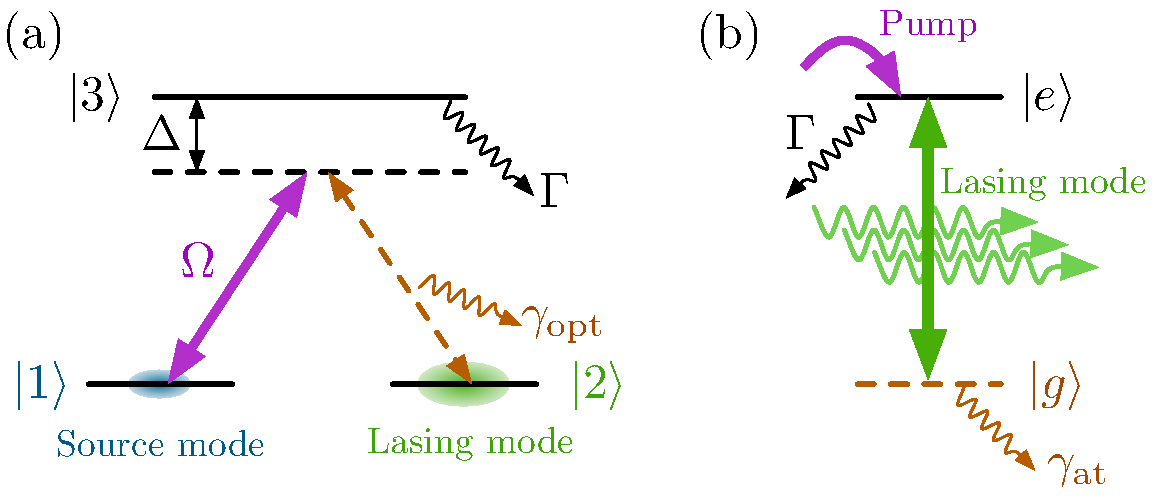
\includegraphics[width=14cm]{AtomLaserVsOpticalLaser}
    \caption{Comparison of the atom laser pumping scheme considered in this chapter (a) to the typical optical laser pumping scheme (b).  In an optical laser absorption of lasing mode photons by atoms in the state $\ket{g}$ is suppressed by the fast decay of these atoms to lower atomic levels (represented by a decay process with rate constant $\gamma$).  This fast decay is what makes the pumping process irreversible.  This irreversibility in the atom laser pumping mechanism derives from the departure of the photons emitted on the $\ket{2} \leftrightarrow \ket{3}$ transition.  Once a photon in this mode leaves the system the lasing mode atom cannot be transferred back to the source mode via the excited state $\ket{3}$.\label{OpticalPumping:AtomLaserVsOpticalLaser}}
\end{figure}

The optical pumping process under investigation in this chapter is illustrated in \figureref{OpticalPumping:AtomLaserVsOpticalLaser}(a).  In this process atoms in the source mode are driven by a laser into an excited state from which they can decay into the lasing mode (the condensate).  Although there is no laser driving this second transition ($\ket{3}\leftrightarrow\ket{2}$), the decay of atoms into the lasing mode is not spontaneous emission in the usual sense.  The emission process is \emph{atomically}-stimulated by the large occupation of the lasing mode in the same way that the transition may be \emph{optically}-stimulated even in the absence of any population in the atomic state into which the atom decays.

The final decay of an atom into the lasing mode in \figureref{OpticalPumping:AtomLaserVsOpticalLaser} resembles standard \emph{optical} laser schemes [see \figureref{OpticalPumping:AtomLaserVsOpticalLaser}(b)] in which the roles of atoms and light are reversed.  In an optical laser an atom in the excited state is stimulated to emit into the ground state by the resonant photons in the laser cavity.  Once the atom has emitted, it decays rapidly into other internal states with rate $\gamma$ significantly limiting reabsorption from the $\ket{g}$ state.  A similar process occurs in the proposed optical pumping scheme in which the photon emitted as the atom decays  leaves the system rapidly preventing reabsorption.  The loss of photons from the system is represented by the decay of the optical mode with rate $\gamma$ in \figureref{OpticalPumping:AtomLaserVsOpticalLaser}(a).

This similarity between the proposed atom laser pumping mechanism and the usual optical laser pumping mechanism is clearly illustrated by considering the Hamiltonian coupling the excited and ground atomic states in \figureref{OpticalPumping:AtomLaserVsOpticalLaser}
\begin{align}
    \hat{H} &= \hbar \epsilon \left(\hat{a}_e^\dagger \hat{a}_g \hat{a}_\text{ph} + \hat{a}_g^\dagger \hat{a}_\text{ph}^\dagger \hat{a}_e  \right),
    \label{OpticalPumping:TwoLevelAtomHamiltonian}
\end{align}
where $\epsilon$ is a real coupling constant, the $\hat{a}_e$, $\hat{a}_g$, and $\hat{a}_\text{ph}$ are annihilation operators for the atomic excited state, atomic ground state and photon mode respectively.  The rotating wave approximation has been made in obtaining this Hamiltonian, assuming that the optical mode is not detuned from the atomic transition by a large fraction of the frequency difference between the two states.  

The Hamiltonian \eqref{OpticalPumping:TwoLevelAtomHamiltonian} describes both the atom- and optical-laser pumping mechanisms, the difference in the mechanisms being in the occupations of the various states.  If the system is initially in a state with $N_e$ atoms in the atomic excited state, $N_g$ atoms in the atomic ground state and $N_\text{ph}$ photons in the optical mode, the amplitude for an atom in the excited state to emit a photon is
\begin{align}
    \bra{N_e-1, N_g + 1, N_\text{ph} + 1} \hat{H} \ket{N_e, N_g, N_\text{ph}} &= \hbar \epsilon \sqrt{N_g+1} \sqrt{N_\text{ph}+1} \sqrt{N_e}.
\end{align}
This emission process can therefore be stimulated either by photons ($N_\text{ph} > 0$) or by atoms ($N_\text{g} > 0$).  It would also be possible for the emission to be stimulated by both photons \emph{and} atoms, although in this case the amplitude for the absorption process would be non-zero
\begin{align}
    \bra{N_e+1, N_g - 1, N_\text{ph} - 1} \hat{H} \ket{N_e, N_g, N_\text{ph}} &= \hbar \epsilon \sqrt{N_e+1} \sqrt{N_\text{ph}} \sqrt{N_g}.
\end{align}
It is for this reason that it is desirable in an optical laser to have $N_g \approx 0$, and in the proposed atom laser pumping scheme to have $N_\text{ph} \approx 0$.

Atom laser pumping schemes of the form of that illustrated in \figureref{OpticalPumping:AtomLaserVsOpticalLaser}(a) have been proposed before~\citep{Olshanii:1996,Janicke:1996,Spreeuw:1995,Cirac:1996rr,Cirac:1996,Santos:2000,Castin:1998,Cirac:1994,Vengalattore:2003,Santos:2001ve,Wolf:2000,Santos:1999qf} for the production of BEC without the use of collisional evaporation and its consequent losses.  The main problem that they all seek to address is that of reabsorption of photons spontaneously emitted when the atom in state $\ket{3}$ decays to the $\ket{2}$ state, but not to the lasing mode.  This emitted photon will be resonant with the lasing mode and may be scattered several times before finally leaving the condensate.  A single such spontaneously emitted photon can cause significant heating of a condensate as the single photon recoil energy can be as large as or greater than the chemical potential of the condensate.

One proposed method~\citep{Castin:1998,Vengalattore:2003} for reducing the heating uses a purely geometric solution: if a condensate is made sufficiently narrow in one or more dimensions such that a photon emitted in one of those directions is negligibly likely to be reabsorbed, the overall probability for reabsorption will also be reduced.  While this method may be appropriate for the initial formation of BEC, it is impractical for a large BEC as the trap deformation necessary to reach the required regime is extreme.  For a \nucl{87}{}{Rb} condensate of $N= 5\times 10^5$ atoms with trapping frequencies of $\omega_x = \omega_y = \unit[2\pi \times 128]{Hz}$, $\omega_z = \unit[12.8]{Hz}$, the mean-free path in the centre of the condensate for a resonant photon on the cycling transition ($\lambda = \unit[780]{nm}$) is $1/(n \sigma) = \unit[16]{nm}$ where $n$ is the peak condensate density and $\sigma = 3 \lambda^2/2 \pi$ is the atomic scattering cross-section.

Another possibility for reducing reabsorption that works well in optical lattices is to operate in the \emph{festina lente} regime~\citep{Wolf:2000,Santos:1999qf,Cirac:1996,Castin:1998} in which the energy levels of the trap are sufficiently separated such that a photon emitted when an atom decays into a particular trap level is only resonant with atoms in that level (and those levels degenerate with it).  This prevents the occurrence of `dangerous' processes in which an excited atom decays into a non-condensate level with the emitted photon being absorbed by the condensate.  In the case of resonant optical pumping light ($\Delta = 0$ in \figureref{OpticalPumping:AtomLaserVsOpticalLaser}(a)), the \emph{festina lente} regime requires that $\omega_\text{min} \gg \Gamma$  where $\omega_\text{min}$ is the minimum of the magnetic trapping frequencies.  Strictly, the \emph{festina lente} regime has only been investigated in the absence of \emph{s}-wave scattering interactions, however one would expect that in the presence of \emph{s}-wave scattering the trap frequency energy scale would simply be replaced by the energy of the relevant Bogoliubov excitation (refer to \sectionref{Peaks:ElementaryExcitations}).  Regardless, the \emph{festina lente} regime is impractical to achieve in alkali gases like \nucl{87}{}{Rb} as the relevant decay rate is $\Gamma = \unit[2\pi\times 5.9]{MHz}$, which is much larger than typical trap frequencies ($\omega \sim \unit[2\pi \times 100]{Hz}$) and condensate excitations ($\mu/\hbar \sim \unit[2\pi \times 10]{kHz}$).

A third possibility for reducing reabsorption is to operate in the \emph{boson accumulation regime} (BAR)~\citep{Cirac:1996rr,Floegel:2001} in which an atom in the excited state is significantly more likely to decay into the condensate mode than into all other modes.  In this limit it can be shown that absorption of emitted photons by atoms not in the condensate mode can be neglected.  It is in the BAR that we wish to operate our proposed pumping mechanism of \figureref{OpticalPumping:AtomLaserVsOpticalLaser}(a).  

Up to this point, the source mode was entirely arbitrary; without consideration of reabsorption the proposed pumping process would work equally well for coherent or thermal states in the source mode.  As the optical transition between the excited atomic state and the lasing mode is not driven by a laser, the phase of the photons emitted is determined by the relative phase between the source and lasing modes; the direction of population transfer does not depend on the phase difference between these two modes. However the requirement that excited atoms be significantly more likely to decay into the condensate mode than to any other mode places a stringent requirement on the source mode of the pumping mechanism.  For this requirement to be satisfied, the momentum width of the source atom distribution cannot be significantly larger than the momentum width of the condensate.  If this were not the case a significant fraction of the atoms would not be momentum-resonant with the condensate under the pumping process and will therefore not be in the boson accumulation regime.  These atoms would be able to reabsorb spontaneously emitted photons causing the reabsorption problem previously discussed.  For an atomic distribution to have a momentum width comparable to that of the target condensate, the atoms must either be condensed or if they are thermal, be trapped in a significantly weaker trap than the target condensate mode and have a temperature below the condensation temperature in the tighter trap.  

Although it would be desirable to be able to use a thermal source of atoms as the source mode, the remainder of this chapter will investigate the possibility of using a coherent source of atoms as the source mode of the pumping mechanism.  Specifically, this coherent source will be an atom laser extracted from a second, source condensate.  Continuous operation of this scheme could in principle be achieved by replacing the source condensate with an independently-produced condensate once it is depleted.  As the pumping mechanism is independent of the phase-difference between the source and lasing modes this will not affect the direction of population transfer.

% \parasep
% 
% The pumping mechanism described in this section bears some resemblance to other optical processes that can occur in Bose-Einstein condensates such as EIT, and Rayleigh/Raman superradiance. FIXME: Complete paragraph/s.
% 
% Quote from the paper:
% 
% The mechanism we have described for pumping is related to pulsed Raman super-radiance that has been studied previously.  In our work, in the laboratory frame, atoms are driven from the $\ket{2, 0}$ untrapped state into the $\ket{1, -1}$ trapped state enabling us to continue pumping indefinitely.  the condensate that we pump is stationary in the laboratory frame.  Furthermore, our experiment is carried out in a double-condensate geometry with internal states that enable simultaneous pumping and outcoupling to produce a freely propagating atom laser beam from a simultaneously pumped condensate.
% 
% There is a second mechanism that we have considered that is related to the EIT mechanism described in the work by~\citet{Ginsberg:2007fk}.  Similar to the existing Raman super-radiance experiments, their work was necessarily carried out in a pulsed regime.  In our experiment, again, the geometry and choice of internal states enable the possibility of carrying out a related experiment continuously.  The condensates in such an experiment must have some spatial overlap.  The $\ket{2, 0}$ atoms are produced in the overlap region where the $\pi$-polarised pump beam is absorbed and the $\sigma$-polarised beam is produced.  Both beams travel in the same direction.  The amplitude of the $\pi$-polarised beam decays in the overlap region.  The amplitude of the $\sigma$-polarised beam grows.  The atoms follow the dark state and are pumped continuously to the lasing mode.


\section{The continuous pumping experiment}
\label{OpticalPumping:ContinuousExperiment}

A summary is provided here of the continuous pumping experiment performed by \emph{Nick Robins}, \emph{Cristina Figl} and \emph{Matthew Jeppesen} at the Department of Quantum Science, ANU.  Further details of the experimental setup and results are published in \citet{Robins:2008}.

\begin{figure}
    \centering
    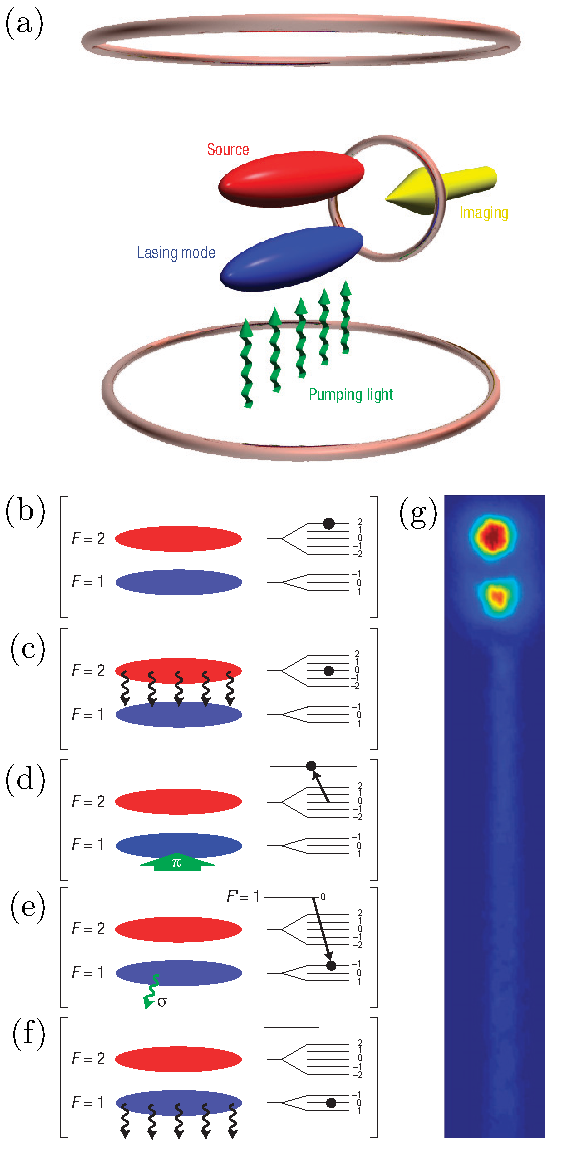
\includegraphics[width=8cm]{ExperimentSchematic}
    \caption{Schematic diagram of the experiment (a) and pumping steps (b--f).  A radiofrequency field spin-flips the atoms to the $\ket{2, 0}$ state (b), and they fall under gravity (c).  The light field couples the atoms to the $F'=1$ excited state from which they are stimulated to emit into the $\ket{1, -1}$ BEC.  The atomic momentum is cancelled by the absorption and emission of the photons (d, e).  A second radiofrequency field finally output-couples the atoms into the $\ket{1, 0}$ atom laser (f).  (g), Absorption image of the experimental system, showing source, laser mode and output beam.}
    \label{OpticalPumping:ExperimentSchematic}
\end{figure}

\begin{table}
    \centering
    \begin{tabular}{cc}
    \toprule
    Parameter & Value\\
    \midrule
    $\ket{F=2, m_F=2}$ (source) condensate number & $N_\text{source} = (6.7 \pm 0.5)\times 10^5$ \\
    $\ket{F=1, m_F=-1}$ (laser) condensate number & $N_\text{laser} = (5.0 \pm 0.4) \times 10^5$ \\
    Radial trapping frequency (for $\ket{1, -1}$) & $\omega_r = \unit[2\pi \times 130]{Hz}$ \\
    Axial trapping frequency (for $\ket{1, -1}$) & $\omega_z = \unit[2\pi \times 13]{Hz}$ \\
    \bottomrule
    \end{tabular}
    \caption{Experimental parameters for the Rubidium-87 BEC system under consideration.}
    \label{OpticalPumping:ExperimentalParameters}
\end{table}


To produce a pumped atom laser two independent condensates are prepared in the $\ket{F=2, m_F=2}$ and $\ket{F=1, m_F=-1}$ magnetically trapped states of \nucl{87}{}{Rb}.  Owing to their larger magnetic moment, the $\ket{2, 2}$ atoms are more tightly confined in the magnetic field than the $\ket{1, -1}$ atoms, and hence the evaporation does not directly cool them.  They are, however, sympathetically cooled through elastic collisions with the $\ket{1, -1}$ atoms~\citep{Myatt:1997}.  For the condensate numbers and trapping frequencies given in \tableref{OpticalPumping:ExperimentalParameters} the Thomas-Fermi radius of each cloud is approximately $\unit[5]{\micro m}$ in the vertical direction.  The different magnetic moments of the two clouds lead to a gravitational sag between their centres of $\unit[8]{\micro m}$. Hence, the two clouds of atoms overlap only slightly, with the $\ket{2, 2}$ source condensate located above the $\ket{1, -1}$ laser-mode condensate [see \figureref{OpticalPumping:ExperimentSchematic}(a)].

To measure the effect of pumping, it is essential that the number of atoms in each state is stable from one experimental run to the next.  For this purpose, many details of the apparatus were refined, including very efficient baffling against stray resonant light, very low uncertainty and drift in laser frequency, intensity and polarisation, and good vibrational and thermal stability of the trap.  The stability of the number of atoms in each state was determined for a data set comprising 20 measurements, and found to be as low as 1\%.

The operation of the experiment is illustrated in \figureref{OpticalPumping:ExperimentSchematic}.  Starting with an initial number of atoms in each state [\figureref{OpticalPumping:ExperimentSchematic}(b)], a weak continuous radiofrequency field is applied to the upper source cloud which couples atoms from the $\ket{2, 2}$ state, through $\ket{2, 1}$ to the $\ket{2, 0}$ state.  This coupling is highly spatially selective and does not affect the $\ket{1, -1}$ cloud.  These atoms begin to fall away from the $\ket{2, 2}$ source cloud [\figureref{OpticalPumping:ExperimentSchematic}(c)].  Simultaneously approximately $\unit[10]{pW}$ of upward propagating $\pi$-polarised light resonant with the $\ket{F=2}\rightarrow\ket{F'=1}$ transition is applied.  Although this light is resonant in energy with the $\ket{2, 2}$ source atoms, they are prevented from absorbing photons by atomic selection rules.  Hence, the source cloud is unaffected by the pumping light.  For pumping the laser mode, the $\ket{2, 0}$ atoms will absorb the pumping light [\figureref{OpticalPumping:ExperimentSchematic}(d)].  As these atoms fall, they may make a transition into the excited $\ket{F'=1, m_F=0}$ state from which they are stimulated to emit into the laser mode $\ket{1, -1}$ by the atoms already present in that mode [\figureref{OpticalPumping:ExperimentSchematic}(e)].  The $\sigma^{+}$-photon emitted in this process carries the phase difference between the pump atoms and the condensate.  Finally, the $\ket{1, -1}$ laser-mode atoms are output-coupled to produce the atom laser beam in the $\ket{1, 0}$ state [\figureref{OpticalPumping:ExperimentSchematic}(f)].  An absorption image of the ultracold atoms used to build the pumped atom laser system is shown in \figureref{OpticalPumping:ExperimentSchematic}(g).

For successful pumping, the pump atoms must be momentum-resonant with the lasing condensate.  This means that their atomic velocity after the emission of the photon has to lie within the velocity spread of the BEC.  The magnetic trapping frequencies were chosen not only to position the two clouds as closely as possible without significant overlap, but also such that the velocity acquired by a $\ket{2, 0}$ atom in falling from the centre of the $\ket{2, 2}$ cloud to the centre of the $\ket{1, -1}$ laser mode ($\unit[12]{mm\, s\textsuperscript{-1}}$) can be cancelled by the absorption of an appropriately directed and phased $\sigma^{+}$-photon; a single-photon recoil corresponds to $\unit[6]{mm\, s\textsuperscript{-1}}$.  The velocity at the laser-mode centre can be tuned by around $\unit[\pm 2]{mm\, s\textsuperscript{-1}}$ by moving the coupling surface within the source cloud up or down.  While the pump atoms are falling through the $\ket{1, -1}$ laser mode, the velocity varies by $\unit[\pm 3]{mm\, s\textsuperscript{-1}}$ owing to gravity and the time for which the pumping atoms satisfy momentum resonance with the laser mode is much shorter ($\sim \unit[100]{\micro s}$) than the traversal time across the laser mode ($\sim\unit[1]{ms}$).  The velocity spread of the laser mode is of the order of $\unit[0.3]{mm\, s\textsuperscript{-1}}$; thus, cancelling the atomic momentum of the $\ket{2, 0}$ state requires an extreme level of control over pumping parameters.  In the experiment no collective motion, such as sloshing or breathing of either the source- or laser-mode condensates was observed.  This implies that if excitations driven by the pumping exist, they occur with an amplitude of less than 5\% of the full-width at half-maximum of the laser-mode condensate, which was inferred from the resolution limit of the imaging system.

\begin{figure}
    \centering
    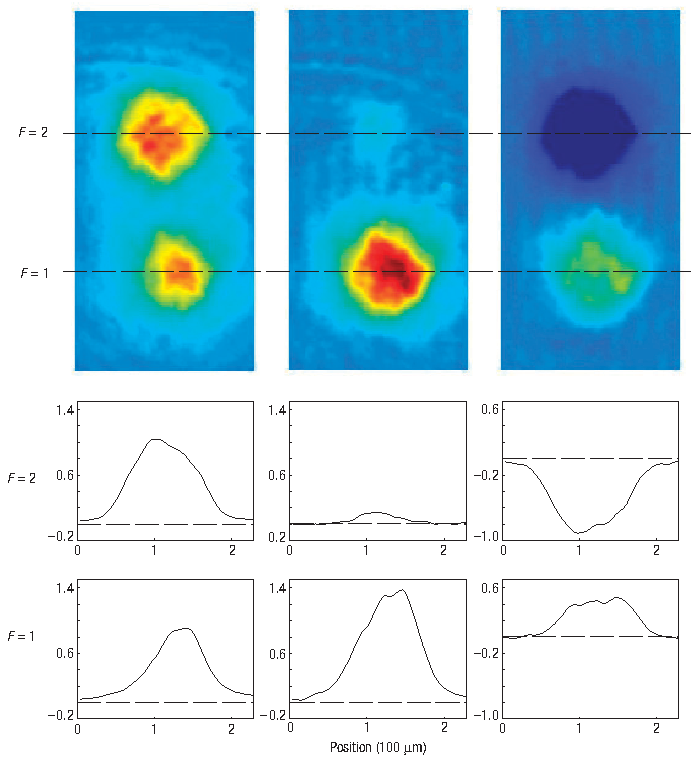
\includegraphics[width=12cm]{ExperimentalResults}
    \caption{Blue-detuned absorption images averaged over three identical runs of the experiment (top row); detuning of the imaging laser from resonance is $\unit[7]{MHz}$.  The graphs below are horizontal cross-sections through the absorption images, showing optical depth, averaged over $\unit[50]{\micro m}$ in the vertical direction.  The three columns correspond to: pumping off (left); pumping on (centre); difference between pumped and unpumped (right).}
    \label{OpticalPumping:ExperimentalResults}
\end{figure}

To isolate and study the pumping mechanism, the experiment was first operated without outcoupling from the laser-mode condensate.  \figureref{OpticalPumping:ExperimentalResults} demonstrates the effect \unit[200]{ms} of pumping has on the $\ket{1, -1}$ condensate; the left-hand image is taken without outcoupling from either condensate and without the pumping light.  The absorption image shows the unpumped $F=1$ laser-mode BEC (the lower cloud) with the $F=2$ source atoms above.  The curves below are horizontal cross-sections through the absorption images showing the optical depth of each atom cloud.  The central image shows the effect of \unit[200]{ms} of pumping on the laser-mode BEC.   The source is almost completely depleted and the laser-mode atom number has increased to $(7.2 \pm 0.4)\times 10^5$.  The third column shows the difference between the pumped and unpumped images. It is important to note that the profile of the laser-mode condensate after pumping has a significant Thomas-Fermi component with a small increase in the Gaussian thermal component.  The pumping efficiency, which is defined as the growth of the laser mode compared with the loss from the source, is $(35 \pm 10)\%$ for the results presented in \figureref{OpticalPumping:ExperimentalResults}.

A second experiment was also performed simultaneously pumping the laser-mode BEC and outcoupling from this condensate to demonstrate that the production of the atom laser could be operated independently of the pumping mechanism into the condensate.  In this chapter we focus on the results of the first experiment in which the pumping mechanism was studied.

\parasep

The continuous pumping experiment just described was designed to transfer $2 \hbar k$ of momentum to the falling $\ket{2, 0}$ atoms (by absorbing a photon of momentum $\hbar k$ going up and then emitting a photon of similar momentum directed downwards) as they are transferred to the laser-mode condensate.  However, there is a second way for these atoms to be momentum-resonant with the laser-mode condensate.  If the outcoupling surface for the upper condensate is towards the lower edge of the condensate the outcoupled atoms will be in close proximity to the laser-mode condensate immediately below due to the slight spatial overlap.  These recently outcoupled atoms will have almost no momentum and will be able to absorb a $\pi$-polarised photon with momentum $\hbar k$ upwards and emit a $\sigma^+$-polarised photon of similar momentum also directed upwards, decaying into the lower laser-mode condensate with no net momentum transfer.  These two processes are illustrated in \figureref{OpticalPumping:WhichWayDidThePhotonsGo?}.

Which process is occurring has a significant impact on the potential to extend this experimental scheme to the operation of a continuously pumped atom laser.  It was envisaged that this experiment could be extended to the production of a continuously pumped atom laser by replacing the source condensate once it becomes depleted with an independently produced condensate.  If it is the $0 \hbar k$ momentum-transfer process that is occurring, the source and lasing condensates must have a slight spatial overlap for the pumping mechanism to operate.  The source condensate will therefore not be able to be replaced once depleted without disturbing the lasing condensate.  If it is the $2 \hbar k$ momentum-transfer process that is occurring, the source and lasing condensates can be spatially separated, and in principle the source condensate could be replaced without any disruption to the lasing condensate.  Determining which of the two processes operated in the pumping experiment is therefore crucial to determining the viability of a continuously pumped atom laser based on this scheme.

These two different processes are examined in greater detail theoretically in \sectionref{OpticalPumping:MultimodeModel}, however we begin our theoretical analysis of the experiment and the pumping mechanism more generally with a simple single-mode model of the process illustrated in \figureref{OpticalPumping:AtomLaserVsOpticalLaser}(a).

\begin{figure}
    \centering
    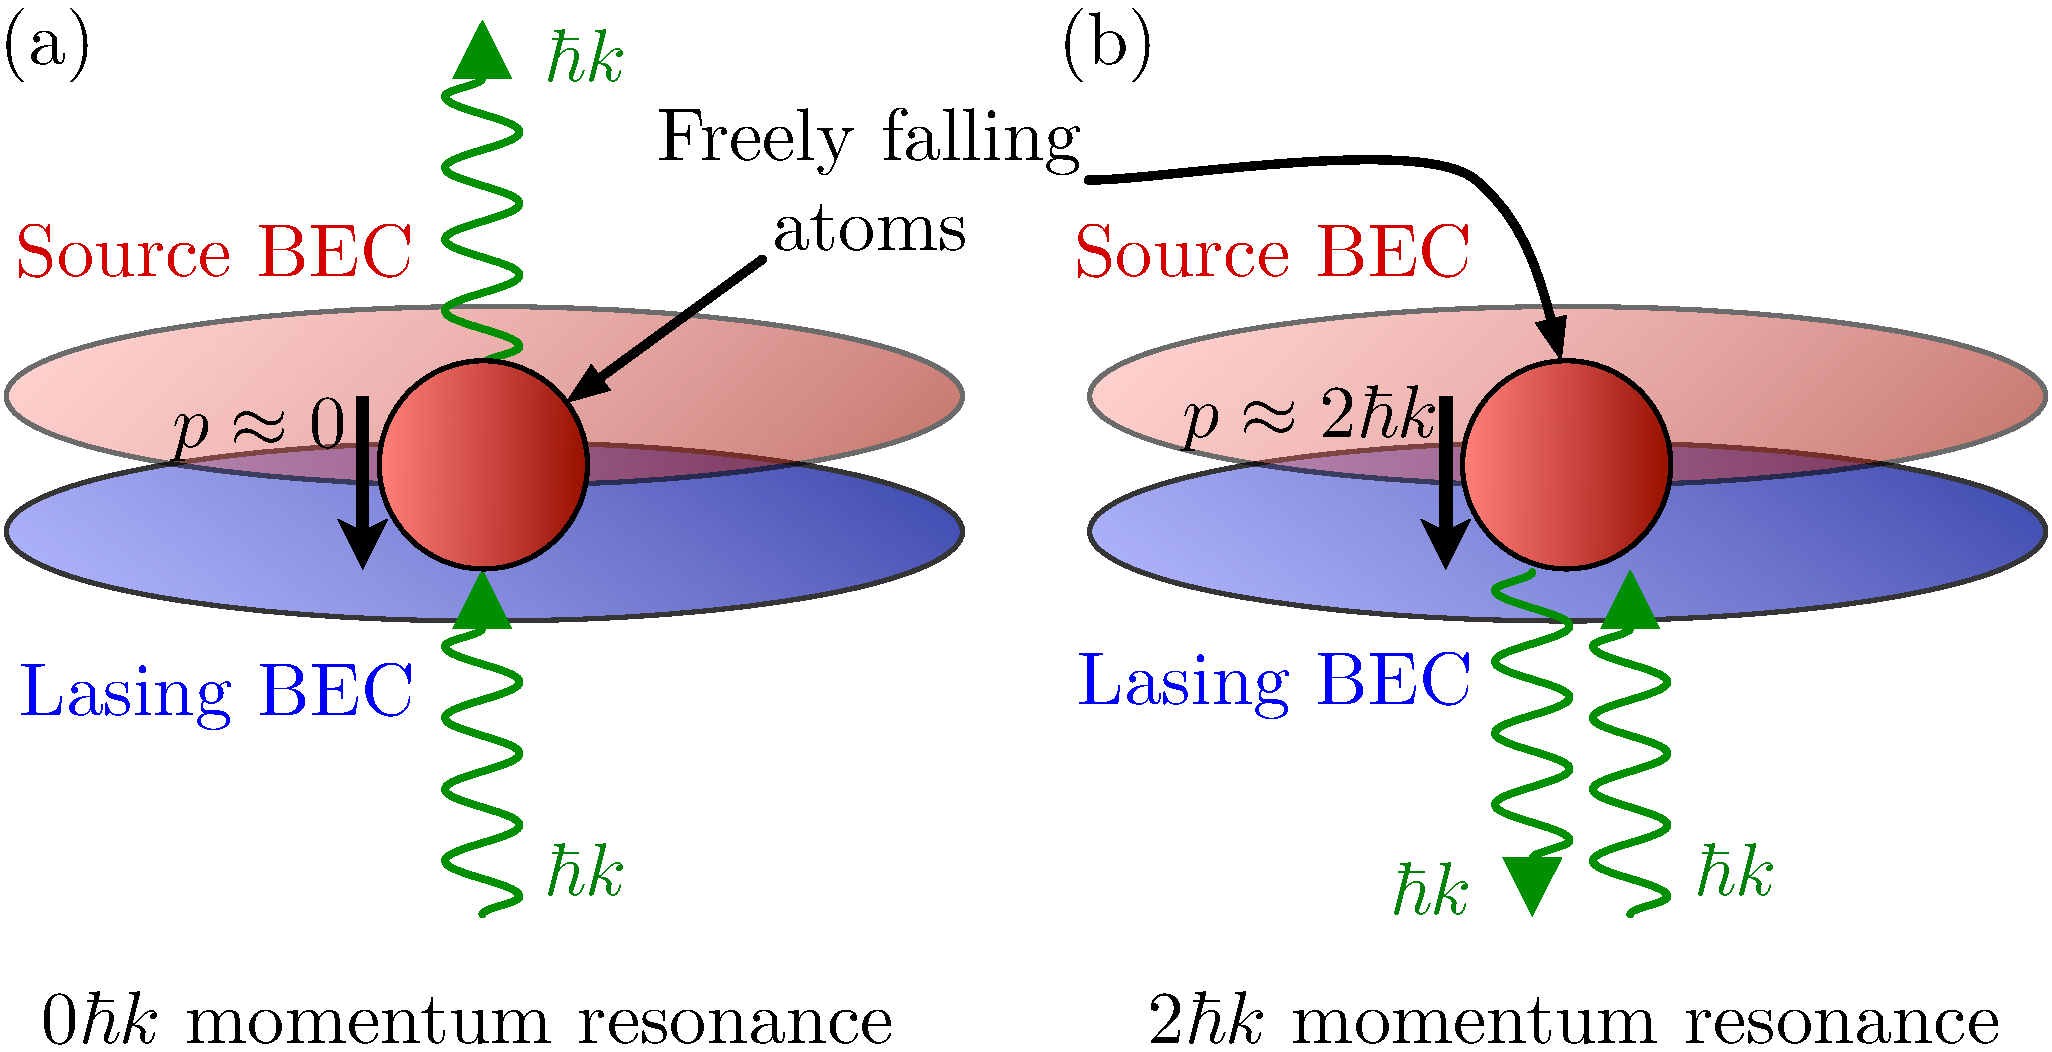
\includegraphics[width=12cm]{WhichWayDidThePhotonsGo?}
    \caption{Illustration of the two potential pumping processes that could occur in the continuous pumping experiment.  The freely-falling atoms form the atom laser in the $\ket{2, 0}$ state and can undergo stimulated transitions into the lasing condensate in one of two processes.  If the atoms are outcoupled from the lower part of the source condensate, they may immediately absorb a pumping photon from below and emit one in the same direction to decay into the lasing condensate with no net change in momentum (a).  If the atoms are outcoupled from the centre of the source condensate, they may fall under gravity for approximately $\unit[1]{ms}$ gaining approximately $2 \hbar k$ of momentum before absorbing a pumping photon from below and emitting one downwards to decay into the source condensate with a net momentum transfer of $2 \hbar k$ (b).}
    \label{OpticalPumping:WhichWayDidThePhotonsGo?}
\end{figure}


\section{Simple single-mode model}
\label{OpticalPumping:SingleModeModel}

We begin our theoretical investigation of the pumping mechanism behind the previously-described experiment by considering the simplest-possible model, a single-mode mean-field approximation to the process illustrated in \figureref{OpticalPumping:AtomLaserVsOpticalLaser}(a).  The equations of motion for this model are
\begin{subequations}
    \label{OpticalPumping:SingleModeModel}
    \begin{align}
        \frac{d}{dt} c_\text{source} &= -i \Omega^* c_\text{excited} \\
        \frac{d }{dt}c_\text{excited} &= -i \Omega c_\text{source} -i g \alpha c_\text{lasing} - i \Delta c_\text{excited} - \frac{\Gamma}{2} c_\text{excited}\\
        \frac{d }{dt}c_\text{lasing} &= -i g^* \alpha^* c_\text{excited} \\
        \frac{d }{dt}\alpha &= -i g^* c_\text{lasing}^* c_\text{excited}^{\phantom{*}} - \frac{\gamma}{2} \alpha,
    \end{align} 
\end{subequations}
where $c_\text{source}$, $c_\text{lasing}$ and $c_\text{excited}$ are the amplitudes of the source $\ket{1}$, lasing $\ket{2}$ and excited $\ket{3}$ modes respectively, $\Omega$ is the complex Rabi frequency due to the pumping laser coupling the source and excited modes with detuning $\Delta$, $\alpha$ is the amplitude of the optical mode into which the excited atoms emit when decaying into the lasing mode and $g$ is the complex coupling constant for this transition.  The optical mode $\alpha$ will decay as photons propagate away from the system.  This process is modelled phenomenologically with a loss rate $\gamma$ from the optical mode $\alpha$.  The spontaneous decay of the excited state into modes other than the lasing mode occurs at a rate $\Gamma$.  It has been assumed that the pumping laser is sufficiently strong to be negligibly absorbed.  This assumption is relaxed in \sectionref{OpticalPumping:MultimodeModel}.  The evolution equations \eqref{OpticalPumping:SingleModeModel} are given in a rotating frame in which the energy difference between the source, excited and lasing modes have been appropriately removed.

In deriving \eqref{OpticalPumping:SingleModeModel} it has been assumed that atoms that undergo spontaneous decay from the excited mode will have no further impact upon the system.  In particular this means that the absorption of photons in the $\alpha$ mode by atoms in modes other than the lasing mode has been neglected.  The absorption of these photons by the lasing mode is, however, retained.  As discussed in \sectionref{OpticalPumping:PumpingMechanism} this is a valid approximation in the boson accumulation regime in which an excited atom is significantly more likely to decay into lasing mode than into any other mode.

The long-term dynamics of \eqref{OpticalPumping:SingleModeModel} will determine the usefulness of the process as a pumping mechanism.  The fast-timescale behaviour of this system can therefore be eliminated.  By far the fastest process in the system is the decay of the photons in the $\alpha$ mode as they leave the system.  The time taken for a photon to cross the width of a typical condensate ($\sim\unit[10]{\micro m}$) is $\sim\unit[10^{-13}]{s}$, giving $\gamma \sim \unit[10^{13}]{s\textsuperscript{-1}}$.  By comparison, the spontaneous decay rate of the excited mode is $\Gamma \sim \unit[10^8]{s\textsuperscript{-1}}$ for the $F'=1$ manifold of \nucl{87}{}{Rb}.  As the $\alpha$ mode reaches a quasistationary value on the fastest timescale in the system ($\gamma$), it can be adiabatically eliminated and replaced with its quasistationary limit,
\begin{align}
    \alpha & \approx -\frac{2 i g^*}{\gamma} c_\text{lasing}^* c_\text{excited}. \label{OpticalPumping:Alpha}
\end{align}

We next assume that the pump laser is driving the atoms in the weak-field regime, $\Omega \ll \max\left(\Delta, \Gamma\right)$.  In this limit, the excited mode $c_\text{excited}$ evolves on a more rapid timescale than either the source or lasing modes.  The excited mode may therefore also be adiabatically eliminated and replaced with its long-term average
\begin{align}
    c_\text{excited} &\approx \frac{-i \Omega c_\text{source}}{\frac{1}{2}\Gamma + 2 \frac{\abs{g}^2}{\gamma} N_\text{lasing} + i \Delta}, \label{OpticalPumping:CExcited}
\end{align}
where $N_\text{lasing} = \abs{c_\text{lasing}}^2$ is the number of atoms in the lasing mode.

With these two adiabatic eliminations made, the rate equations for the populations of the remaining two modes are obtained by substituting \eqref{OpticalPumping:Alpha} and \eqref{OpticalPumping:CExcited} into \eqref{OpticalPumping:SingleModeModel},
\begin{subequations}
    \label{OpticalPumping:SingleModeRateEquations}
    \begin{align}
        \frac{d}{dt} N_\text{source} &= - \frac{\abs{\Omega}^2 \left(\Gamma + \Gamma'\right)}{\abs{\frac{1}{2}(\Gamma + \Gamma') + i \Delta}^2} N_\text{source}\\
        \frac{d}{dt} N_\text{lasing} &= \frac{\Gamma'}{\Gamma + \Gamma'} \left( - \frac{d}{dt} N_\text{source}\right),
    \end{align}
\end{subequations}
where $\displaystyle \Gamma' = 4 \frac{\abs{g}^2}{\gamma} N_\text{lasing}$ is the rate constant with which atoms in the excited mode decay into the lasing mode.

The efficiency of the transfer of atoms in the pumping process is $\Gamma'/(\Gamma + \Gamma')$, which behaves as expected: as the occupation of the lasing mode $N_\text{lasing}$ is increased, the efficiency increases due to bosonic stimulation.  What is perhaps not expected is the behaviour of the transfer rate constant.  In the limit of large detuning, $\Delta \gg \Gamma + \Gamma'$, the rate constant for atom transfer is
\begin{align}
    \left.-\frac{d}{dt} N_\text{source}\middle/N_\text{source}\right. &\approx \frac{\abs{\Omega}^2}{\Delta^2} \left(\Gamma + \Gamma'\right), \label{OpticalPumping:SingleModePumpingRateLargeDetuning}
\end{align}
which increases as the lasing mode population increases (due to increasing $\Gamma'$).  In the limit of small detuning however ($\Delta \ll \Gamma + \Gamma'$) very different behaviour is obtained
\begin{align}
    \left.-\frac{d}{dt} N_\text{source}\middle/N_\text{source}\right. &\approx 4 \frac{\abs{\Omega}^2}{\Gamma + \Gamma'}, \label{OpticalPumping:SingleModePumpingRateZeroDetuning}
\end{align}
which \emph{decreases} as the lasing mode population increases.  This behaviour is due to the depletion of the excited state as $\Gamma'$ increases.  In the limit of small detuning, spontaneous and stimulated decay are the fastest processes reducing the occupation of the excited state, hence increasing those rates will reduce the overall population of the excited state.  In this limit as the excited state population decreases proportional to the squared sum of these rates
\begin{align}
    N_\text{excited} &\approx 4 \frac{\abs{\Omega}^2}{(\Gamma + \Gamma')^2} N_\text{source},
\end{align}
the overall rate of atom transfer is suppressed as these processes occur on faster timescales.  In the opposite limit of large detuning, the spontaneous and stimulated decay processes are a perturbation on the Rabi-flopping process which populates the excited state.  In this limit the excited state population is independent of the spontaneous and stimulated emission rates
\begin{align}
    N_\text{excited} &\approx \frac{\abs{\Omega}^2}{\Delta^2} N_\text{source},
\end{align}
and the overall atom transfer rate into the lasing mode can be Bose-enhanced.

\parasep

The simple model developed in this section can be applied to the continuous pumping experiment described in \sectionref{OpticalPumping:ContinuousExperiment} to give a limit for the efficiency of the `$2 \hbar k$' momentum-transfer process.  In this process falling atoms outcoupled from the upper condensate reach a momentum of $2\hbar k$ vertically downwards before absorbing a pump photon of momentum $\hbar k$ from below and emitting a photon of similar momentum directed downwards to decay into the lasing mode.  If it is assumed that the intensity of the pump mode is approximately constant throughout the system, then the rate of transfer of atoms into the lasing mode cannot be faster than the rate of spontaneous emission while the source atoms are not momentum-resonant with the lasing mode\footnote{When the source atoms are not momentum-resonant with the lasing mode, it is equivalent to there being no atoms in the lasing mode.  In this case, $\Gamma'=0$ and from \eqref{OpticalPumping:SingleModePumpingRateZeroDetuning} it can be seen that the spontaneous emission rate must be greater than the transfer rate into the condensate.}.  An upper bound for the efficiency of the `$2 \hbar k$' momentum-transfer process should therefore be given by the ratio of the time for which the source atoms are momentum-resonant with the condensate ($\sim\unit[100]{\micro s}$, see \sectionref{OpticalPumping:ContinuousExperiment}) to the fall time for the atoms to that point ($\sim\unit[1]{ms}$).  As the upper bound for this process $(\sim 10\%)$ is lower than the observed efficiency $(\sim 35\%)$, either the transfer of atoms into the lasing mode must significantly reduce the intensity of the pump mode, or it must be the `$0 \hbar k$' process that operates in the continuous pumping experiment.  The argument used to obtain an upper bound for the efficiency of the `$2 \hbar k$' momentum-transfer process does not apply to the `$0 \hbar k$' momentum-transfer process in which atoms outcoupled from the upper condensate can be immediately pumped into the lower condensate.

The simple model considered in this section does not take into account the behaviour of the emitted photons in the $\alpha$ mode as they traverse the source and/or lasing modes as they leave the system.  The investigation of this and other multimode effects is the subject of the next section and will be shown to lead to modifications of the behaviour described by the simple single-mode model.

\section{Multimode model}
\label{OpticalPumping:MultimodeModel}

The multimode model we use in this chapter to describe the interaction of the BEC with the pumping light is similar to the Maxwell-Schrödinger equations \citep{Zobay:2005,Zobay:2006} used to describe superradiant Rayleigh scattering in BEC.  The difference here is that the pumping light may be much closer to resonance with the source atoms, and atoms can be stimulated to decay into a different internal atomic state from which they were excited (see the level diagram of \figureref{OpticalPumping:LevelDiagram}).

\begin{figure}
    \centering
    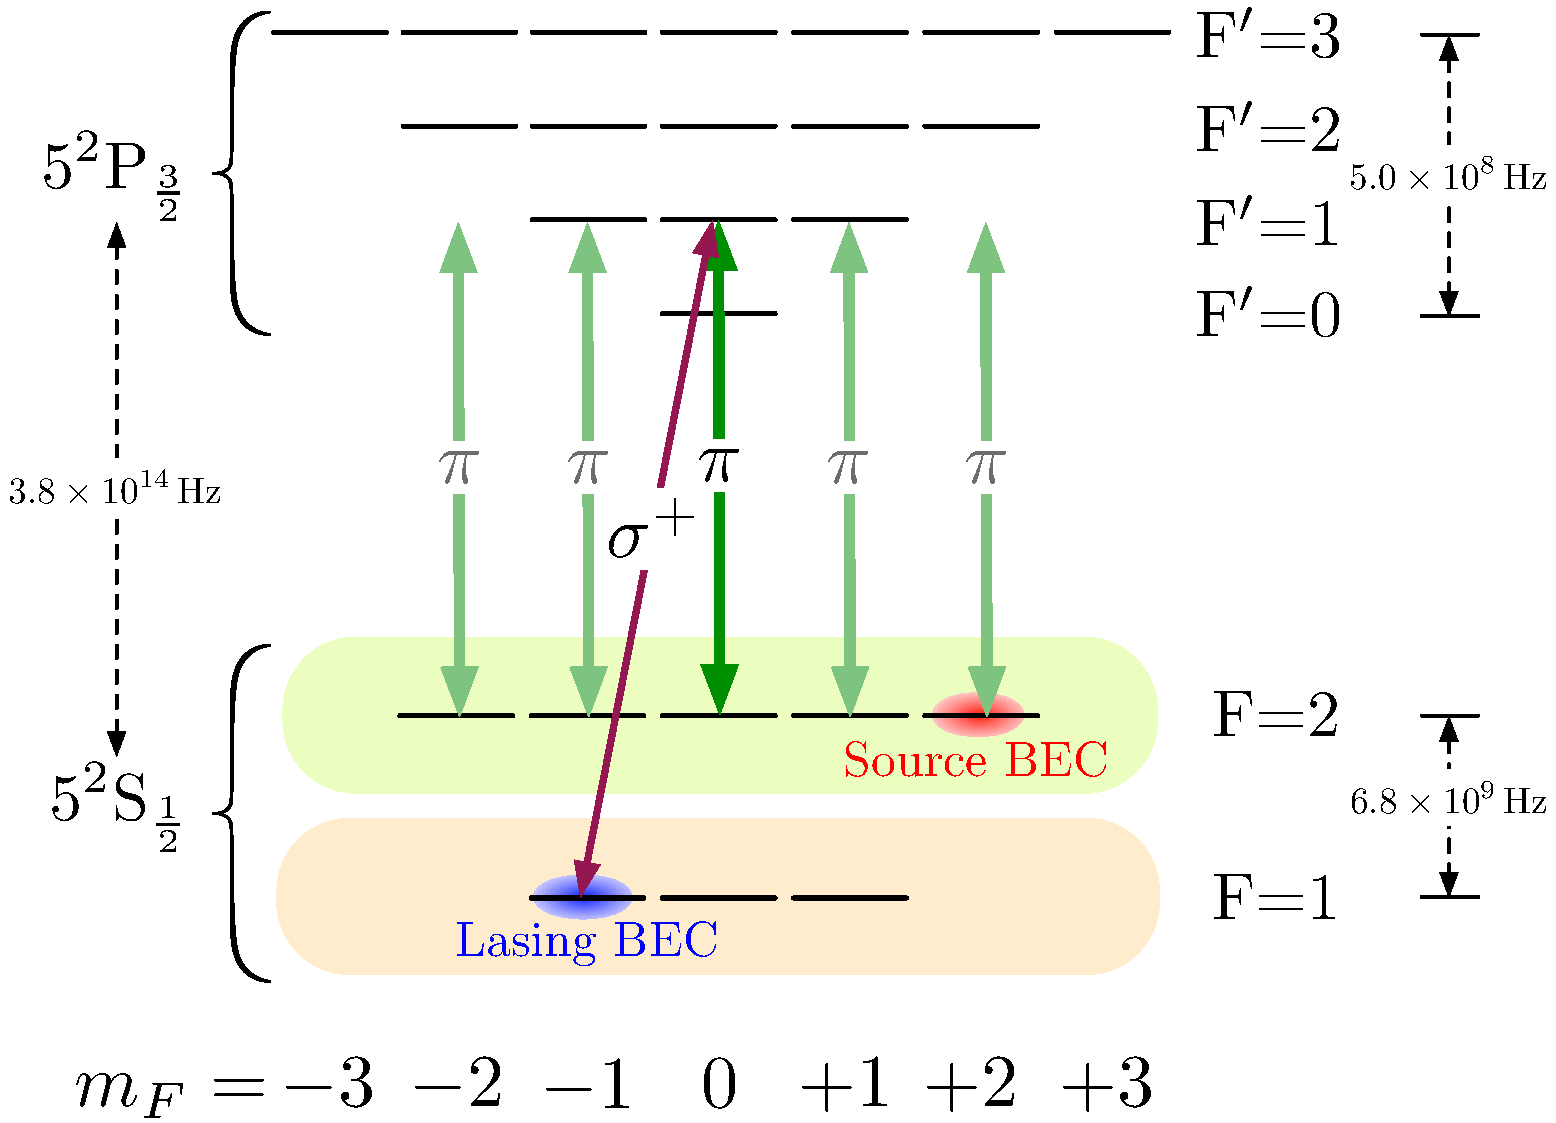
\includegraphics[width=13cm]{LevelDiagram}
    \caption{Level diagram for the continuous pumping experiment.  The $F=2 \leftrightarrow F'=1$ transitions are resonantly driven by $\pi$-polarised optical pumping light.  Although this light couples to several levels, its purpose is to drive $\ket{F=2, m_F=0}$ atoms into the $\ket{F'=1, m_F=0}$ state from which they may be stimulated to decay into the lasing BEC in the $\ket{F=1, m_F=-1}$ state and emit $\sigma^+$-polarised light.}
    \label{OpticalPumping:LevelDiagram}
\end{figure}

Although our aim is to model the continuous pumping experiment described in \sectionref{OpticalPumping:ContinuousExperiment}, we also wish to be able to consider the limit in which the pumping light is significantly detuned (by several GHz).  In either case, the only relevant optical transitions are those in the $\text{D}_2$ line (those pictured in \figureref{OpticalPumping:LevelDiagram}) as all other levels are sufficiently detuned to be negligibly populated.  The transitions closest in frequency to the $\text{D}_2$ line are those of the $\text{D}_1$ line which are detuned by $7 \times \unit[10^{12}]{Hz}$, significantly greater than the maximum expected detuning from the $\text{D}_2$ line.


\subsection{Model derivation}
\label{OpticalPumping:MultimodeModelDerivation}

We begin with the Hamiltonian for the combined atom--light system,
\begin{subequations}
    \label{OpticalPumping:AtomLightHamiltonian}
    \begin{align}
        \hat{H} &= \hat{H}_\text{atoms} + \hat{H}_\text{light} + \hat{H}_\text{atoms--light}, \\
        \begin{split}
            \hat{H}_\text{atoms} &= \sum_i \int d \vect{x}\, \hat{\Psi}_i^\dagger(\vect{x}) \left[ - \frac{\hbar^2 \nabla^2}{2 M} + V_i(\vect{x}) \right] \hat{\Psi}_i(\vect{x}) \\
            &\relphantom{=} + U \sum_{ij}\int d \vect{x}\, \hat{\Psi}_i^\dagger(\vect{x}) \hat{\Psi}_j^\dagger(\vect{x}) \hat{\Psi}_j^{\phantom{\dagger}}(\vect{x}) \hat{\Psi}_i^{\phantom{\dagger}}(\vect{x}),
        \end{split}\\
        \hat{H}_\text{light} &= \sum_\lambda \int d \vect{k}\, \hbar c \abs{\vect{k}} \hat{\Phi}_\lambda^\dagger(\vect{k}) \hat{\Phi}_\lambda(\vect{k}), \\
        \hat{H}_\text{atoms--light} &= - \int d \vect{x}\, \hat{\vect{d}}(\vect{x}) \cdot \hat{\vect{E}}(\vect{x}), \label{OpticalPumping:AtomLightCouplingHamiltonian}
    \end{align}
\end{subequations}
where $\hat{\Psi}_i(\vect{x})$ is the atomic field operator for the internal atomic state $i$, $\hat{\Phi}_\lambda(\vect{k})$ is the field operator for photons of polarisation $\lambda$, the atomic dipole operator is
\begin{align}
    \hat{\vect{d}}(\vect{x}) &= \sum_{ij}\vect{d}_{ij} \hat{\Psi}_i^\dagger(\vect{x}) \hat{\Psi}_j^{\phantom{\dagger}}(\vect{x}),
\end{align}
where $\vect{d}_{ij} = -e\left<i\middle|\vect{r}\middle|j\right>$ is the dipole matrix element for the atomic transition $i \leftrightarrow j$, and the electric field operator is given by
\begin{align}
    \hat{\vect{E}}(\vect{x}) &= \sum_\lambda \frac{1}{(2\pi)^{3/2}} \int d \vect{k}\, \left[\unitvec{u}_\lambda(\vect{k}) \left(\frac{\hbar \omega_{\vect{k}}}{2\varepsilon_0} \right)^{\frac{1}{2}} \hat{\Phi}_\lambda(\vect{k}) e^{i \vect{k} \cdot \vect{x}} + \text{h.c.}\right],
\end{align}
where $\unitvec{u}_\lambda(\vect{k})$ is the electric polarisation unit vector for polarisation $\lambda$ (an inverted hat is used to denote unit vectors to avoid confusion with the use of hats for operators).

The Hamiltonian \eqref{OpticalPumping:AtomLightHamiltonian} describes the full dynamics of the system including the spontaneous decay of excited atomic levels.  From this complete description of the system we wish to obtain a simplified model with which we can investigate the behaviour of the experiment described in \sectionref{OpticalPumping:ContinuousExperiment}, and the underlying pumping mechanism more generally.  

The first simplification we will make is to assume that all atomic and optical modes are coherent states, i.e.\  the mean-field approximation.  While this approximation is justified for the condensed atomic fields and the strongly-occupied parts of the optical field (due to the pumping laser and stimulated emission into the lasing BEC), the vacuum fluctuations responsible for spontaneous emission are necessarily neglected by any mean-field model.  The effect of spontaneous emission may be partially included by adding a decay term for the excited atomic levels, however this necessarily neglects the effect of atoms that have undergone spontaneous emission.  While some of these atoms will decay into internal atomic states that are dark to both the optical pumping laser and photons emitted by stimulated emission, others will decay into the same internal atomic level as the target condensate, however with non-zero momentum.  These decays can cause heating if the photon they emit is absorbed by the lasing condensate as some fraction of the atoms that reabsorb these photons will not decay back into the lasing condensate. This process is neglected by this treatment of spontaneous emission.  The effect of this approximation is discussed further in \sectionref{OpticalPumping:Discussion}\footnote{FIXME: Cross-ref to unwritten content. Check at a later date.}.

The semiclassical mean-field model for this system is readily obtained from the Heisenberg evolution equations written in normal order,
\begin{subequations}
    \label{OpticalPumping:HeisenbergEvolution}
    \begin{align}
        i \hbar \frac{\partial}{\partial t} \hat{\Psi}_i(\vect{x}) &= \left(- \frac{\hbar^2 \nabla^2}{2 M} + V_i(\vect{x}) + U\sum_j\hat{\Psi}_j^\dagger(\vect{x})\hat{\Psi}_j^{\phantom{\dagger}}(\vect{x})\right)\hat{\Psi}_i(\vect{x}) - \sum_{j} \vect{d}_{ij} \cdot \hat{\vect{E}}(\vect{x}) \hat{\Psi}_j(\vect{x}),\\
        i \hbar \frac{\partial}{\partial t} \hat{\Phi}_\lambda(\vect{k}) &= \hbar c \abs{\vect{k}} \hat{\Phi}_\lambda(\vect{k}) - \left(\frac{\hbar \omega_{\vect{k}}}{2 \varepsilon_0}\right)^{\frac{1}{2}} \unitvec{u}_\lambda^*(\vect{k}) \cdot \left( \frac{1}{\left(2\pi\right)^{3/2}} \int d \vect{x}\, \hat{\vect{d}}(\vect{x}) e^{-i \vect{k} \cdot \vect{x}} \right),
    \end{align}
\end{subequations}
by replacing all operators with their expectation values.  This yields equations identical in form to \eqref{OpticalPumping:HeisenbergEvolution} without the operator hats.

Our next approximation is to neglect the fast-rotating parts of the atom--light coupling terms in \eqref{OpticalPumping:HeisenbergEvolution}, i.e.\  the rotating wave approximation (RWA).  We achieve this by first separating the purely real electric field into positive and negative frequency terms
\begin{align}
    \vect{E}(\vect{x}) &= \vect{E}_+(\vect{x}) + \vect{E}_-(\vect{x}), \\
    \vect{E}_+(\vect{x}) &= \sum_\lambda \frac{1}{(2\pi)^{3/2}} \int d \vect{k}\, \unitvec{u}_\lambda(\vect{k}) \left(\frac{\hbar \omega_{\vect{k}}}{2 \varepsilon_0}\right)^{\frac{1}{2}} \Phi_\lambda(\vect{k}) e^{i \vect{k} \cdot \vect{x}},\\
    \vect{E}^{\phantom{*}}_-(\vect{x}) &= \vect{E}_+^*(\vect{x}) = \sum_\lambda \frac{1}{(2\pi)^{3/2}} \int d \vect{k}\, \unitvec{u}^*_\lambda(\vect{k}) \left(\frac{\hbar \omega_{\vect{k}}}{2 \varepsilon_0}\right)^{\frac{1}{2}} \Phi^*_\lambda(\vect{k}) e^{-i \vect{k} \cdot \vect{x}},
\end{align}
where $\vect{E}_+(\vect{x})$ contains the positive frequency terms rotating as $e^{-i \omega_{\vect{k}} t}$, and $\vect{E}_-(\vect{x})$ contains the negative frequency terms $e^{i \omega_{\vect{k}} t}$.  In order to clarify the application of the RWA, we must separate the atomic fields $\Psi_i$ into ground [denoted with an unprimed index, $\Psi_i(\vect{x})$] and excited [denoted with a primed index, $\Psi_{i'}(\vect{x})$] states.  The RWA is equivalent to retaining only the explicitly energy-conserving terms $\hat{\vect{E}}_+^\dagger(\vect{x})\hat{\Psi}_i^\dagger(\vect{x}) \hat{\Psi}_{j'}(\vect{x})$ (and their Hermitian-conjugates) of the atom--light coupling Hamiltonian \eqref{OpticalPumping:AtomLightCouplingHamiltonian}.  

Making the rotating wave approximation, the equations of motion for the mean-field become
\begin{subequations}
    \label{OpticalPumping:MeanFieldRWAEvolution}
    \begin{align}
        \begin{split}
            i \hbar \frac{\partial}{\partial t} \Psi_i(\vect{x}) &= \left( -\frac{\hbar^2 \nabla^2}{2M} + V_i(\vect{x}) + U \sum_j \abs{\Psi_j(\vect{x})}^2\right) \Psi_i(\vect{x})\\
            &\relphantom{=} - \sum_{j'} \vect{d}_{ij'} \cdot \vect{E}_+^*(\vect{x}) \Psi_{j'}(\vect{x})
        \end{split}\\
        \begin{split}
            i \hbar \frac{\partial}{\partial t} \Psi_{i'}(\vect{x}) &= \left( -\frac{\hbar^2 \nabla^2}{2M} + V_{i'}(\vect{x}) + U \sum_j \abs{\Psi_j(\vect{x})}^2 - \frac{i\hbar \Gamma}{2}\right) \Psi_{i'}(\vect{x})\\
            &\relphantom{=} - \sum_j \vect{d}_{i'j} \cdot \vect{E}_+(\vect{x}) \Psi_j(\vect{x}) 
        \end{split}\\
        \begin{split}
            i \hbar \frac{\partial}{\partial t} \Phi_\lambda(\vect{k}) &= \hbar c \abs{\vect{k}} \Phi_\lambda(\vect{k}) \\
            &\relphantom{=}- \left(\frac{\hbar \omega_{\vect{k}}}{2 \varepsilon_0}\right)^{\frac{1}{2}} \unitvec{u}_\lambda^*(\vect{k}) \cdot \left( \frac{1}{\left(2\pi\right)^{3/2}} \int d \vect{x}\, \sum_{ij'}\vect{d}_{ij'} \Psi^*_i(\vect{x}) \Psi_{j'}(\vect{x}) e^{-i \vect{k} \cdot \vect{x}} \right),
        \end{split}\label{OpticalPumping:MeanFieldPhotonRWAEvolution}
    \end{align}
\end{subequations}
where the damping of the excited atoms due to spontaneous emission at a rate $\Gamma$ has been included, and the density of the excited atoms has been neglected in the $s$-wave interaction terms.

Our next approximation is to recognise that most of the photon modes will be empty; the photon field will only be nonzero near a finite set of wavenumbers $\vect{q}_n$ (for corresponding polarisations $\lambda_n$).  In the case of the experiment described in \sectionref{OpticalPumping:ContinuousExperiment}, only those modes excited by the optical pumping laser or emitted as atoms undergo stimulated transitions into the target condensate will be occupied (see \figureref{OpticalPumping:LevelDiagram}).  There will also be some small range of wavenumbers occupied around each of these due to spatial variations in the strength of these fields.  If we assume that the spatial envelope of each of these occupied modes varies on a length scale much larger than the wavelength (the slowly-varying envelope approximation), then only modes within $\delta k \ll \abs{\vect{q}_n}$ will be significantly occupied.

If all the occupied photon modes $\vect{q}_n$ are separated by more than $\delta k$, the photon and electric field may be decomposed as
\begin{align}
    \Phi_\lambda(\vect{k}) &= \sum_n \delta_{\lambda, \lambda_n} \Phi_{\lambda_n,\vect{q}_n}(\vect{k}), \\
    \vect{E}_+(\vect{x}) &= \sum_n \vect{E}_{+,\vect{q}_n}(\vect{x}),
\end{align}
where $\delta_{ij}$ is the Kronecker delta.

As each of the photon fields $\Phi_{\lambda_n, \vect{q}_n}(\vect{k})$ will only be occupied within a small range of wavenumbers $\delta k$, the photon energy and polarisation vectors can be assumed to differ negligibly from their values at $\vect{k}=\vect{q}_n$. This permits the corresponding electric field components to be written as
\begin{align}
    \vect{E}_{+, \vect{q}_n}(\vect{x}) &= \frac{1}{(2\pi)^{3/2}} \int d \vect{k}\, \unitvec{u}_{\lambda_n} (\vect{k}) \left(\frac{\hbar \omega_{\vect{k}}}{2\varepsilon_0}\right)^{\frac{1}{2}} \Phi_{\lambda_n, \vect{q}_n}(\vect{k}) e^{i \vect{k}\cdot \vect{x}} \notag\\
    &\approx \unitvec{u}_{\lambda_n}(\vect{q}_n) \left( \frac{\hbar \omega_{\vect{q}_n}}{2\varepsilon_0}\right)^{\frac{1}{2}}   \frac{1}{(2\pi)^{3/2}} \int d \vect{k}\, \Phi_{\lambda_n, \vect{q}_n}(\vect{k}) e^{i \vect{k}\cdot \vect{x}}\notag\\
   &= \unitvec{u}_{\lambda_n}(\vect{q}_n) \left( \frac{\hbar \omega_{\vect{q}_n}}{2\varepsilon_0}\right)^{\frac{1}{2}} \Phi_{\lambda_n, \vect{q}_n} (\vect{x}) \notag\\
   &= \unitvec{u}_{\lambda_n}(\vect{q}_n) E_{+, \vect{q}_n}(\vect{x}),
\end{align}
where $\Phi_{\lambda_n, \vect{q}_n}(\vect{x})$ is the inverse Fourier-transform of $\Phi_{\lambda_n, \vect{q}_n}(\vect{k})$, and $E_{+, \vect{q}_n}(\vect{x})$ is defined by
\begin{align}
    E_{+, \vect{q}_n}(\vect{x}) &= \left( \frac{\hbar \omega_{\vect{q}_n}}{2 \varepsilon_0}\right)^{\frac{1}{2}} \Phi_{\lambda_n, \vect{q}_n}(\vect{x}).\label{OpticalPumping:ElectricFieldPhotonFieldRelationship}
\end{align}

To obtain separate evolution equations for each of the $\Phi_{\lambda_n, \vect{q}_n}(\vect{k})$, the contribution of the atomic coupling terms of \eqref{OpticalPumping:MeanFieldPhotonRWAEvolution} to the evolution of $\Phi_\lambda(\vect{k})$ must be split amongst the evolution equations for the $\Phi_{\lambda_n, \vect{q}_n}(\vect{k})$.  If each atomic transition is only energy-resonant with a single optical mode $\vect{q}_n$ (e.g.\ the $\pi$-polarised transition between $\ket{F=2, m_F=0} \leftrightarrow \ket{F'=1, m_F=0}$ illustrated in \figureref{OpticalPumping:LevelDiagram}), the splitting is obvious.  It is however possible that two or more optical modes may be energy resonant with a single atomic transition (the wavenumbers of all resonant modes will have the same magnitude); this case is more complicated.  In this derivation we wish to consider the possibility that an atomic transition might be resonant with two optical modes propagating in opposite directions\footnote{As discussed at the end of \sectionref{OpticalPumping:ContinuousExperiment}, it is unclear in the continuous pumping experiment whether the $\sigma^+$ photons emitted as the atoms are stimulated to emit into the lasing condensate are emitted vertically upwards or downwards.  If both possibilities are allowed, then both the upward- and downward-propagating modes would be energy-resonant with a single atomic transition.  Another case in which two counter-propagating optical modes may be resonant with a single atomic transition is in the Bragg reflection of light by a matter-wave grating.}.  In this case the contribution of the atomic coupling terms may be separated into two halves: the contribution at wavenumbers $\vect{k}$ such that $\vect{q}_n \cdot \vect{k} > 0$ only affecting $\Phi_{\lambda_n, +\vect{q}_n}(\vect{k})$, and the contribution for which $\vect{q}_n \cdot \vect{k} < 0$ only affecting $\Phi_{\lambda_n, -\vect{q}_n}(\vect{k})$.  This separation can be achieved by including the full contribution of the relevant atomic coupling terms in the evolution equations for each of the photon fields $\Phi_{\lambda_n, \vect{q}_n}(\vect{k})$, but defining the fields to be zero when $\vect{q}_n \cdot \vect{k} < 0$.  This is not an additional approximation as it has already been assumed that the photon fields $\Phi_{\lambda_n, \vect{q}_n}(\vect{k})$ are only nonzero within a small range $\abs{\vect{k} - \vect{q}_n}\ll \delta k$.  


We denote the atomic transitions $i \leftrightarrow j'$ coupled to the optical mode $\vect{q}_n$ by the set $T_n$. The equations of motion in terms of the separate electric field components are
\begin{subequations}
    \label{OpticalPumping:MeanFieldRWAEvolutionSeparatedOpticalFields}
    \begin{align}
        \begin{split}
            i \hbar \frac{\partial}{\partial t} \Psi_i(\vect{x}) &= \left( -\frac{\hbar^2 \nabla^2}{2M} + V_i(\vect{x}) + U \sum_j \abs{\Psi_j(\vect{x})}^2\right) \Psi_i(\vect{x})\\
            &\relphantom{=} - \sum_{j',n} \vect{d}_{ij'} \cdot \unitvec{u}^*_{\lambda_n}(\vect{q}_n) {E}_{+,\vect{q}_n}^*(\vect{x}) \Psi_{j'}(\vect{x}),
        \end{split}\\
        \begin{split}
            i \hbar \frac{\partial}{\partial t} \Psi_{i'}(\vect{x}) &= \left( -\frac{\hbar^2 \nabla^2}{2M} + V_{i'}(\vect{x}) + U \sum_j \abs{\Psi_j(\vect{x})}^2 - \frac{i\hbar \Gamma}{2}\right) \Psi_{i'}(\vect{x})\\
            &\relphantom{=} - \sum_{j,n} \vect{d}_{i'j} \cdot \unitvec{u}_{\lambda_n}(\vect{q}_n) {E}_{+,\vect{q}_n}(\vect{x}) \Psi_{j}(\vect{x}),
        \end{split}\\
        \begin{split}
            i \hbar \frac{\partial}{\partial t} \Phi_{\lambda_n, \vect{q}_n}(\vect{k}) &= \hbar c \abs{\vect{k}} \Phi_{\lambda_n,\vect{q}_n}(\vect{k}) \\
            &\relphantom{=} - \left(\frac{\hbar \omega_{\vect{q}_n}}{2 \varepsilon_0}\right)^{\frac{1}{2}} \unitvec{u}_{\lambda_n}^*(\vect{q}_n) \cdot \left( \frac{1}{\left(2\pi\right)^{3/2}} \int d \vect{x}\, \sum_{\{i,j'\}\in T_n}\vect{d}_{ij'} \Psi^*_i(\vect{x}) \Psi_{j'}(\vect{x}) e^{-i \vect{k} \cdot \vect{x}} \right), \label{OpticalPumping:MeanFieldSeparatedPhotonEvolution}
        \end{split}
    \end{align}
\end{subequations}
where we have made the same approximations made previously that the electric polarisation vectors and the photon energies vary negligibly for each photon field.

It may seem that we have made an unnecessary complication by separating the single equation of motion for the total photon field \eqref{OpticalPumping:MeanFieldPhotonRWAEvolution} into the set of equations \eqref{OpticalPumping:MeanFieldSeparatedPhotonEvolution} for each significantly occupied mode $\Phi_{\lambda_n, \vect{q}_n}(\vect{k})$. This temporary complication will however enable the equations of motion to be simplified into a form that will be computationally tractable to solve.  In their present form the evolution equations \eqref{OpticalPumping:MeanFieldRWAEvolutionSeparatedOpticalFields} have the problem that the fastest timescale in the problem is that of the propagation of the optical field over the length of the condensate.  For a condensate with a Thomas-Fermi radius of $\sim \unit[20]{\micro m}$, this timescale is $\sim \unit[10^{-13}]{s}$, which is much shorter than the timescale over which the pumping was observed to occur in the experiment ($\sim \unit[10^{-1}]{s}$)!  Any numerical method used to solve the system \eqref{OpticalPumping:MeanFieldRWAEvolutionSeparatedOpticalFields} must resolve dynamics on the shorter timescale to be accurate, but evolve for long enough to see the transfer of atoms occurring on a much slower timescale.  Our aim in the next part of the derivation is to eliminate all fast timescales in the problem to obtain a set of numerically-tractable equations to model the system.

As the equations of motion for the the atomic fields are written in the position basis, it would be convenient to write the equation of motion for the photon fields in the same basis.  To simplify this process it is first necessary to approximate the wavenumber magnitude $\abs{\vect{k}}$ appearing in \eqref{OpticalPumping:MeanFieldSeparatedPhotonEvolution},
\begin{align}
    \abs{\vect{k}} &= \abs{\vect{q}_n + \delta \vect{k}}\notag\\
    &\approx \sqrt{\abs{\vect{q}_n}^2 + 2 \vect{q}_n \cdot \delta \vect{k}} = \abs{\vect{q}_n} \sqrt{1 + \frac{2 \vect{q}_n \cdot \delta \vect{k}}{\abs{\vect{q}_n}^2}}\notag\\
    &\approx \abs{\vect{q}_n} + \unitvec{q}_n \cdot \delta \vect{k} = \abs{\vect{q}_n} + \unitvec{q}_n \cdot \left(\vect{k} - \vect{q}_n\right)\notag\\
    &= \unitvec{q}_n \cdot \vect{k}.
\end{align}
With this approximation, the inverse Fourier transform of \eqref{OpticalPumping:MeanFieldSeparatedPhotonEvolution} gives
\begin{align}
    i \hbar \frac{\partial}{\partial t} \Phi_{\lambda_n, \vect{q}_n}(\vect{x}) &= -i \hbar c \unitvec{q}_n \cdot \nabla \Phi_{\lambda_n, \vect{q}_n}(\vect{x}) - \left(\frac{\hbar \omega_{\vect{q}_n}}{2\varepsilon_0}\right)^{\frac{1}{2}} \unitvec{u}_{\lambda_n}^*(\vect{q}_n) \cdot \sum_{\{i,j'\} \in T_n} \vect{d}_{ij'} \Psi^*_i(\vect{x}) \Psi_{j'}(\vect{x}). \label{OpticalPumping:PhotonFieldTransport}
\end{align}
In directly taking the inverse Fourier transform of \eqref{OpticalPumping:MeanFieldSeparatedPhotonEvolution} we have neglected to take account of the fact that only the wavenumbers $\vect{k}$ for which $\vect{k} \cdot \vect{q}_n > 0$ may contribute in \eqref{OpticalPumping:PhotonFieldTransport}, instead the contribution at all wavenumbers has been included.  These additional contributions will be $2 \vect{q}_n$ out of momentum-resonance, and will average to zero over half a wavelength.

Using \eqref{OpticalPumping:ElectricFieldPhotonFieldRelationship} the photon field may be eliminated in favour of the electric field giving the equation of motion for the electric field:
\begin{align}
    \frac{1}{c} \frac{\partial}{\partial t} E_{+, \vect{q}_n} (\vect{x}) &= - \unitvec{q}_n \cdot \nabla E_{+, \vect{q}_n}(\vect{x}) + i \frac{\abs{\vect{q}_n}}{2 \varepsilon_0} \unitvec{u}^*_{\lambda_n}(\vect{q}_n) \cdot \sum_{\{i,j'\}\in T_n} \vect{d}_{ij'} \Psi^*_i(\vect{x}) \Psi_{j'}(\vect{x}). \label{OpticalPumping:ElectricFieldEvolution}
\end{align}
This equation has the familiar form of a transport process in the $\unitvec{q}_n$ direction (at speed $c$) with a source term. The propagation of the electric field across the system occurs on a sufficiently short timescale that for the atomic dynamics, the velocity can be approximated to be infinite.  By separating the fast phase rotation of the electric and atomic fields from the slowly-varying envelopes, it becomes possible to neglect the finite propagation time of the electric field in \eqref{OpticalPumping:ElectricFieldEvolution} to obtain a set of algebraic equations for the electric field at a given time.  The next step in this process is to remove the fast phase rotation of these fields.

To remove the fast phase rotation of the electric and atomic envelopes, we define slowly-varying (temporally) fields marked with tildes as
\begin{subequations}
    \label{OpticalPumping:PhaseRotationDefinition}
    \begin{align}
        \Psi_i &= \widetilde{\Psi}_i e^{-i (\omega_i - \Delta_i)t}, \\
        \Psi_{i'} &= \widetilde{\Psi}_{i'} e^{-i (\omega_{i'} - \Delta_{i'}) t}, \\
        E_{+, \vect{q}_n} &= \widetilde{E}_{+, \vect{q}_n} e^{-i \omega_{\vect{q}_n}t},
    \end{align}
\end{subequations}
where $\omega_i$ (and $\omega_{i'}$) are the frequencies of the atomic levels (including mean-field shifts), $\Delta_i$ (and $\Delta_{i'}$) are the detunings of those levels.  The definitions of these detunings are illustrated in \figureref{OpticalPumping:PhaseRotationDefinition}.

\begin{figure}
    \centering
    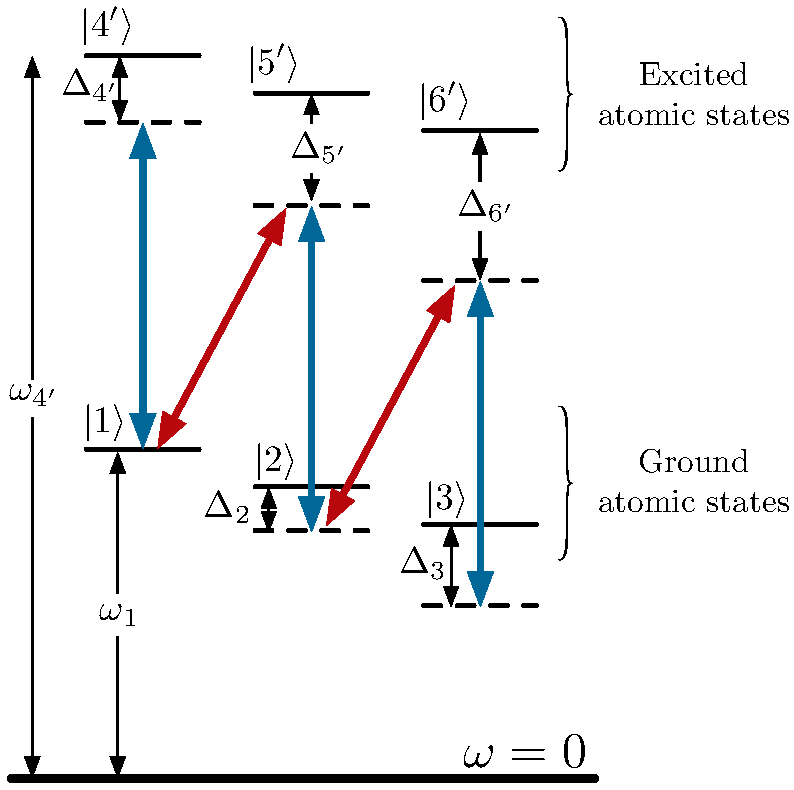
\includegraphics[width=6cm]{PhaseRotationDefinition}
    \caption{Schematic level diagram illustrating the definitions of the detunings in \eqref{OpticalPumping:PhaseRotationDefinition}. The sign of all detunings illustrated are positive.}
    \label{OpticalPumping:PhaseRotationDefinition}
\end{figure}

The equations of motion for the slowly-varying fields are
\begin{subequations}
    \label{OpticalPumping:MeanFieldTemporallySlowlyVarying}
    \begin{align}
        \begin{split}
            i \hbar \frac{\partial}{\partial t} \widetilde{\Psi}_i(\vect{x}) &= \left( -\frac{\hbar^2 \nabla^2}{2M} + V_i(\vect{x}) + U \sum_j \abs{\widetilde{\Psi}_j(\vect{x})}^2 - \hbar \omega_{i} + \hbar \Delta_i \right) \widetilde{\Psi}_i(\vect{x}) \\
            &\relphantom{=} - \sum_{j',n} \vect{d}_{ij'} \cdot \unitvec{u}^*_{\lambda_n}(\vect{q}_n) \widetilde{E}_{+,\vect{q}_n}^*(\vect{x}) \widetilde{\Psi}_{j'}(\vect{x}) e^{-i \left[\omega_{j'} - \Delta_{j'} - (\omega_i - \Delta_i) - \omega_{\vect{q}_n}\right] t},
        \end{split}\\
        \begin{split}
            i \hbar \frac{\partial}{\partial t} \widetilde{\Psi}_{i'}(\vect{x}) &= \left( -\frac{\hbar^2 \nabla^2}{2M} + V_{i'}(\vect{x}) + U \sum_j \abs{\widetilde{\Psi}_j(\vect{x})}^2 - \frac{i\hbar \Gamma}{2} - \hbar \omega_{i'} + \hbar \Delta_{i'}\right) \widetilde{\Psi}_{i'}(\vect{x})\\
            &\relphantom{=} - \sum_{j,n} \vect{d}_{i'j} \cdot \unitvec{u}_{\lambda_n}(\vect{q}_n) \widetilde{E}_{+,\vect{q}_n}(\vect{x}) \widetilde{\Psi}_{j}(\vect{x})  e^{-i \left[\omega_{j} - \Delta_j - (\omega_{i'} - \Delta_{i'}) + \omega_{\vect{q}_n}\right]t},
        \end{split}\\
        \begin{split}
          \frac{1}{c} \frac{\partial}{\partial t} \widetilde{E}_{+, \vect{q}_n} (\vect{x}) &= - \unitvec{q}_n \cdot \nabla \widetilde{E}_{+, \vect{q}_n}(\vect{x}) + i \abs{\vect{q}_n} \widetilde{E}_{+, \vect{q}_n}(\vect{x})\\
          &\relphantom{=} + i \frac{\abs{\vect{q}_n}}{2 \varepsilon_0} \unitvec{u}^*_{\lambda_n}(\vect{q}_n) \cdot \sum_{\{i,j'\}\in T_n} \vect{d}_{ij'} \widetilde{\Psi}^*_i(\vect{x}) \widetilde{\Psi}_{j'}(\vect{x}) e^{-i \left[\omega_{j'} - \Delta_{j'} -(\omega_i - \Delta_i) - \omega_{\vect{q}_n}\right] t}.
        \end{split}
    \end{align}
\end{subequations}
If the level detunings are chosen such that all optical fields couple resonantly between the `detuned levels' (dotted lines in \figureref{OpticalPumping:PhaseRotationDefinition}), the arguments of the exponential terms in \eqref{OpticalPumping:MeanFieldTemporallySlowlyVarying} will all be zero and the terms themselves will be equal to $1$.  Stated mathematically this requirement is
\begin{align}
    \big(\omega_{j'} - \Delta_{j'}\big) - \big(\omega_i - \Delta_i\big) &= \omega_{\vect{q}_n} \;\forall \; i, j', n : \left\{i, j'\right\} \in T_n.
\end{align}
This requirement is satisfied by the optical pumping scheme (see \figureref{OpticalPumping:LevelDiagram}) as the pumping laser defines the detunings of the $F'$ states relative to the $F=2$ states, and the $\sigma^+$ light generated on the $\ket{F=1, m_F=-1} \leftrightarrow \ket{F'=1, m_F=0}$ transition is formed spontaneously, and will therefore be resonant with the transition from the (possibly detuned) $\ket{F'=1, m_F=0}$ state such that the overall two-photon process $\ket{F=2, m_F=0} \leftrightarrow \ket{F=1, m_F=-1}$ is resonant.

With the evolution equations for the slowly-varying envelopes obtained, we may now work to eliminate effects on the propagation timescale of the electric fields.  To achieve this, we choose an arbitrary electric field $\widetilde{E}_{+, \vect{q}_n}$  and transform our coordinate system according to
\begin{align}
  \vect{x}' &= \vect{x}, \\
  t' &= t - \frac{1}{c} \unitvec{q}_n \cdot \vect{x}.
\end{align}

In the primed coordinates, the propagation equation for $\widetilde{E}_{+, \vect{q}_n}$ is
\begin{align}
    \label{OpticalPumping:ElectricFieldSpatialPropagation}
  \begin{split}
    \unitvec{q}_n \cdot \nabla_{\vect{x}'} \widetilde{E}_{+, \vect{q}_n}(\vect{x}', t') &= i \abs{\vect{q}_n} \widetilde{E}_{+, \vect{q}_n}(\vect{x}', t')\\
    &\relphantom{=} + i \frac{\abs{\vect{q}_n}}{2 \varepsilon_0} \unitvec{u}^*_{\lambda_n}(\vect{q}_n) \cdot \sum_{\{i,j'\}\in T_n} \vect{d}_{ij'} \widetilde{\Psi}^*_i\left(\vect{x}', t(\vect{x}', t')\right) \widetilde{\Psi}_{j'}\left(\vect{x}', t(\vect{x}', t')\right),
  \end{split}
\end{align}
where $\widetilde{E}_{+, \vect{q}_n}$ is written as a function of $(\vect{x}', t')$, while the atomic fields are written as functions of $(\vect{x}, t)$.  Although the primed and unprimed time coordinates are not exactly equal, if the spatial origin is chosen to be in the centre of the condensate then $t(\vect{x}', t') \approx t'$ is a very good approximation.  We can estimate the size of the terms neglected by this approximation by considering the variation in the atomic fields over the time $t'-t$,
\begin{align}
    \widetilde{\Psi}^*_i\left(\vect{x}', t(\vect{x}', t')\right) &= \widetilde{\Psi}^*_i\left(\vect{x}', t' + \frac{1}{c} \unitvec{q}_n \cdot \vect{x} \right), \notag\\
    &\approx \widetilde{\Psi}^*_i(\vect{x}', t') \left(1 + i  \frac{\delta \omega}{c}\unitvec{q}_n \cdot \vect{x} \right),
\end{align}
where the atomic field $\widetilde{\Psi}_{i}$ is assumed to evolve in time as $e^{-i\, \delta\omega\, t}$ for sufficiently small times.  For a condensate of maximum spatial extent $\sim \unit[100]{\micro m}$ and an excitation frequency $\delta \omega\sim \unit[10^5]{rad\,s\textsuperscript{-1}}$ (of the order of the chemical potential; refer to the discussion at the end of \sectionref{Peaks:ElementaryExcitations}), this correction term is of the order of
\begin{align}
    \abs{\delta \widetilde{\Psi} / \widetilde{\Psi}} &\leq \frac{\unit[100]{\micro m} \times \unit[10^{5}]{rad\,s\textsuperscript{-1}}}{3 \times \unit[10^8]{m\,s\textsuperscript{-1}}} \approx 10^{-7}.
\end{align}
Although neglecting this correction term is a zeroth-order approximation, the term being neglected is sufficiently small to make this approximation as good as (or better than) many of the first-order approximations that are made elsewhere in this derivation.  A similar approximation needs to be made in the evolution equations for the atomic fields (written in the unprimed coordinate system), $\widetilde{E}_{+, \vect{q}_n}(\vect{x}, t) \approx \widetilde{E}_{+, \vect{q}_n}(\vect{x}, t')$ with a similarly-sized correction.  

The overall effect of this change of coordinate system has been to neglect the temporal derivative in the evolution equation for the electric field mode $\widetilde{E}_{+, \vect{q}_n}$.  To the same degree of approximation, the temporal derivatives of all other electric field modes may also therefore be neglected.  These approximations made, the equations of motion become
\begin{subequations}
    \begin{align}
        \begin{split}
            i \hbar \frac{\partial}{\partial t} \widetilde{\Psi}_i(\vect{x}) &= \left( -\frac{\hbar^2 \nabla^2}{2M} + V_i(\vect{x}) + U \sum_j \abs{\widetilde{\Psi}_j(\vect{x})}^2 - \hbar \omega_{i} + \hbar \Delta_i \right) \widetilde{\Psi}_i(\vect{x})\\
            &\relphantom{=} - \sum_{j',n} \vect{d}_{ij'} \cdot \unitvec{u}^*_{\lambda_n}(\vect{q}_n) \widetilde{E}_{+,\vect{q}_n}^*(\vect{x}) \widetilde{\Psi}_{j'}(\vect{x}),
        \end{split}\\
        \begin{split}
            i \hbar \frac{\partial}{\partial t} \widetilde{\Psi}_{i'}(\vect{x}) &= \left( -\frac{\hbar^2 \nabla^2}{2M} + V_{i'}(\vect{x}) + U \sum_j \abs{\widetilde{\Psi}_j(\vect{x})}^2 - \frac{i\hbar \Gamma}{2} - \hbar \omega_{i'} + \hbar \Delta_{i'}\right) \widetilde{\Psi}_{i'}(\vect{x})\\
            &\relphantom{=} - \sum_{j,n} \vect{d}_{i'j} \cdot \unitvec{u}_{\lambda_n}(\vect{q}_n) \widetilde{E}_{+,\vect{q}_n}(\vect{x}) \widetilde{\Psi}_{j}(\vect{x}),
        \end{split} \label{OpticalPumping:AtomicExcitedStateEvolution}\\
      \unitvec{q}_n \cdot \nabla \widetilde{E}_{+, \vect{q}_n}(\vect{x}) &= i \abs{\vect{q}_n} \widetilde{E}_{+, \vect{q}_n}(\vect{x}) + i \frac{\abs{\vect{q}_n}}{2 \varepsilon_0} \unitvec{u}^*_{\lambda_n}(\vect{q}_n) \cdot \sum_{\{i,j'\}\in T_n} \vect{d}_{ij'} \widetilde{\Psi}^*_i\left(\vect{x}\right) \widetilde{\Psi}_{j'}\left(\vect{x}\right),
    \end{align}
\end{subequations}
where boundary values for the $\widetilde{E}_{+, \vect{q}_n}$ over a plane perpendicular to $\unitvec{q}_n$ must be specified to complete the system of equations.  With the temporal derivatives of the evolution equations for the electric fields neglected, these equations need to be solved self-consistently at every time point.  When all electric fields are propagating in the same direction, the evolution of the electric fields is an initial-value problem propagating in the $\unitvec{q}_n$ direction.  This is not the case in the optical pumping scheme in which optical modes may propagate both upwards and downwards.  However as the electric fields evolve slowly in time, the self-consistent solutions may be found iteratively starting from the solution found for the previous time point.

After eliminating the light propagation timescale from the problem, the next fastest timescale is that of the excited atomic states $\widetilde{\Psi}_{i'}$.  The evolution of these states is dominated either by spontaneous decay at a rate $\Gamma = 2\pi \times \unit[5.9]{MHz}$ or by the detuning term (if the pumping laser is detuned by several linewidths).  As these frequencies are much higher than the slower atomic evolution we are interested in ($\sim\unit[10]{kHz}$), the excited states may be adiabatically eliminated.  

To adiabatically eliminate the excited atomic states, we first recognise that the $\hbar \omega_{i'}$ term in \eqref{OpticalPumping:AtomicExcitedStateEvolution} will approximately balance the kinetic, potential and mean-field terms.  With this cancellation made, the adiabatic elimination of the excited atomic states can be made by setting the temporal derivative to zero yielding
\begin{align}
    \widetilde{\Psi}_{i'}(\vect{x}) &\approx \sum_{j, n} \frac{ \vect{d}_{i' j}\cdot \unitvec{u}_{\lambda_n}(\vect{q}_n) \widetilde{E}_{+, \vect{q}_n}(\vect{x}) \widetilde{\Psi}_j(\vect{x})}{\hbar \Delta_{i'} - \frac{i \hbar}{2}\Gamma}.
\end{align}
Substituting this expression back into the remaining evolution equations gives
\begin{subequations}
    \label{OpticalPumping:GeneralMultimodeModel}
    \begin{align}
        \begin{split}
            i \hbar \frac{\partial}{\partial t} \widetilde{\Psi}_i(\vect{x}) &= \left( -\frac{\hbar^2 \nabla^2}{2M} + V_i(\vect{x}) + U \sum_j \abs{\widetilde{\Psi}_j(\vect{x})}^2 - \hbar \omega_{i} + \hbar \Delta_i \right) \widetilde{\Psi}_i(\vect{x})\\
            &\relphantom{=} - \sum_{\substack{j',n\\ l,m}}  \frac{ \left[\vect{d}_{ij'} \cdot \unitvec{u}^*_{\lambda_n}(\vect{q}_n) \right]\left[\vect{d}_{j'l} \cdot \unitvec{u}_{\lambda_m}(\vect{q}_m)\right] }{\hbar \Delta_{j'} - \frac{i \hbar}{2}\Gamma} \widetilde{E}_{+,\vect{q}_n}^*(\vect{x}) \widetilde{E}^{\phantom{*}}_{+, \vect{q}_m}(\vect{x}) \widetilde{\Psi}_{l}(\vect{x}),
        \end{split}\\
        \begin{split}
            \unitvec{q}_n \cdot \nabla \widetilde{E}_{+, \vect{q}_n}(\vect{x}) &= i \abs{\vect{q}_n} \widetilde{E}_{+, \vect{q}_n}(\vect{x}) \\
            &\relphantom{=} + i \frac{\abs{\vect{q}_n}}{2 \varepsilon_0} \sum_{\substack{\{i,j'\}\in T_n\\ l, m}} \frac{\left[\vect{d}_{ij'}\cdot\unitvec{u}^*_{\lambda_n}(\vect{q}_n)\right] \left[\vect{d}_{j' l}\cdot \unitvec{u}_{\lambda_m}(\vect{q}_m)\right] }{\hbar \Delta_{j'} - \frac{i \hbar}{2}\Gamma}  \widetilde{\Psi}^*_i(\vect{x}) \widetilde{\Psi}_l(\vect{x}) \widetilde{E}_{+, \vect{q}_m}(\vect{x}).
        \end{split}
    \end{align}
\end{subequations}
This set of equations for the ground state atomic modes and the optical modes they interact with represents the basic multimode model that will be used in the remainder of this chapter.

\parasep

Several approximations were made in deriving the model derived in this section.  A summary of the most significant approximations is given below.
\begin{itemize}
    \item Scattering of spontaneously emitted photons has been neglected.  While this process can be neglected if the pumping laser is sufficiently detuned from resonance, this is potentially a significant issue closer to resonance.  As discussed in \sectionref{OpticalPumping:PumpingMechanism}, reabsorption can be negligible when operating in the boson accumulation regime in which excited atoms are significantly more likely to decay into the condensate mode than into all other modes.  It is this regime in which the continuous pumping experiment is operated.
    \item Atoms that have undergone spontaneous emission are neglected.  These thermal atoms will contribute to collisional heating of the condensate.  Provided that they are small in number compared to the condensate this heating can be neglected.  For a continuously pumped atom laser this requires that more atoms are transferred to the condensate than are lost due to spontaneous emission.
    \item Various time- and length-scales have been neglected.  The results of the model are only valid for timescales greater than the spontaneous lifetime of the system $\sim \unit[27]{ns}$, and for lengthscales larger than the optical wavelength $\lambda = \unit[780]{nm}$.
\end{itemize}

In the following sections the multimode pumping model derived here will be applied to some idealised systems to further investigate the pumping mechanism before considering the pumping experiment itself.

\subsection{Two overlapping condensates model}
\label{OpticalPumping:SimpleModels:OverlappingCondensatesModel}

\begin{figure}
    \centering
    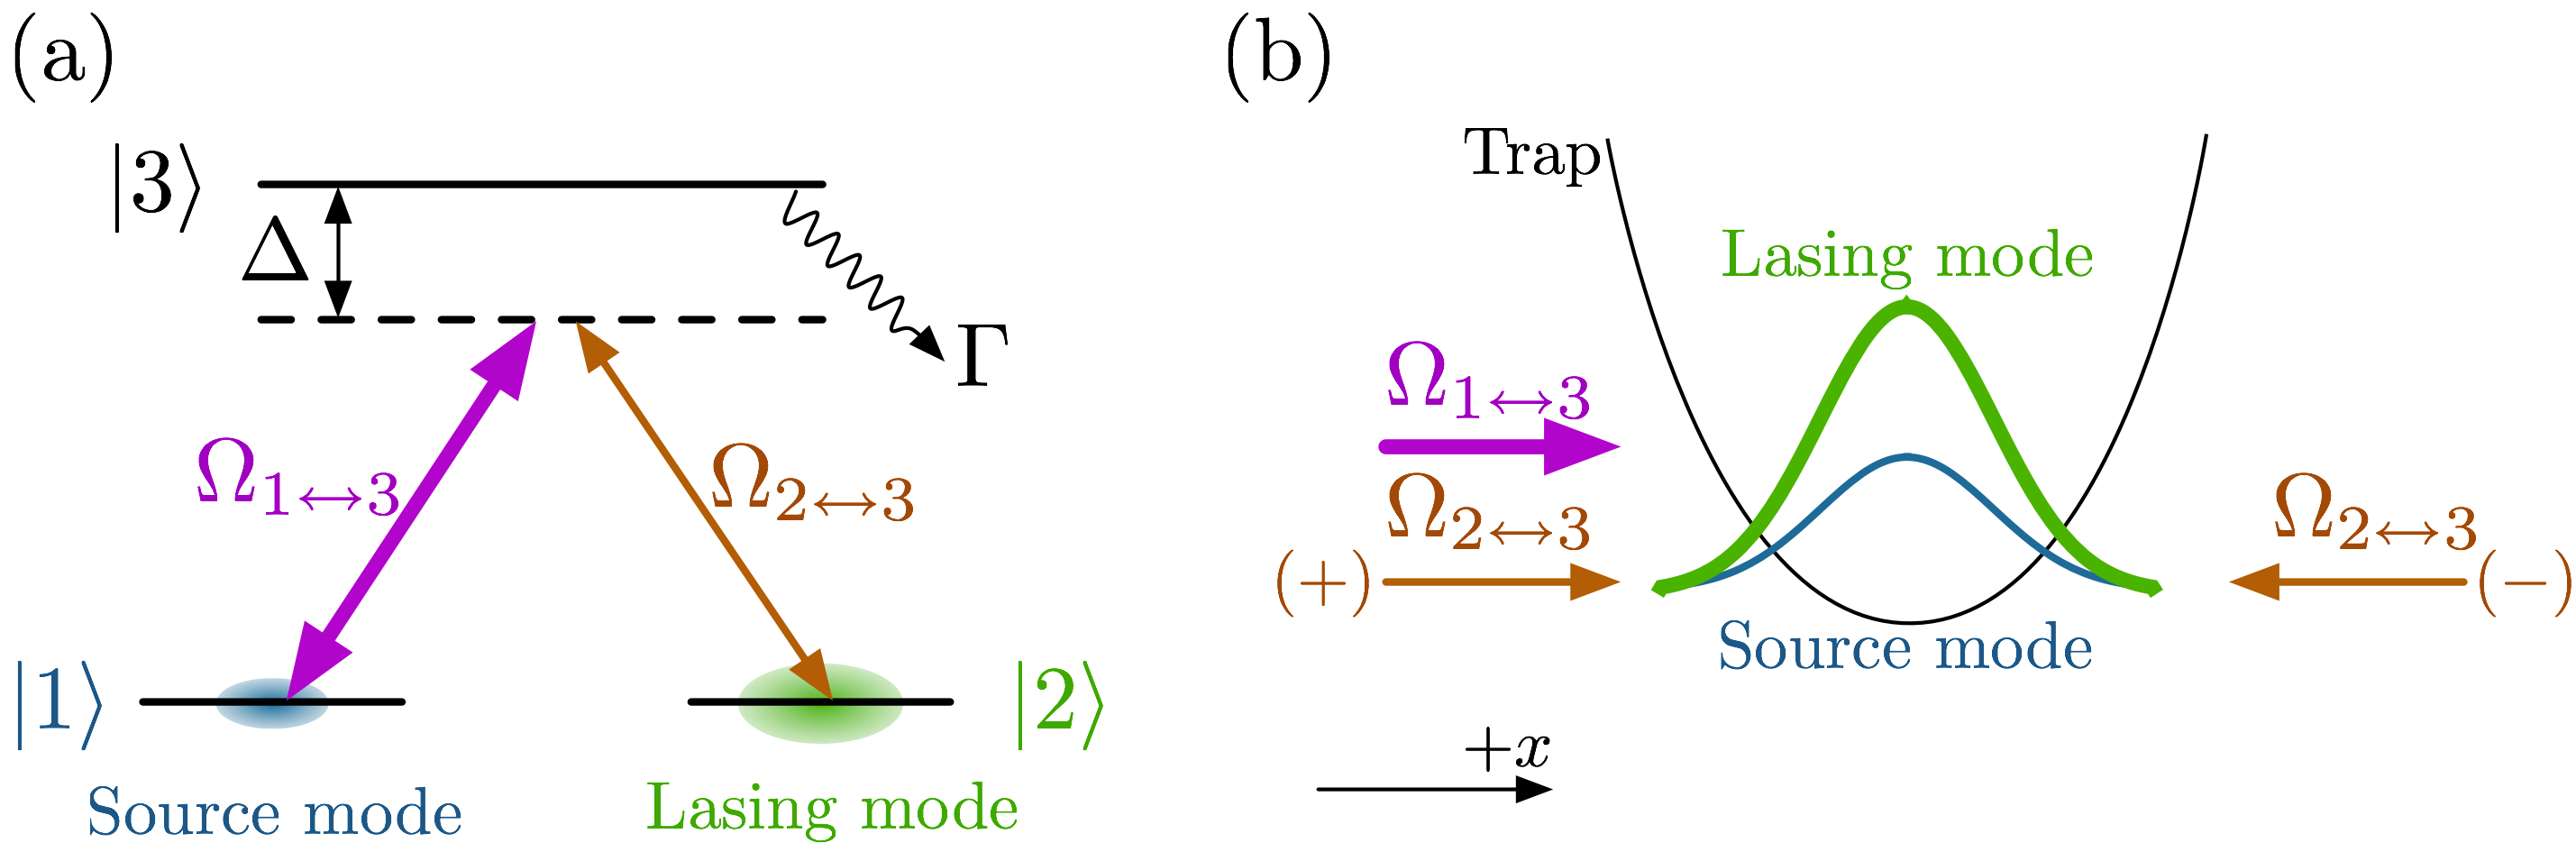
\includegraphics[width=14cm]{OverlappingCondensateModel}
    \caption{Schematic of the two overlapping condensates model.  The system consists of two condensates in the two ground states of a $\Lambda$ level scheme (a).  The system is illuminated on the $\ket{1}\leftrightarrow\ket{3}$ transition by light at a detuning $\Delta$ and Rabi frequency $\Omega_{1\leftrightarrow 3}$.  Light on the $\ket{2} \leftrightarrow \ket{3}$ transition is generated as atoms in the $\ket{3}$ state are stimulated to emit into the lasing mode $\ket{2}$.  Depending on the relative momenta of the atoms in the source and lasing modes, the light on the $\ket{2} \leftrightarrow \ket{3}$ transition will travel to the left or right.  The `$+$' sign in \eqref{OpticalPumping:OverlappingCondensatesEvolution:Omega2} corresponds to the optical field $\Omega_{2\leftrightarrow 3}$ propagating to the right [marked with $(+)$], while the `$-$' sign corresponds to propagation to the left [marked with $(-)$].}
    \label{OpticalPumping:OverlappingCondensateModel}
\end{figure}

The first idealised (multimode) pumping model to be considered is a simplified model of the transfer process occurring at the centre of the lasing condensate in the continuous pumping experiment.  In this model, illustrated in \figureref{OpticalPumping:OverlappingCondensateModel}, the source and lasing modes are the two ground states ($\ket{1}$ and $\ket{2}$ respectively) of atoms with a $\Lambda$-level scheme.  Light on the $\ket{1} \leftrightarrow \ket{3}$ transition is applied with detuning $\Delta$ from the left with an initial Rabi frequency of $\Omega_{1\leftrightarrow 3}(-\infty)$.  Light on the $\ket{2} \leftrightarrow \ket{3}$ transition is not supplied externally but may be produced as a result of atoms in the excited state ($\ket{3}$) being stimulated to emit into the lasing mode ($\ket{2}$).  To investigate possible differences in behaviour if the two optical modes are co-propagating or counter-propagating, we will consider both the case in which the source mode is initially stationary (with the $\Omega_{2\leftrightarrow 3}$ mode propagating to the right) and moving to the left with momentum $2 \hbar k$ (with the $\Omega_{2\leftrightarrow 3}$ mode propagating to the left).  In both cases the initial condition is chosen such that the lasing and source modes are in the overall ground state of the system given their respective initial occupations $N_\text{lasing}(t=0)$ and $N_\text{source}(t=0)$ (i.e.\  in the absence of any optical coupling the system would remain static).  The source mode is assumed to be given its momentum kick to the left (if appropriate) immediately before the optical field $\Omega_{1\leftrightarrow 3}$ is turned on at $t=0$.  As the $\Omega_{2\leftrightarrow 3}$ light is generated by (atomic) stimulated emission its phase will be determined by the phase difference between the source and lasing modes, we may assume there to be a specific phase relationship between the two modes without loss of generality; our results will also apply if the two condensates were independently produced and had a random relative phase.

For the 1D scheme presented in \figureref{OpticalPumping:OverlappingCondensateModel} we may simplify the multimode equations \eqref{OpticalPumping:GeneralMultimodeModel} to
\begin{subequations}
    \label{OpticalPumping:OverlappingCondensatesEvolution}
    \begin{align}
        \begin{split}
            i \hbar \frac{\partial}{\partial t} \Psi_1(x) &= \left[- \frac{\hbar^2}{2M}\frac{d^2}{dx^2} + V_\text{trap}(x) + U_\text{1D}\left(\abs{\Psi_1}^2 + \abs{\Psi_2}^2\right)  \right] \Psi_1\\
            &\relphantom{=} - \hbar \frac{\abs{\Omega_{1\leftrightarrow 3}}^2\Psi_1 + \Omega_{1\leftrightarrow 3}^* \Omega_{2\leftrightarrow 3}^{\phantom{*}}\Psi_2}{\Delta - \frac{i}{2} \Gamma},
        \end{split} \label{OpticalPumping:OverlappingCondensatesEvolution:Psi1}\\
        \begin{split}
            i \hbar \frac{\partial}{\partial t} \Psi_2(x) &= \left[- \frac{\hbar^2}{2M}\frac{d^2}{dx^2} + V_\text{trap}(x) + U_\text{1D}\left(\abs{\Psi_1}^2 + \abs{\Psi_2}^2\right)  \right] \Psi_2\\
            &\relphantom{=} - \hbar \frac{\abs{\Omega_{2\leftrightarrow 3}}^2 \Psi_2 + \Omega_{2\leftrightarrow 3}^* \Omega_{1\leftrightarrow 3}^{\phantom{*}} \Psi_1}{\Delta - \frac{i}{2} \Gamma},
        \end{split} \label{OpticalPumping:OverlappingCondensatesEvolution:Psi2}\\
        \frac{d}{dx} \Omega_{1\leftrightarrow 3} &= i k \Omega_{1\leftrightarrow 3} + \frac{i}{4} f_{13} \Gamma \frac{\sigma_0}{A_\perp} \frac{\abs{\Psi_1}^2 \Omega_{1\leftrightarrow 3} + \Psi_1^* \Psi_2^{\phantom{*}}\Omega_{2\leftrightarrow 3}}{\Delta - \frac{i}{2} \Gamma}, \label{OpticalPumping:OverlappingCondensatesEvolution:Omega1}\\
        \pm \frac{d}{dx} \Omega_{2\leftrightarrow 3} &= i k \Omega_{2\leftrightarrow 3} + \frac{i}{4} f_{23} \Gamma \frac{\sigma_0}{A_\perp} \frac{\abs{\Psi_2}^2 \Omega_{2\leftrightarrow 3} + \Psi_2^* \Psi_1^{\phantom{*}} \Omega_{1\leftrightarrow 3}}{\Delta - \frac{i}{2} \Gamma}, \label{OpticalPumping:OverlappingCondensatesEvolution:Omega2}
    \end{align}
\end{subequations}
where the electric fields of \eqref{OpticalPumping:GeneralMultimodeModel} have been replaced with Rabi frequencies\footnote{Electric fields must be used in the general case in which a single optical field may couple multiple transitions with different dipole matrix elements.  In the present model each optical field drives only a single transition, enabling the electric fields to be replaced with Rabi frequencies.} using $\hbar \Omega_i = \vect{d}_{i 3} \cdot \unitvec{u}_{\lambda_i} \widetilde{E}_{+, \vect{q}_i}$; the remaining dipole matrix elements have been eliminated in favour of the spontaneous emission rate using $\displaystyle \Gamma = \frac{\omega^3 d_\text{total}^2}{3 \pi \epsilon_0 \hbar c^3}$, where the total dipole matrix element is $\abs{d_\text{total}}^2 = \sum_{i} \abs{\vect{d}_{i3}}^2$ with $\abs{\vect{d}_{i3}}^2 = f_{i3} \abs{d_\text{total}}^2$, where $f_{i3}$ is the fraction of atoms in the $\ket{3}$ state that decay to the $\ket{i}$ state; $\displaystyle\sigma_0 = \frac{3 \lambda^2}{2 \pi}$ is the atomic scattering cross-section; and a very simple dimension reduction scheme has been used: $\Psi_i^\text{(3D)} = \Psi_i^\text{(1D)} / \sqrt{A_\perp}$, $U_\text{1D} = U_\text{3D} / A_\perp$, where $A_\perp$ is a representative area of the condensate perpendicular to the $x$ direction.  The positive sign in \eqref{OpticalPumping:OverlappingCondensatesEvolution:Omega2} applies if the source mode is initially stationary causing the $\Omega_{2\leftrightarrow 3}$ mode to propagate to the right, and the negative sign applies if the source mode is initially moving to the left with momentum $2 \hbar k$ causing the $\Omega_{2\leftrightarrow 3}$ mode to propagate to the left.

Before simulating the system numerically, some analytical insight can be obtained by considering the behaviour of the optical fields as they propagate through the condensates.  Although propagating in space instead of in time, the equations of motion for the optical fields resemble those for a coupled $\Lambda$ level scheme with the \emph{atomic} fields governing the strength of the coupling of each transition, a role normally filled by optical fields.  Rewriting the evolution equations for the two optical fields elucidates this analogy,
\begin{subequations}
    \label{OpticalPumping:OpticalPropagationAnalogy}
    \begin{align}
        i \hbar c \frac{d}{dx} \phi_{1\leftrightarrow 3} &= -\hbar \omega \phi_{1\leftrightarrow 3}  - \hbar \frac{\abs{\Omega_1}^2 \phi_{1\leftrightarrow 3} + \Omega_1^* \Omega_2^{\phantom{*}} \phi_{2\leftrightarrow 3}}{\Delta - \frac{i}{2} \Gamma},\\
        \pm i \hbar c\frac{d}{dx} \phi_{2\leftrightarrow 3} &= - \hbar \omega \phi_{2\leftrightarrow 3} - \hbar \frac{\abs{\Omega_2}^2 \phi_2 + \Omega_2^* \Omega_1^{\phantom{*}} \phi_{1\leftrightarrow 3}}{\Delta - \frac{i}{2} \Gamma},
    \end{align}
\end{subequations}
where $\displaystyle\Omega_i = \sqrt{\frac{c \Gamma \sigma_0}{8 A_\perp}} \Psi_i$, $\phi_{i\leftrightarrow j}$ has been used to replace the optical Rabi frequencies $\Omega_{i \leftrightarrow j}$ to limit the possibility for confusion, and it has been assumed that the two optical transitions are of equal strength, hence $f_{13} = f_{23} = \frac{1}{2}$.  The coupling terms between the two fields $\phi_{1 \leftrightarrow 3}$ and $\phi_{2 \leftrightarrow 3}$ are now clearly in the same form as the atomic coupling terms between $\Psi_1$ and $\Psi_2$ in \eqref{OpticalPumping:OverlappingCondensatesEvolution:Psi1}--\eqref{OpticalPumping:OverlappingCondensatesEvolution:Psi2}.  This similarity is not surprising as the ground state atomic fields and the optical fields may be interchanged in the atom--light coupling Hamiltonian (after making the rotating-wave approximation) without changing its form:
\begin{align}
    \hat{H}_\text{atom--light} &\propto \hat{\Psi}_e^\dagger \hat{\Psi}_g^{\phantom{\dagger}} \hat{\phi} + \hat{\phi}^\dagger \hat{\Psi}_g^\dagger \hat{\Psi}_e^{\phantom{\dagger}},
\end{align}
where $\hat{\Psi}_e$, $\hat{\Psi}_g$ are the excited and ground atomic fields respectively and $\hat{\phi}$ is the photon field.

\begin{figure}
    \centering
    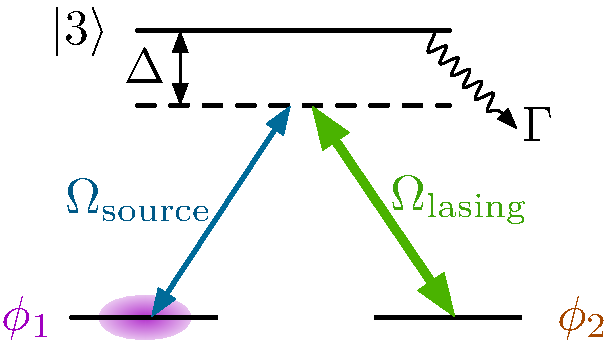
\includegraphics[width=6cm]{DualModel}
    \caption{The propagation of the photons through the system is analogous to Rabi flopping between two states in a $\Lambda$-level scheme.  The flopping between the two modes is driven by `Rabi frequencies' due to the atomic populations of the source and lasing modes.}
    \label{OpticalPumping:DualModel}
\end{figure}

This analogy for the photon propagation is illustrated in \figureref{OpticalPumping:DualModel}.  In this model the two fields $\phi_{1\leftrightarrow 3}$ and $\phi_{2 \leftrightarrow 3}$ are coupled by two Rabi frequencies $\Omega_1$ and $\Omega_2$ that vary (in space) as the two fields $\phi_{i \leftrightarrow j}$ evolve (in space).  For the counter-propagating case the analogy is imperfect as one mode propagates forward while the other backward, preventing a direct analogy with propagation in time.  For the co-propagating case however, the analogy is perfect and the optical propagation equations can be solved exactly for small times while the source and lasing modes have the same shape.  The solution for $\Omega_{2\leftrightarrow 3}$ is
\begin{align}
    \Omega_{2\leftrightarrow 3}(x) &= \Omega_{1\leftrightarrow 3}(-\infty) \frac{\Psi_1^{\phantom{*}} \Psi_2^*}{\abs{\Psi_1}^2 + \abs{\Psi_2}^2} \left[\exp \left( i \frac{\Gamma \sigma_0}{8 A_\perp\left(\Delta - \frac{i}{2} \Gamma\right)}\int_{-\infty}^x dx\, \abs{\Psi_1}^2 + \abs{\Psi_2}^2\right) -1 \right].
\end{align}

As every photon that leaves the system in the $\Omega_{2\leftrightarrow 3}$ optical mode corresponds to an atom being transferred into the lasing mode, the net rate of atom transfer will be governed by
\begin{align}
    \abs{\Omega_{2\leftrightarrow 3}(+\infty)}^2 &= \abs{\Omega_{1\leftrightarrow 3}(-\infty)}^2 \frac{N_1}{N} \frac{N_2}{N} \abs{\alpha - 1}^2, \label{OpticalPumping:OverlappingCondensates:Omega2Infinity}
\end{align}
where
\begin{align}
    \alpha &= \exp \left( i \frac{N\Gamma \sigma_0}{8 A_\perp\left(\Delta - \frac{i}{2} \Gamma\right)}\right),
\end{align}
$N_i$ is the number of atoms in the $\ket{i}$ state, and $N = N_1 + N_2$ is the number of atoms in the system.  

The rate of atom transfer into the lasing mode is then
\begin{align}
    \frac{d N_2}{dt} &= \abs{\Omega_{2\leftrightarrow 3}(+\infty)}^2 \frac{8 A_\perp}{\Gamma \sigma_0} \\
     &= \abs{\Omega_{1\leftrightarrow 3}(-\infty)}^2 \frac{8 A_\perp}{\Gamma \sigma_0} \frac{N_1}{N} \frac{N_2}{N} \abs{\alpha - 1}^2. \label{OpticalPumping:OverlappingCondensates:TransferRate}
\end{align}
The rate of atom transfer out of the source mode can be found in a similar way.  From these two rates the efficiency of the pumping process may be obtained,
\begin{align}
    \eta &= \left.\frac{d N_2}{d t} \middle / \left(- \frac{d N_1}{dt}\right)\right. = \frac{N_2 \abs{\alpha - 1}^2}{2 N \left(1 - \Re\{\alpha\}\right) - N_1 \abs{\alpha -1}^2}.
\end{align}

\subsubsection{Zero detuning limit ($\Delta = 0$)}

The continuous pumping experiment described in \sectionref{OpticalPumping:ContinuousExperiment} was operated with the pumping light resonant with the $\ket{F=2, m_F=0} \leftrightarrow \ket{F'=1, m_F=0}$ transition; the transition that is represented by the $\ket{1} \leftrightarrow \ket{3}$ transition in the present model.  It is therefore interesting to consider the zero detuning limit ($\Delta = 0$) as it would apply to the experiment.  Furthermore the the lasing mode (the $\ket{F=1, m_F=-1}$ condensate in the experiment) contains significantly more atoms than the source mode (the atom laser state $\ket{F=2, m_F=0}$), permitting the approximation $N_1 \ll N_2$.  

In these limits the parameter $\alpha$ becomes
\begin{align}
    \alpha &= \exp\left( - \frac{N \sigma_0}{4 A_\perp}\right) \approx \exp(- 121) \approx 0,
\end{align}
where a numerical value for $\alpha$ has been obtained using the experimentally-relevant values $\lambda = \unit[780]{nm}$, $N = 5 \times 10^5$, $A_\perp = 3\times\unit[10^{-10}]{m\textsuperscript{2}}$.  Using $\alpha \approx 0$ the transfer rate and efficiency take the simple forms:
\begin{align}
    \frac{d N_2}{dt} &\approx \abs{\Omega_{1\leftrightarrow 3}(-\infty)}^2 \frac{8 A_\perp}{\Gamma \sigma_0} \frac{N_1}{N_2}, \label{OpticalPumping:OverlappingCondensates:ZeroDetuningTransferRate}\\
    \eta &\approx \frac{N_2}{N + N_2} \approx \frac{1}{2} \label{OpticalPumping:OverlappingCondensates:ZeroDetuningEfficiency}.
\end{align}
As observed in the single-mode model of \sectionref{OpticalPumping:SingleModeModel} [see \eqref{OpticalPumping:SingleModePumpingRateZeroDetuning}], the transfer rate \emph{decreases} as the occupation of the lasing mode increases.  

An interesting difference with the single-mode model however is that the transfer efficiency in this model (for short times) cannot exceed 50\% while the efficiency of the single-mode model approaches 100\% for sufficiently large $N_2$.  This difference can be understood by recognising that the $\Lambda$ level scheme of \figureref{OpticalPumping:DualModel} has a dark eigenstate that does not undergo spontaneous emission as the $\ket{3}$ atomic state contains no population.  The dark eigenstate is
\begin{align}
    \ket{D} &= \frac{1}{\sqrt{\abs{\Psi_1}^2 + \abs{\Psi_2}^2}} \left(\Psi_2 \ket{1 \leftrightarrow 3}- \Psi_1 \ket{2\leftrightarrow 3}\right), \label{OpticalPumping:DarkState}\\
    &= \sqrt{\frac{N_2}{N}} \ket{1 \leftrightarrow 3} - \sqrt{\frac{N_1}{N}} \ket{2 \leftrightarrow 3} \label{OpticalPumping:DarkStateShortTimes}
\end{align}
where $\ket{i \leftrightarrow j}$ is the state for the optical mode resonant with the $\ket{i} \leftrightarrow \ket{j}$ transition.  When the optical modes are in this dark eigenstate, the numerators of the atom--light coupling terms of \eqref{OpticalPumping:OverlappingCondensatesEvolution} are zero.  The second form of the dark state \eqref{OpticalPumping:DarkStateShortTimes} only applies for short times while the two atomic modes have the same spatial profile (and assuming they have the same phase).  It is only the component that is in the dark state that will propagate through the system; all other components will be absorbed rapidly.  Although the projection of the initial (optical) state $\ket{\Psi_\text{initial}} = \ket{1 \leftrightarrow 3}$ onto the dark state
\begin{align}
    \abs{\braket{D}{\Psi_\text{initial}}}^2 &= \frac{N_2}{N}
\end{align}
may approach 1 arbitrarily, the efficiency only approaches $\frac{1}{2}$,
\begin{align}
    \eta &= \frac{\abs{\braket{2 \leftrightarrow 3}{D} \!\!\braket{D}{\Psi_\text{initial}}}^2}{1 - \abs{\braket{1 \leftrightarrow 3}{D} \!\! \braket{D}{\Psi_\text{initial}}}^2} = \frac{\frac{N_1}{N} \frac{N_2}{N}}{1 - \left(\frac{N_2}{N}\right)^2}, \notag\\
    &= \frac{N_2}{N + N_2} \approx \frac{1}{2},
\end{align}
in agreement with \eqref{OpticalPumping:OverlappingCondensates:ZeroDetuningEfficiency}.

The definition of the dark state \eqref{OpticalPumping:DarkState} suggests a method of improving this efficiency: if the profiles of the source and lasing modes are not the same but instead the $\Omega_{1\leftrightarrow 3}$ pumping beam first encounters atoms in the lasing mode before atoms in the source mode, the initial projection onto the dark state will be perfect.  If the variation of the source and lasing mode densities occurs over length scales significantly larger than the absorption length scale for the non-dark states ($\displaystyle d = \frac{4 A_\perp}{\sigma_0 \abs{\Psi_2}^2} \sim \unit[60]{nm}$), then the dark state will be followed adiabatically with minimal losses.  This situation will arise naturally at later times as the source atoms closest to the pumping beam are transferred to the lasing mode.  As this occurs, the pumping beam will encounter a greater proportion of atoms in the lasing mode than at earlier times thus increasing the efficiency.  This behaviour is observed numerically in simulations of the system \eqref{OpticalPumping:OverlappingCondensatesEvolution} as illustrated in \figureref{OpticalPumping:OverlappingCondensatesZeroDetuning}.

\begin{figure}
    \centering
    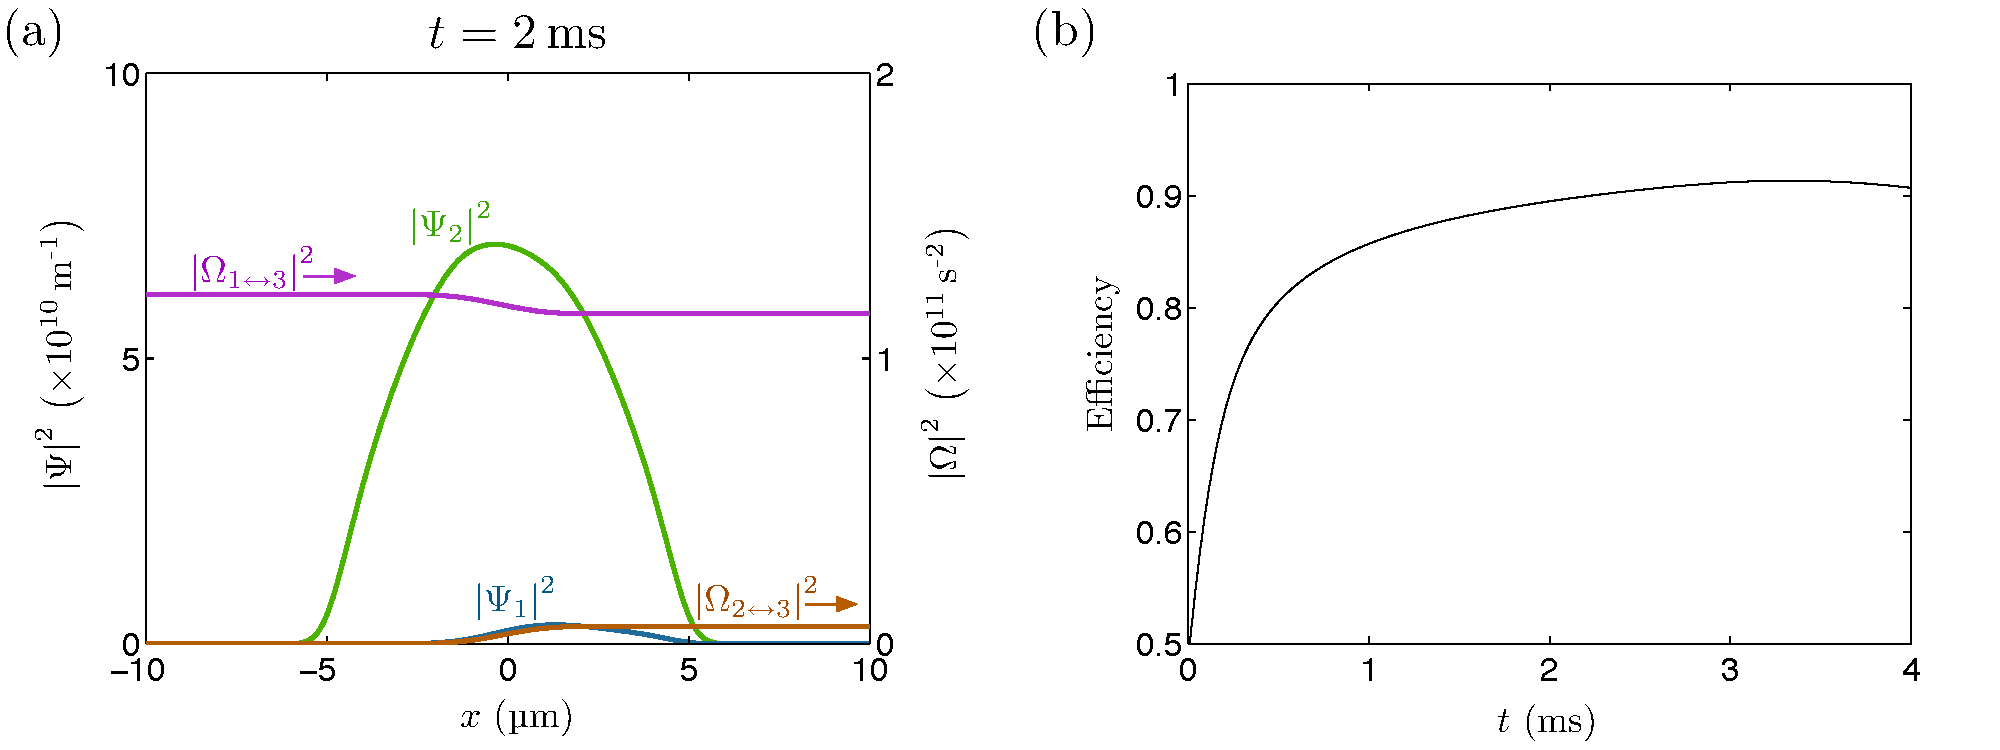
\includegraphics[width=15cm]{OverlappingCondensatesZeroDetuning}
    \caption{Simulation results of the two overlapping condensates model \eqref{OpticalPumping:OverlappingCondensatesEvolution} driven resonantly.  Figure (a) is a snapshot of the densities and magnitudes of the Rabi frequencies at $t = \unit[2]{ms}$.  The instantaneous efficiency is shown in (b).  There are a total of $N = 5 \times 10^5$ atoms in the system, of which initially 5\% are in the source mode ($\ket{1}$), and the system is driven resonantly with $\Omega_{1\leftrightarrow 3}(-\infty) = 3.5 \times \unit[10^5]{s\textsuperscript{-1}}$.}
    \label{OpticalPumping:OverlappingCondensatesZeroDetuning}
\end{figure}

While the efficiency of the population transfer is related to the leading edge of the density profiles, the rate of transfer can be related to the trailing edge.  The fraction of the photons leaving the system in the $\Omega_{2\leftrightarrow 3}$ mode is determined by the dark state at the trailing edge
\begin{align}
    \abs{\Omega_{2\leftrightarrow 3}(+\infty)}^2 &= \abs{\Omega_{1\leftrightarrow 3}(-\infty)}^2 \abs{\braket{2 \leftrightarrow 3}{D_\text{trailing}}\!\! \braket{D_\text{leading}}{\Psi_\text{initial}}}^2, \\
    &= \abs{\Omega_{1\leftrightarrow 3}(-\infty)}^2 \frac{N_1}{N} \frac{N_2}{N},
\end{align}
where the second equality only applies for short times while the two atomic modes have the same spatial profile, and is in agreement with \eqref{OpticalPumping:OverlappingCondensates:Omega2Infinity} as $\alpha \approx 0$.  The rate of population transfer can therefore be increased by having the dark state at the trailing edge to be almost purely the $\ket{2 \leftrightarrow 3}$ state.  This would be achieved by having the density in the lasing mode decay first before the density in the source mode.  In this limit, every photon in the pumping beam would transfer one atom into the lasing mode.  This possibility is related to the idea of adiabatic population transfer \citep{Kuklinski:1989}, and is investigated further in \sectionref{OpticalPumping:SimpleModels:AtomLaserModel}.


This system still suffers from the same problem discussed at the end of \sectionref{OpticalPumping:SingleModeModel}, i.e.\ that the transfer rate is lower than the spontaneous emission rate for atoms that are not momentum resonant with the lasing condensate.  If there is a non-zero time for which the source atoms are not resonant with the lasing condensate (for example, if they must fall from an upper condensate to a lower condensate), this population loss will significantly reduce the overall efficiency of the transfer process.  One possible solution to this problem would be if the pumping process were operated such that every photon in the $\Omega_{1\leftrightarrow 3}$ mode left the system in the $\Omega_{2\leftrightarrow 3}$ mode which the source atoms do not absorb.  This possibility is discussed further in \sectionref{OpticalPumping:SimpleModels:AtomLaserModel}.

\subsubsection{Far detuned limit ($\Delta \gg \Gamma$)}

Although the continuous pumping experiment described in \sectionref{OpticalPumping:ContinuousExperiment} was operated with resonant pumping light, the opposite limit is interesting due to the suppression of spontaneous emission.  In this limit the $\alpha$ parameter becomes
\begin{align}
    \alpha &= \exp\left( - \frac{N \sigma_0}{16 A_\perp} \frac{\Gamma^2}{\Delta^2 + \frac{1}{4}\Gamma^2}\right) \exp \left(i \frac{N \sigma_0}{8 A_\perp} \frac{\Gamma \Delta}{\Delta^2 + \frac{1}{4} \Gamma^2}\right) \\
    &\approx \exp \left( - \frac{N \sigma_0}{16 A_\perp} \frac{\Gamma^2}{\Delta^2}\right) \exp \left(i \frac{N \sigma_0}{8 A_\perp} \frac{\Gamma}{\Delta}\right) \\
    &\approx \exp \left( - 30 \frac{\Gamma^2}{\Delta^2}\right) \exp \left( 61 i \frac{\Gamma}{\Delta} \right) \label{OpticalPumping:FarDetunedLimit:ApproxAlphaNumerical},
\end{align}
where the same values have been used as in the resonant case.  Efficiencies close to unity require the magnitude of $\alpha$ to be close to 1.  While this can be achieved relatively easily (a detuning of a few 10's of linewidths is enough for the experimental parameters), the rate of population transfer depends strongly on the phase of $\alpha$ [see \eqref{OpticalPumping:OverlappingCondensates:TransferRate}].  If the detuning is not sufficiently large to make the phase of $\alpha$ small, the photons will Rabi flop between the $\ket{1 \leftrightarrow 3}$ and $\ket{2 \leftrightarrow 3}$ modes, reducing the rate of transfer into the lasing mode.  In this limit, the transfer rate into the lasing mode averaged over all phases for $\alpha$ is
\begin{align}
    \overline{\frac{d N_2}{dt}} &= \abs{\Omega_{1\leftrightarrow 3}(-\infty)}^2 \frac{16 A_\perp}{\Gamma \sigma_0} \frac{N_1}{N} \frac{N_2}{N} \approx \abs{\Omega_{1\leftrightarrow 3}(-\infty)}^2 \frac{16 A_\perp}{\Gamma \sigma_0} \frac{N_1}{N_2}, \label{OpticalPumping:OverlappingCondensates:IntermediateDetuningTransferRate}
\end{align}
which is twice that in the zero detuning limit \eqref{OpticalPumping:OverlappingCondensates:ZeroDetuningTransferRate}, and hence decreases as the occupation of the lasing mode increases.  The factor of two difference comes from the difference in efficiency: in this case the efficiency is approximately 100\%, while it is 50\% in the zero detuning limit.

The situation is much improved if the pumping light is sufficiently detuned that the phase of $\alpha$ is small.  In the limit
\begin{align}
    \frac{N \sigma_0}{8 A_\perp} \frac{\Gamma}{\Delta} &\ll 1,
\end{align}
the transfer rate is
\begin{align}
    \frac{d N_2}{dt} &\approx \frac{\abs{\Omega_{1\leftrightarrow 3}(-\infty)}^2}{\Delta} \frac{\sigma_0}{8 A_\perp} \frac{\Gamma}{\Delta} N_1 N_2, \label{OpticalPumping:OverlappingCondensates:FarDetuningTransferRate}
\end{align}
with an efficiency
\begin{align}
    \eta &\approx \left(1 + \frac{8 A_\perp}{N \sigma_0}\right)^{-1}.
\end{align}
The transfer rate for very high detunings displays Bose-enhancement as it increases for increasing occupation of the lasing mode.  This is a desirable property for a pumping mechanism, as it means that the highest-occupied mode will undergo more gain than lesser-occupied modes.  

As the transfer rate at high-detunings is Bose-enhanced, the system does not suffer from the same problem with spontaneous emission as exists closer to resonance.  The spontaneous emission rate of source atoms in the absence of the condensate,
\begin{align}
    \left. \frac{d N_1}{dt} \right|_\text{no condensate} &\approx - \frac{\abs{\Omega_{1\leftrightarrow 3}(-\infty)}^2}{\Delta^2}\Gamma N_1,
\end{align}
is significantly lower than the pumping rate in the presence of the lasing mode \eqref{OpticalPumping:OverlappingCondensates:FarDetuningTransferRate},
\begin{align}
    \left. \left. \frac{d N_2}{dt} \right|_\text{pumping} \middle / - \left. \frac{d N_1}{dt} \right|_\text{no condensate} \right. &\approx \frac{N \sigma_0}{8 A_\perp},
\end{align}
where this ratio is $\sim 60$ for the parameters of the continuous pumping experiment.

\subsubsection{Counter-propagating optical modes}
The behaviour of this system in the case that $\Omega_{1\leftrightarrow 3}$ and $\Omega_{2\leftrightarrow 3}$ are counter-propagating is not qualitatively different from that described previously for the co-propagating case.  This is because the pumping beam $\Omega_{1\leftrightarrow 3}$ cannot be significantly reduced by propagating through the system when the source mode is significantly less occupied than the lasing mode ($N_1 \ll N_2$).  After propagating through the system (in the co-propagating case), $\Omega_{1\leftrightarrow 3}$ is
\begin{align}
    \abs{\Omega_{1\leftrightarrow 3}(+\infty)}^2 &= \abs{\Omega_{1\leftrightarrow 3}(-\infty)}^2 \abs{1 + \frac{N_1}{N}\left(\alpha - 1\right)}^2.
\end{align}
For $N_1 \ll N$, $\Omega_{1\leftrightarrow 3}$ changes negligibly propagating through the system and is well approximated by a constant.  Being constant, its propagation direction relative to that of $\Omega_{2\leftrightarrow 3}$ can have little effect on the system's dynamics.  This is observed in simulations of \eqref{OpticalPumping:OverlappingCondensatesEvolution}.


\subsection{Simple atom laser model}
\label{OpticalPumping:SimpleModels:AtomLaserModel}

\begin{figure}
    \centering
    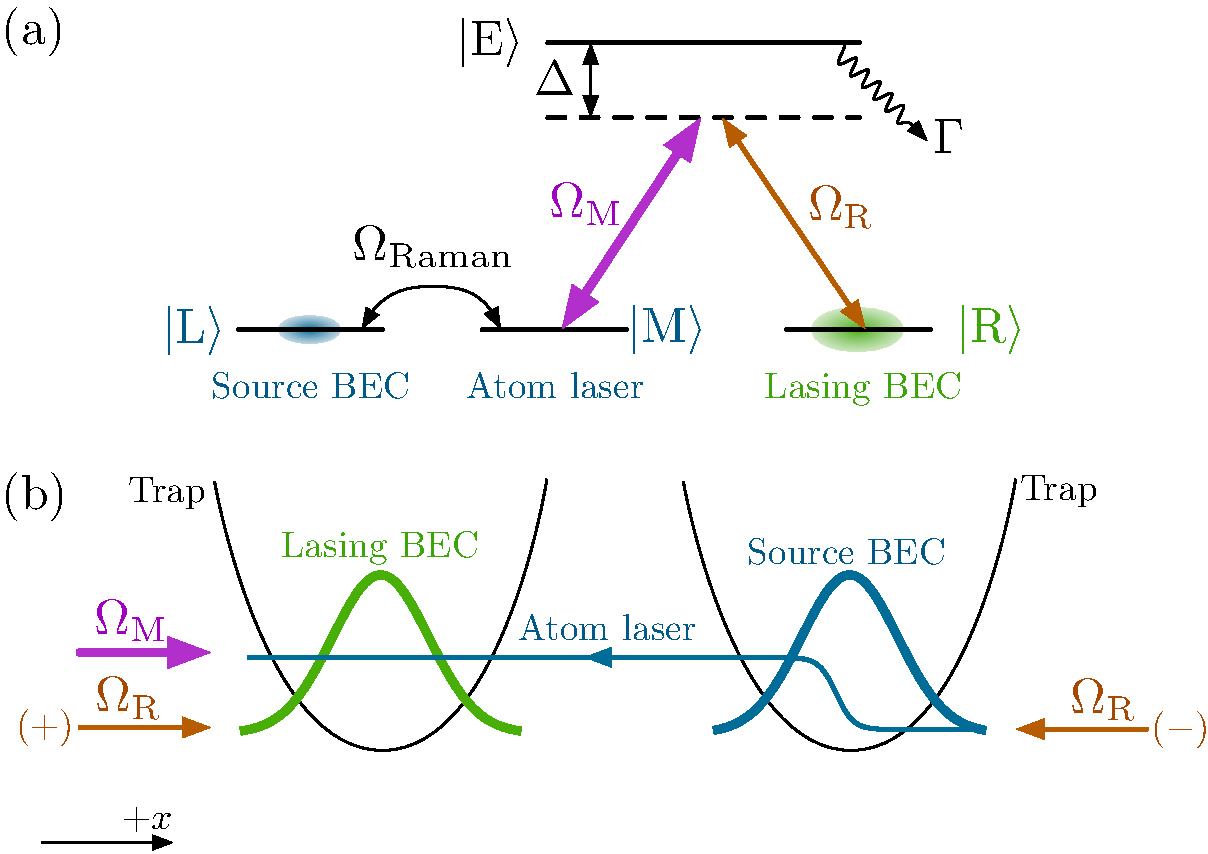
\includegraphics[width=12cm]{TravellingBeamModel}
    \caption{Schematic of the travelling beam model.  The additional excited level that is a necessary part of the Raman outcoupling process has been suppressed to simplify the diagram.  This scheme is governed by \eqref{OpticalPumping:TravellingBeamEvolution}.}
    \label{OpticalPumping:TravellingBeamModel}
\end{figure}

The previous model suggested that efficient population transfer with resonant light might be possible if the source and lasing modes partially overlap such that the first resonant atoms the pumping photons encounter are in the lasing mode and the last are in the source mode.  One way this might occur which is relevant to the continuous pumping experiment is illustrated in \figureref{OpticalPumping:TravellingBeamModel}.  In this model there are two trapped condensates, the source condensate $\ket{\text{S}}$, and the lasing condensate $\ket{\text{L}}$.  Atoms are outcoupled from the source condensate via a Raman transition to form an atom laser $\ket{\text{A}}$.  The Raman process gives atoms a $2 \hbar k$ momentum kick to the left as they are outcoupled from the source condensate.  The atom laser forms the source mode for the pumping process considered in the previous section (see \figureref{OpticalPumping:OverlappingCondensateModel}).  In this pumping process, light on the $\ket{A} \leftrightarrow \ket{\text{E}}$ transition is applied from the left with detuning $\Delta$ and an initial Rabi frequency of $\Omega_{\text{A}\leftrightarrow\text{E}}(-\infty)$.  Light on the $\ket{\text{L}} \leftrightarrow \ket{\text{E}}$ transition is produced as atoms in the excited state $\ket{\text{E}}$ are stimulated to emit into the lasing condensate $\ket{\text{L}}$.  Similarly to \sectionref{OpticalPumping:SimpleModels:OverlappingCondensatesModel}, we consider the cases in which the light on the $\ket{\text{L}} \leftrightarrow \ket{\text{E}}$ transition propagates from the right or the left.  Physically, only the case in which $\Omega_{\text{L}\leftrightarrow\text{E}}$ propagates from the right can be momentum resonant as the $2 \hbar k$ of momentum transferred in this process will cancel the momentum of the atoms in the atom laser.  The process in which $\Omega_{\text{L}\leftrightarrow\text{E}}$ propagates from the left is interesting, however, as a model of the zero momentum-transfer pumping process described at the end of \sectionref{OpticalPumping:ContinuousExperiment} in which atoms from the source condensate are outcoupled into the source mode and then immediately undergo the stimulated $\ket{\text{A}} \rightarrow \ket{\text{E}} \rightarrow \ket{\text{L}}$ pumping process with no net momentum transfer.  When considering this process in the present model, the equations of motion are slightly modified to make the otherwise unphysical process momentum-resonant.

The equations of motion for this system are similar to those for the previous model with the difference that the source mode (the atom laser) is coupled via a Raman transition to a second condensate,
\begin{subequations}
    \label{OpticalPumping:TravellingBeamEvolution}
    \begin{align}
        \begin{split}
            i \hbar \frac{\partial}{\partial t} \Psi_\text{S}(x) &= \left[ - \frac{\hbar^2}{2M} \frac{d^2}{dx^2} + V_\text{S}(x) + U_\text{1D}\left(\abs{\Psi_\text{S}}^2 + \abs{\Psi_\text{A}}^2 + \abs{\Psi_\text{L}}^2\right) \right] \Psi_\text{S}\\
            &\relphantom{=} +\hbar \Omega_\text{Raman} \Psi_\text{A}
        \end{split} \label{OpticalPumping:TravellingBeamEvolution:CondensatesEvolution:PsiS}\\
        \begin{split}
            i \hbar \frac{\partial}{\partial t} \Psi_\text{A}(x) &= \left[- \frac{\hbar^2}{2M}\frac{d^2}{dx^2} + U_\text{1D}\left(\abs{\Psi_\text{S}}^2 + \abs{\Psi_\text{A}}^2 + \abs{\Psi_\text{L}}^2\right)  \right] \Psi_\text{A}\\
            &\relphantom{=} + \hbar \Omega^*_\text{Raman} \Psi_\text{S} - \hbar \frac{\abs{\Omega_{\text{A}\leftrightarrow\text{E}}}^2\Psi_\text{A} + \Omega_{\text{A}\leftrightarrow\text{E}}^* \Omega_{\text{L}\leftrightarrow\text{E}}^{\phantom{*}}\Psi_\text{L}}{\Delta - \frac{i}{2} \Gamma},
        \end{split} \label{OpticalPumping:TravellingBeamEvolution:CondensatesEvolution:PsiA}\\
        \begin{split}
            i \hbar \frac{\partial}{\partial t} \Psi_\text{L}(x) &= \left[- \frac{\hbar^2}{2M}\frac{d^2}{dx^2} + V_\text{L}(x) + U_\text{1D}\left(\abs{\Psi_\text{S}}^2 + \abs{\Psi_\text{A}}^2 + \abs{\Psi_\text{L}}^2\right)  \right] \Psi_\text{L}\\
            &\relphantom{=} - \hbar \frac{\abs{\Omega_{\text{L}\leftrightarrow\text{E}}}^2 \Psi_\text{L} + \Omega_{\text{L}\leftrightarrow\text{E}}^* \Omega_{\text{A}\leftrightarrow\text{E}}^{\phantom{*}} \Psi_\text{A}}{\Delta - \frac{i}{2} \Gamma},
        \end{split} \label{OpticalPumping:TravellingBeamEvolution:PsiL}\\
        \frac{d}{dx} \Omega_{\text{A}\leftrightarrow\text{E}} &= i k \Omega_{\text{A}\leftrightarrow\text{E}} + \frac{i}{8} \Gamma \frac{\sigma_0}{A_\perp} \frac{\abs{\Psi_\text{A}}^2 \Omega_{\text{A}\leftrightarrow\text{E}} + \Psi_\text{A}^* \Psi_\text{L}^{\phantom{*}}\Omega_{\text{L}\leftrightarrow\text{E}}}{\Delta - \frac{i}{2} \Gamma}, \label{OpticalPumping:TravellingBeamEvolution:OmegaA}\\
        \pm \frac{d}{dx} \Omega_{\text{L}\leftrightarrow\text{E}} &= i k \Omega_{\text{L}\leftrightarrow\text{E}} + \frac{i}{8} \Gamma \frac{\sigma_0}{A_\perp} \frac{\abs{\Psi_\text{L}}^2 \Omega_{\text{L}\leftrightarrow\text{E}} + \Psi_\text{L}^* \Psi_\text{A}^{\phantom{*}} \Omega_{\text{A}\leftrightarrow\text{E}}}{\Delta - \frac{i}{2} \Gamma}, \label{OpticalPumping:TravellingBeamEvolution:OmegaL}
    \end{align}
\end{subequations}
where $\Omega_\text{Raman}(x) = \Omega_\text{Raman}(0) e^{- 2 i k x}$.  In the absence of any clear limits in which these equations may be solved analytically, we investigate their behaviour numerically in the limit of resonant and far detuned pumping light.

\subsubsection{Zero detuning limit ($\Delta = 0$)}

When an atom in the atom laser absorbs a photon from the $\Omega_{\text{A}\leftrightarrow\text{E}}$ mode and undergoes spontaneous emission, both the photon and the atom are removed from the system.  If the fluxes of the two are balanced, then there will be a region of overlap between the two where they interact; outside this region there will either be no photons (in the $\Omega_{\text{A}\leftrightarrow\text{E}}$ mode) or no  atom laser.  If the fluxes are unbalanced even only slightly, this overlap region will begin to move.  As the fluxes do not change in the absence of direct atom--light interactions, the overlap region will never reach equilibrium.  If the photon flux exceeds the atom flux then the system will reach equilibrium when the atoms in the atom laser undergo spontaneous emission almost immediately after being outcoupled.  If the atom flux exceeds the photon flux, the overlap region will move in the $-x$ direction at a constant velocity forever.  This extreme sensitivity is an artefact of the reduction of the system to a single dimension, in higher dimensions it is the \emph{flux densities} which must balance, not the \emph{fluxes}.  As the atom laser beam propagates the beam will diffuse in the transverse dimensions reducing the atomic flux density along the line through the centres of the condensates.  Variations in the total fluxes of either the fluxes or photons will therefore simply alter the equilibrium position of the overlap region until the flux densities balance.

While this problem could be resolved by considering a two- or three-dimensional model instead of the one-dimensional model of \eqref{OpticalPumping:TravellingBeamEvolution}, a simpler solution is to assume the instantaneous behaviour of the one-dimensional model as representative of equilibrium behaviour in a higher-dimensional model.  In our modelling of this system the pumping light ($\Omega_{\text{A}\leftrightarrow\text{E}}$) is turned on after some delay, and at an appropriate flux to approximately balance the atom laser flux.

For the pumping process to be efficient when operated with resonant pumping light the photons must remain in the dark state of the system as much as possible.  The length scale over which the system can adjust to changes in the dark state must be significantly shorter than the characteristic length scale over which the dark state changes.  In the notation of this model, the dark state is
\begin{align}
    \ket{D} &= \frac{1}{\sqrt{\abs{\Psi_\text{A}}^2 + \abs{\Psi_\text{L}}^2}} \left(\Psi_\text{L} \ket{\text{A} \leftrightarrow \text{E}}- \Psi_\text{A} \ket{\text{L} \leftrightarrow \text{E}}\right). \label{OpticalPumping:TravellingBeam:DarkState}
\end{align}
The length scale over which the system adjusts to changes in this dark state is
\begin{align}
     d &= \frac{4 A_\perp}{\sigma_0 \left(\abs{\Psi_\text{A}}^2 + \abs{\Psi_\text{L}}^2 \right)}.
\end{align}
If a large fraction of the atom laser is to be transferred to the lasing condensate, the density of the atom laser must reduce to zero within the lasing condensate.  At this point the dark state will have all of the photons in the $\Omega_{\text{A}\leftrightarrow\text{E}}$ mode.  Outside of the lasing condensate, the atom laser density will be non-zero, but the density of the lasing condensate will be zero and the dark state will have all of the photons in the $\Omega_{\text{L}\leftrightarrow\text{E}}$ mode.  The characteristic length scale for changes in the dark state can therefore be no larger than the Thomas-Fermi radius, which in this system is $r_\text{TF} \approx \unit[5]{\micro m}$.  Numerical simulations of the system show that the actual length scale over which the dark state changes is closer to $\unit[1]{\micro m}$.

Ideally, a large fraction of the atom laser beam should be transferred to the lasing condensate. For this to occur, either the dark state must be followed as much as possible.  The dark state will be changing the fastest when the densities of the atom laser and the lasing condensate are approximately equal.  The dark state following length scale at this position must therefore be much smaller than the length scale over which the dark state changes.  For this requirement to be satisfied, the atom laser must be significantly greater than a minimum density,
\begin{align}
    d & \ll r_\text{TF}, \\
    \frac{4 A_\perp}{\sigma_0 \left(\abs{\Psi_\text{A}}^2 + \abs{\Psi_\text{L}}^2\right)} & \ll r_\text{TF}, \notag\\
    \frac{4 A_\perp}{\sigma_0 2 \abs{\Psi_\text{A}}^2} &\ll r_\text{TF}, \notag\\
    \abs{\Psi_\text{A}}^2 &\gg \frac{2 A_\perp}{\sigma_0 r_\text{TF}}.
\end{align}
Given that the atom laser has momentum $2 \hbar k$, this density requirement can be rewritten as a requirement on the flux $\Phi_\text{A}$ of the atom laser,
\begin{align}
    \Phi_\text{A} \gg \frac{4 \hbar k A_\perp}{\sigma_0 M r_\text{TF}} \approx 5\times\unit[10^6]{s\textsuperscript{-1}},
\end{align}
where a numerical value for the minimum flux has been obtained using the experimentally-relevant values $\lambda = \unit[780]{nm}$, $A_\perp = 3\times \unit[10^{-10}]{m\textsuperscript{2}}$, $r_\text{TF} = \unit[5]{\micro m}$.  At this flux, a source condensate of $N_\text{S} = 5 \times 10^5$ atoms would be depleted in $\unit[100]{ms}$.  For a high efficiency to be achieved, the source condensate would need to be depleted in significantly less time than this.  In the continuous pumping experiment, the source condensate of $6.7 \times 10^5$ atoms was outcoupled over $\unit[200]{ms}$ giving an average flux of $3.4\times\unit[10^6]{s\textsuperscript{-1}}$, lower than the above requirement.  This only precludes efficient operation of the $2\hbar k$ momentum-transfer pumping process.  For the $0 \hbar k$ momentum-transfer pumping process, the requirement on the density of the atom laser still applies, however this cannot be simply translated into a requirement on the flux as the atom laser is approximately stationary when undergoing pumping into the lasing condensate.

\begin{figure}
    \centering
    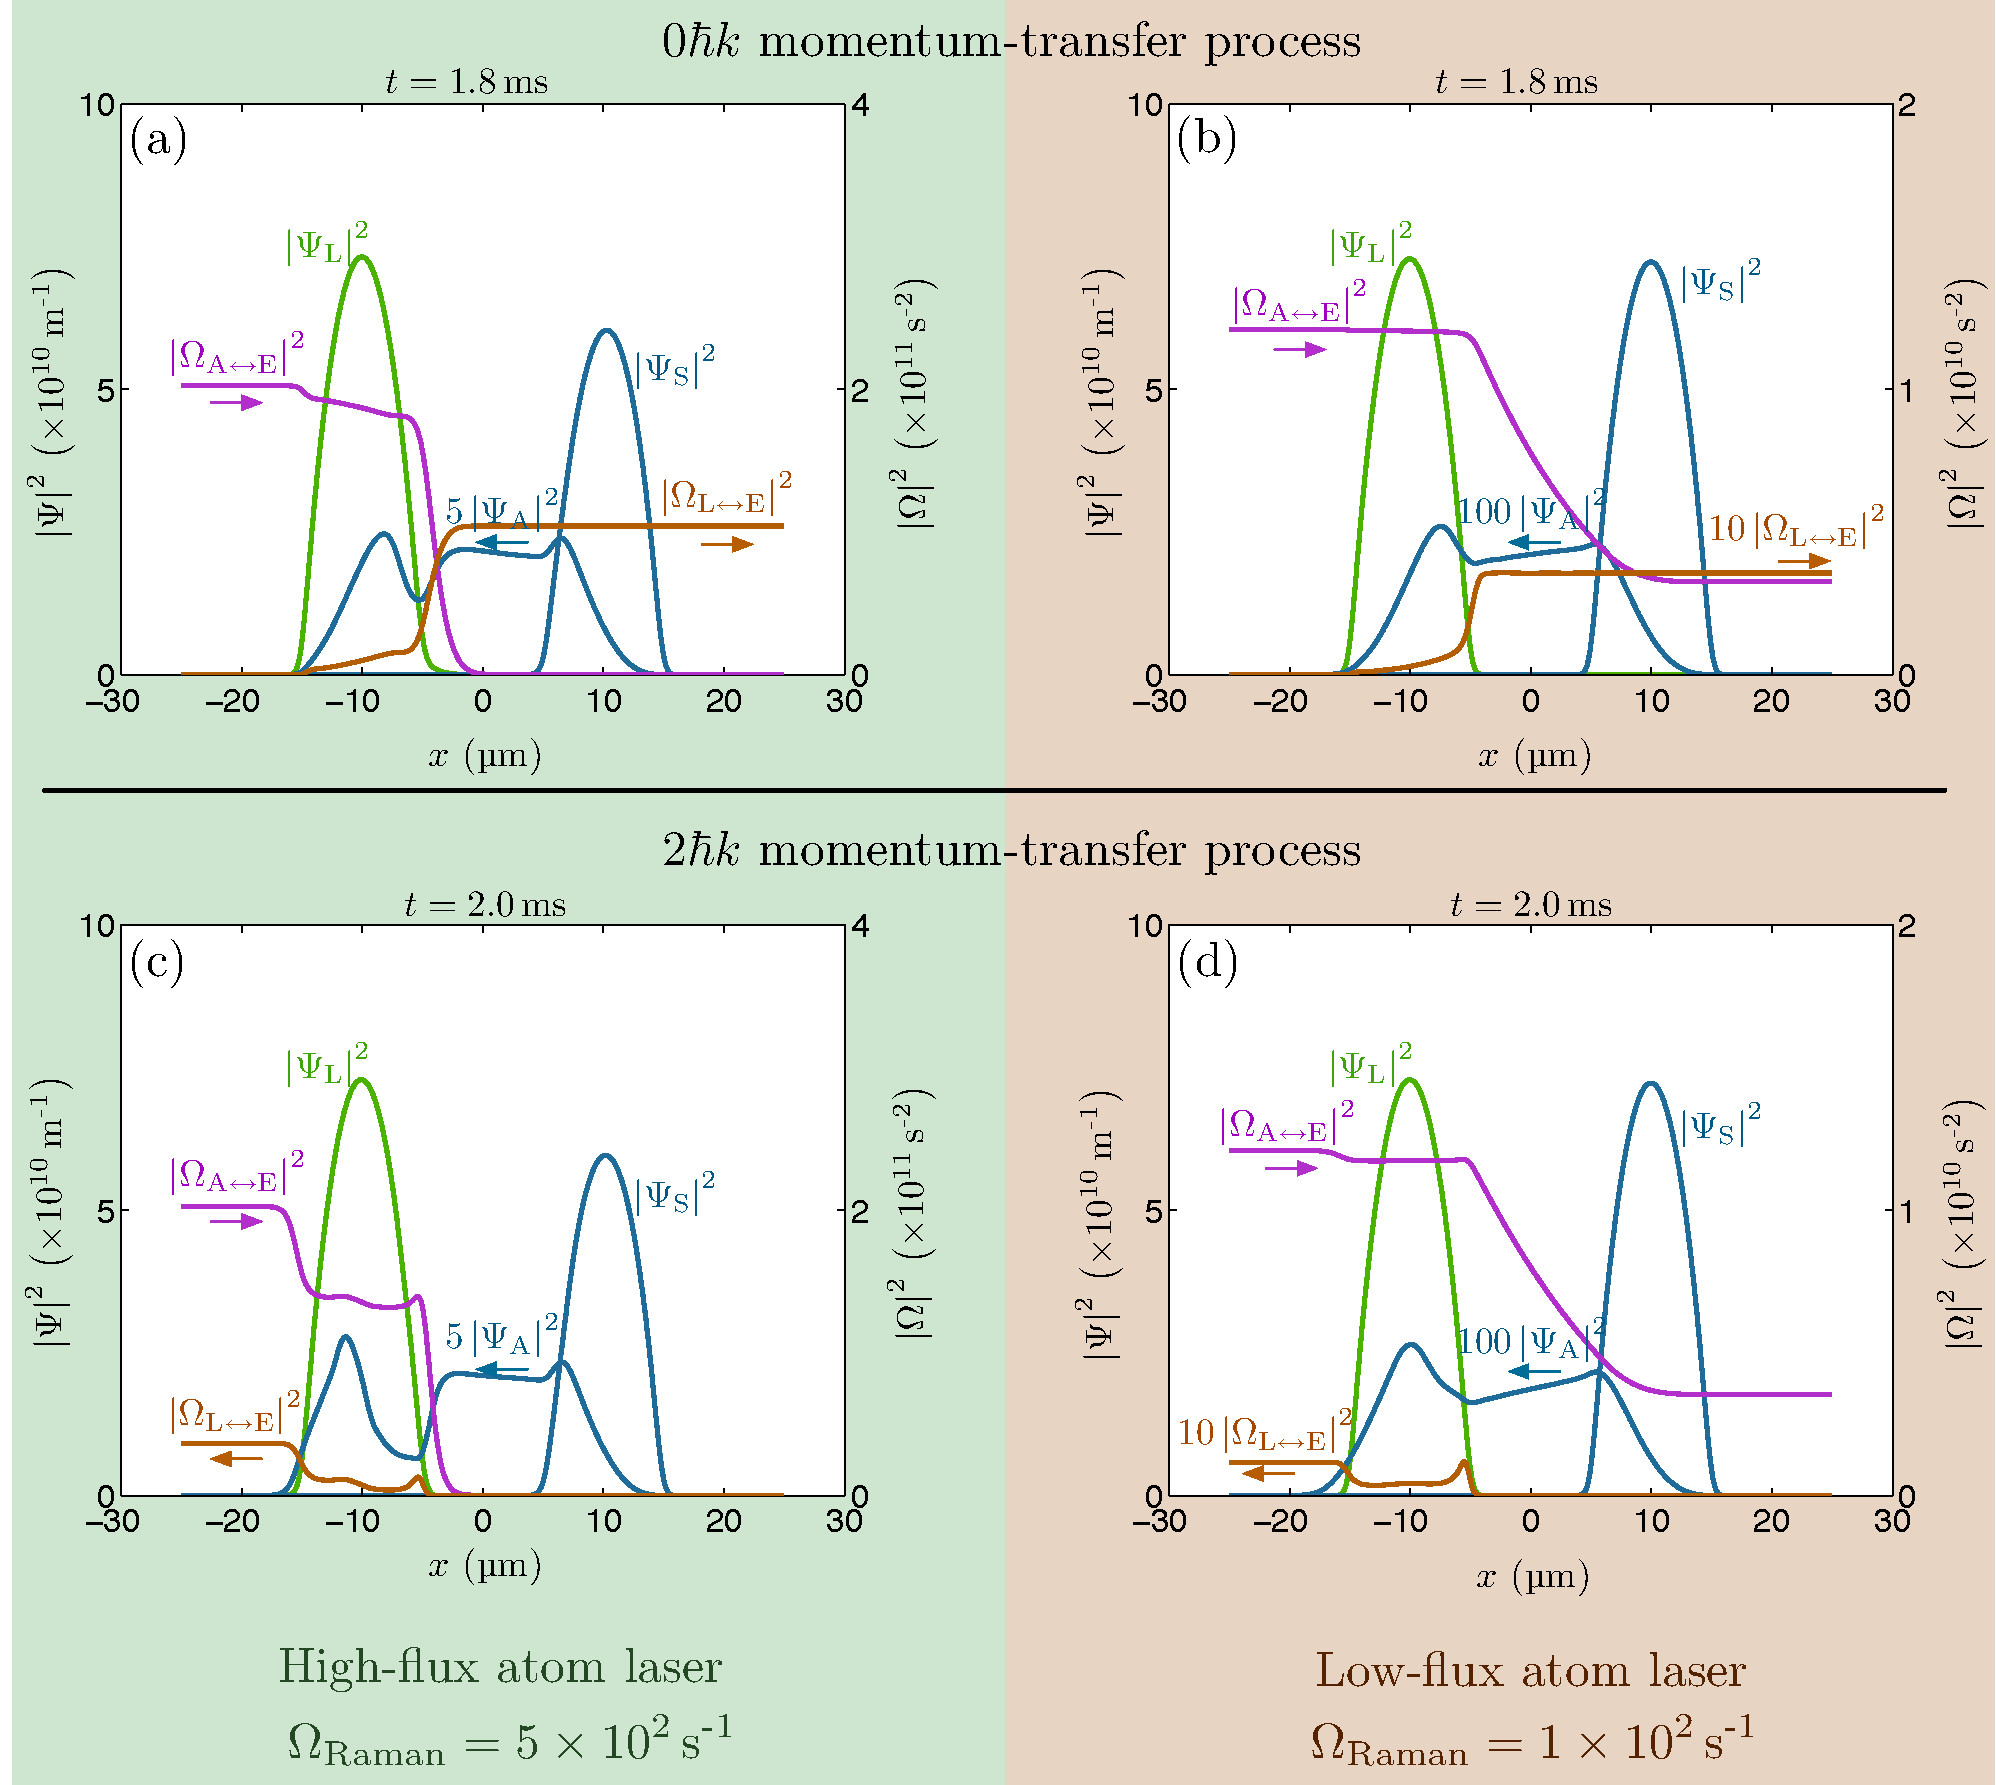
\includegraphics[width=15cm]{TravellingBeamZeroDetuningResults}
    \caption{Simulation results of the simple atom laser model \eqref{OpticalPumping:TravellingBeamEvolution} driven resonantly.  
    The top row is of the $0\hbar k$ momentum-transfer process, which corresponds to the `$+$' sign of \eqref{OpticalPumping:TravellingBeamEvolution:OmegaL}.  
    The bottom row is of the $2\hbar k$ momentum-transfer process, corresponding to the `$-$' sign of \eqref{OpticalPumping:TravellingBeamEvolution:OmegaL}.  
    The figures of the left column consider the limit of a high-flux atom laser ($\Omega_\text{Raman} = 5 \times\unit[10^2]{s\textsuperscript{-1}}$, $\Phi_\text{A} \approx 5 \times \unit[10^7]{s\textsuperscript{-1}}$, $\Omega_{\text{A}\leftrightarrow\text{E}}(-\infty) = 4.5\times \unit[10^5]{s\textsuperscript{-1}}$) in which the transfer efficiency is expected to be greater (see main text).  
    The figures of the right column are in the limit of a lower-flux atom laser ($\Omega_\text{Raman} = 1 \times \unit[10^2]{s\textsuperscript{-1}}$, $\Phi_\text{A} \approx 3\times \unit[10^6]{s\textsuperscript{-1}}$, $\Omega_{\text{A}\leftrightarrow\text{E}}(-\infty) = 1.1\times\unit[10^5]{s\textsuperscript{-1}}$) with a flux similar to that of the continuous pumping experiment.  
    In all simulations the optical pumping laser $\Omega_{\text{A}\leftrightarrow\text{E}}$ is turned on when the atom laser is half-way inside the lasing condensate at $t=\unit[1.6]{ms}$ to approximate equilibrium conditions in a higher-dimensional model (see main text).  The value of $\Omega_{\text{A} \leftrightarrow \text{E}}(-\infty)$ is chosen such that the photon flux balances the atom laser flux.
    Due to the limitations of the 1D nature of this model (see main text), the peak-efficiency of each simulation should be taken to be representative of possible steady-state efficiencies of higher-dimensional models.  The peak-efficiencies of the four simulations are (a) 54\%, (b) 3.5\%, (c) 33\%, (d) 2.7\%.
The different times for the snapshots are chosen to be close to the point of maximum efficiency to best illustrate the transfer process in each case.
    In all simulations the source and lasing condensates are trapped in $\omega = 2 \pi \times \unit[128]{Hz}$ traps, separated by $\unit[20]{\micro m}$ and initially have $N_\text{S} = N_\text{L} = 5 \times \unit[10^5]{atoms}$.
}
    \label{OpticalPumping:TravellingBeamZeroDetuningResults}
\end{figure}

\figureref{OpticalPumping:TravellingBeamZeroDetuningResults} illustrates these conclusions showing some results from the model \eqref{OpticalPumping:TravellingBeamEvolution} for high and low atom laser fluxes.  In particular, the results for higher atom laser fluxes yield higher efficiencies (54\% and 33\% for (a) and (c) respectively) than for lower atom laser fluxes (3.5\% and 2.7\% for (b) and (d) respectively).


\subsubsection{Far detuned limit ($\Delta \gg \Gamma$)}

In the limit of large detuning spontaneous emission should be reduced, however there is still the potential for losses as the atom laser propagates between the source and lasing condensates due to off-resonant interactions with the intense $\Omega_{\text{A} \leftrightarrow \text{E}}$ optical mode.  These losses may be estimated fractionally as
\begin{align}
    r_\text{loss} &= 1 - \exp\left( - \frac{\abs{\Omega_{\text{A} \leftrightarrow \text{E}}}^2}{\Delta^2} \Gamma t \right), \label{OpticalPumping:TravellingBeam:FarDetuned:PropagationLoss}
\end{align}
where $t$ is the time the atom laser takes to propagate from the source to lasing condensates.  Minimising this loss requires
\begin{align}
    \frac{\abs{\Omega_{\text{A} \leftrightarrow \text{E}}}^2}{\Delta^2} \Gamma t \ll 1. \label{OpticalPumping:TravellingBeam:FarDetuned:MinimalPropagationLossRequirement}
\end{align}
Although this is the dominant loss in the system, the remaining fraction of the atom laser may not be fully transferred into the lasing condensate.  The transfer process itself must also be considered to determine the overall behaviour of the pumping mechanism in this limit.

For large detunings spontaneous emission will be suppressed and the photon and atom laser fluxes need not be exactly balanced for a steady-state to be reached, as in the resonant case.  To study the steady-state of the system in the limit that the source and lasing condensate numbers are not changing too quickly, the equations of motion may be simplified by moving into appropriate rotating frames to remove simple phase rotation and neglecting spontaneous emission.  In this limit the source and lasing condensates can be assumed to be constant in time, and the Rabi frequency $\Omega_{\text{A} \leftrightarrow \text{E}}$ will be sufficiently large to be negligibly reduced after propagation through the system and may be assumed to be constant in space.  Our interest is principally in the transfer process itself.  This may be investigated by considering the simplified propagation equations for the atom laser $\Psi_\text{A}$ and the $\Omega_{\text{L} \leftrightarrow \text{E}}$ optical mode as they traverse the lasing condensate in steady state,
\begin{subequations}
    \label{OpticalPumping:TravellingBeam:FarDetuned:SteadyStateEvolution}
    \begin{align}
        \frac{\partial}{\partial x} \Psi_\text{A} &= -i \frac{M}{2 \hbar k} \frac{\Omega_{\text{A}\leftrightarrow\text{E}}^* \Omega_{\text{L} \leftrightarrow \text{E}}^{\phantom{*}}}{\Delta} \Psi_\text{L}, \label{OpticalPumping:TravellingBeam:FarDetuned:SteadyStateEvolution:PsiA}\\
        \frac{\partial}{\partial x} \Omega_{\text{L} \leftrightarrow \text{E}} &= \pm \frac{i}{8} \frac{\Gamma}{\Delta} \frac{\sigma_0}{A_\perp} \Psi_\text{L}^* \Psi_\text{A}^{\phantom{*}} \Omega_{\text{A} \leftrightarrow \text{E}}, \label{OpticalPumping:TravellingBeam:FarDetuned:SteadyStateEvolution:OmegaLE}
    \end{align}
\end{subequations}
where the `$\pm$' sign in \eqref{OpticalPumping:TravellingBeam:FarDetuned:SteadyStateEvolution:OmegaLE} corresponds to propagation of $\Omega_{\text{L} \leftrightarrow \text{E}}$ in the $\pm x$ direction.  These equations can be solved analytically as the phases of $\Psi_\text{L}$ and $\Omega_{\text{A} \leftrightarrow \text{E}}$ may be absorbed into the remaining terms without changing the form of the equations.

The solution for the $0 \hbar k$ momentum-transfer process [the `$+$' sign of \eqref{OpticalPumping:TravellingBeam:FarDetuned:SteadyStateEvolution:OmegaLE}] may be found by applying the boundary conditions
\begin{subequations}
    \begin{align}
        \Psi_\text{A}(x=0) &= \Psi_\text{A}(0), \\
        \Omega_{\text{L} \leftrightarrow \text{E}}(-\infty) &= 0,
    \end{align}
\end{subequations}
where $x=0$ is chosen to be between the source and lasing condensates (see \figureref{OpticalPumping:TravellingBeamZeroDetuningResults}).  The steady-state solution for the atom laser (for $x < 0$) can be shown to be
\begin{align}
    \Psi_\text{A}(x) &= \Psi_\text{A}(0) \frac{e^{w(x) - 2 w(-\infty)} + e^{-w(x)}}{1 + e^{-2 w(x)}},
\end{align}
where $w(x)$ is the dimensionless function
\begin{align}
    w(x) &= \frac{1}{4} \frac{\abs{\Omega_{\text{A} \leftrightarrow \text{E}}}}{\Delta} \sqrt{ \frac{M \Gamma \sigma_0}{\hbar k A_\perp}} \int_{x}^{0} \abs{\Psi_\text{L}}\, dx.
\end{align}
For $w(x) \gg 1$, $\abs{\Psi_\text{A}(x)}^2 \ll \abs{\Psi_\text{A}(0)}^2$ and therefore the atom laser will be almost completely transferred to the lasing condensate.  The efficiency of the transfer process alone is
\begin{align}
    \eta &= 1 - \frac{\abs{\Psi_\text{A}(-\infty)}^2}{\abs{\Psi_\text{A}(0)}^2} = 1-\sech^2\left(\frac{1}{4} \frac{\abs{\Omega_{\text{A} \leftrightarrow \text{E}}}}{\Delta} \sqrt{\frac{M \Gamma \sigma_0}{\hbar k A_\perp}} \int_{-\infty}^{0} \abs{\Psi_\text{L}}\, dx \right) \notag \\
    &= 1-\sech^2\left(\frac{1}{4} \frac{\abs{\Omega_{\text{A} \leftrightarrow \text{E}}}}{\Delta} \sqrt{\frac{M \Gamma \sigma_0}{\hbar k A_\perp}} \int_{-\infty}^{+\infty} \abs{\Psi_\text{L}}\, dx \right),
\end{align}
where the integral has been extended to $+\infty$ as $\Psi_\text{L}(x\geq 0) = 0$ (refer to \figureref{OpticalPumping:TravellingBeamZeroDetuningResults}).

The behaviour of the $2 \hbar k$ momentum-transfer process [the `$-$' sign of \eqref{OpticalPumping:TravellingBeam:FarDetuned:SteadyStateEvolution:OmegaLE}] contrasts strongly with that of the $0 \hbar k$ momentum-transfer process just considered.  For this process the boundary conditions are
\begin{subequations}
    \begin{align}
        \Psi_\text{A}(x=0) &= \Psi_\text{A}(0), \\
        \Omega_{\text{L} \leftrightarrow \text{E}}(+\infty) &= \Omega_{\text{L} \leftrightarrow \text{E}}(0) = 0,
    \end{align}
\end{subequations}
and the solution for the atom laser (for $x < 0$) is
\begin{align}
    \Psi_\text{A}(x) &= \Psi_\text{A}(0) \cos \left(\frac{1}{4} \frac{\abs{\Omega_{\text{A} \leftrightarrow \text{E}}}}{\Delta} \sqrt{\frac{M \Gamma \sigma_0}{\hbar k A_\perp}} \int_{x}^{0} \abs{\Psi_\text{L}} \, dx\right),
\end{align}
In this process, the atoms in the atom laser oscillate between the lasing condensate and the atom laser.  Fundamentally this is because the $\Omega_{\text{L} \leftrightarrow \text{E}}$ photons and the atom laser propagate in the same direction. When an atom is transferred from the atom laser to the lasing condensate a photon in the $\Omega_{\text{L} \leftrightarrow \text{E}}$ mode is created propagating in the same direction.  The photon may later be absorbed by an atom in the lasing condensate transferring the atom back to the atom laser.  In the $0 \hbar k$ momentum-transfer process the $\Omega_{\text{L} \leftrightarrow \text{E}}$ photons and the atom laser propagate in opposite directions.   If by some point the atom laser were completely transferred to the lasing condensate, as the emitted photons propagate in the opposite direction there will be no photons available past this point to transfer atoms from the lasing condensate to the atom laser.  In steady-state, once an atom is transferred from the atom laser to the lasing condensate the emitted photon propagating in the opposite direction will be unavailable to transfer an atom from the lasing mode back to the atom laser.  The difference in the behaviour of the two processes is illustrated in \figureref{OpticalPumping:TravellingBeamFarDetunedResults}.

\begin{figure}
    \centering
    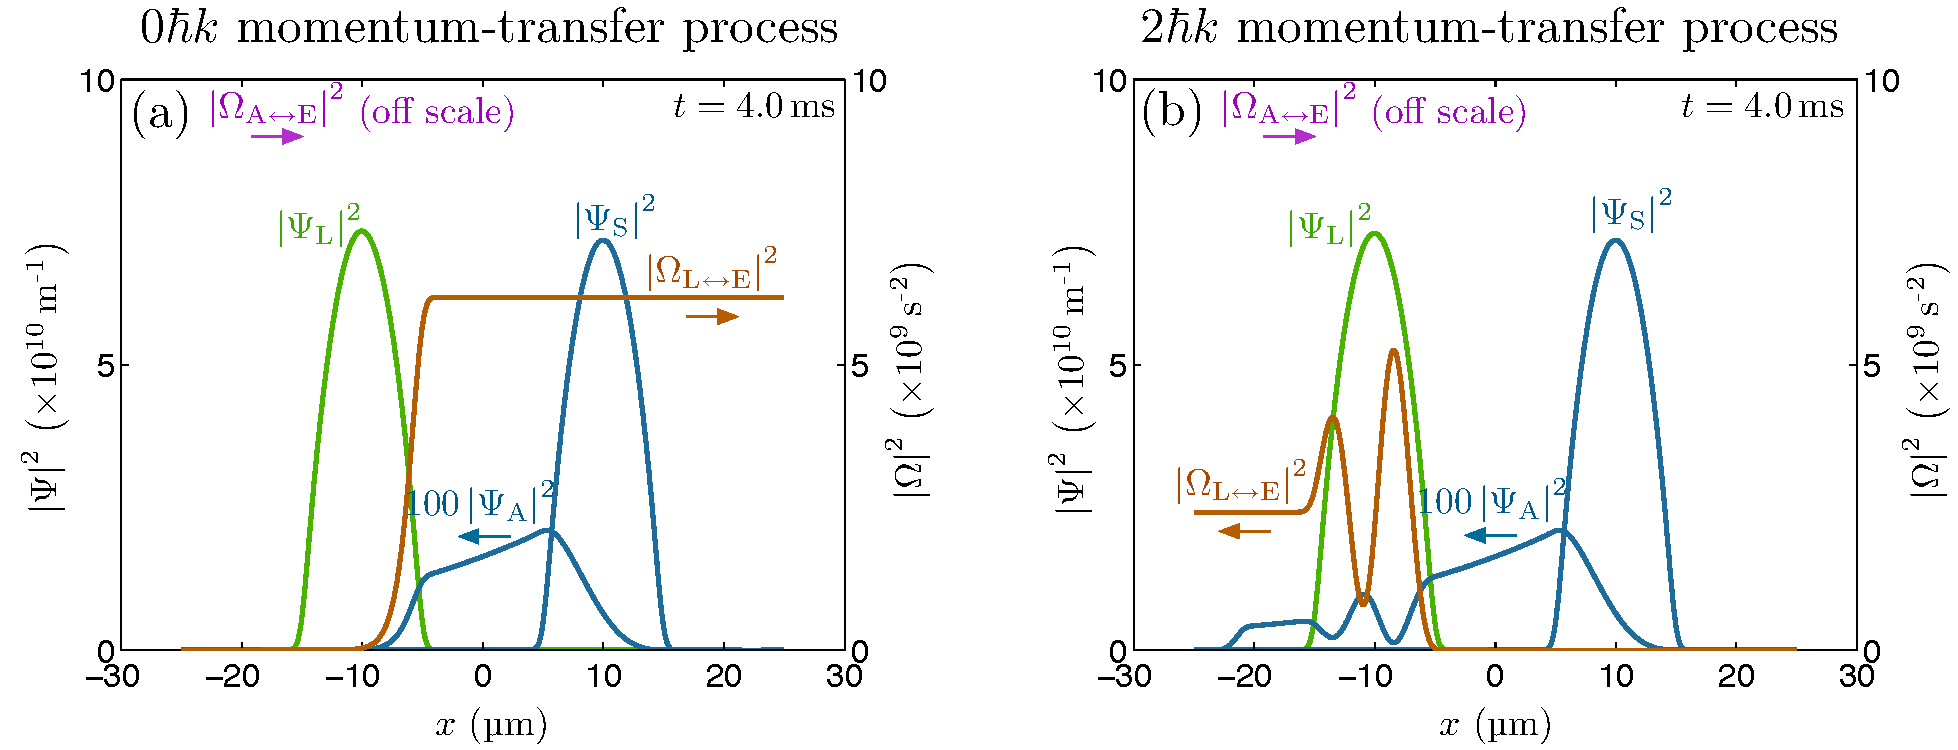
\includegraphics[width=15cm]{TravellingBeamFarDetunedResults}
    \caption{Simulation results of the simple atom laser model \eqref{OpticalPumping:TravellingBeamEvolution} driven by a $\Delta = 10^3 \Gamma = 2 \pi \times \unit[5.9]{GHz}$ detuned optical pumping laser.  Figure (a) is of the $0 \hbar k$ momentum-transfer process, which corresponds to the `$+$' sign of \eqref{OpticalPumping:TravellingBeamEvolution:OmegaL}.  Figure (b) is of the $2 \hbar k$ momentum-transfer process, corresponding to the `$-$' sign of \eqref{OpticalPumping:TravellingBeamEvolution:OmegaL}.  The difference in behaviour of the two processes is quite marked: while in (a) the population transfer is complete, in (b) atoms Rabi flop between the atom laser and the lasing condensate.  These oscillations are damped due to off-resonant spontaneous scattering by the atom laser.  The steady-state efficiencies achieved for these two processes are (a) 48\%, (b) 19\%.  There is an absorbing boundary layer (see \sectionref{BackgroundTheory:AbsorbingBoundaryLayers}) used in both simulations, and this is observed in the sharp decay of the atom laser at the left edge of (b).  In all simulations the optical pumping laser $\Omega_{\text{A} \leftrightarrow \text{E}}$ is approximately constant as it propagates through the system with $\Omega_{\text{A}\leftrightarrow \text{E}}(-\infty) = 1.5 \times \unit[10^8]{s\textsuperscript{-1}}$.  The atom laser is outcoupled from the source condensate with a Rabi frequency $\Omega_\text{Raman} = 1 \times \unit[10^2]{s\textsuperscript{-1}}$.}
    \label{OpticalPumping:TravellingBeamFarDetunedResults}
\end{figure}

Through appropriate choice of detuning and $\Omega_{\text{A} \leftrightarrow \text{E}}$, the $2 \hbar k$ momentum-transfer process can be operated with a high efficiency.  This is however only strictly true for a 1D model.  In higher dimensions the transfer efficiency will reduce because the line integral $\int \abs{\Psi_\text{L}}\, dx$ will vary across the condensate preventing maximum transfer efficiency from being achieved across the entire condensate.  Efficient operation of the detuned $2 \hbar k$ momentum-transfer process in a realistic system is therefore unlikely.  The $0 \hbar k$ momentum-transfer process does not suffer this problem because as the line integral $\int \abs{\Psi_\text{L}}\, dx$ varies across the condensate, as long as the value is sufficiently large the atom laser there will be transferred to the lasing condensate with high efficiency.  Further investigation however is necessary for the $0 \hbar k$ momentum-transfer process.  While it has been shown to be promising in that it displays both Bose-enhancement due to the lasing condensate and robustness to variation in the local condensate density, as mentioned at the start of this section, the $0 \hbar k$ pumping process has been artificially made momentum-resonant.  It would otherwise be impossible for an atom with momentum $2 \hbar k$ to absorb and emit photons with the same momentum to decay into a stationary condensate.  The model of the $0 \hbar k$ momentum-transfer process considered in this section can be considered to approximate the situation in which atoms from the source condensate are outcoupled to form the atom laser before almost immediately undergoing a stimulated transition into the lasing condensate.  This somewhat artificial model was used to permit the $0 \hbar k$ and $2\hbar k$ momentum-transfer processes to be compared on an equal footing where only one of the processes was resonant at a time.  The $0 \hbar k$ momentum-transfer process will be considered further in the next section in which a situation very similar to that of the continuous pumping experiment will be examined.

\subsection{3-level model}
\label{OpticalPumping:3LevelModel}

\begin{figure}
    \centering
    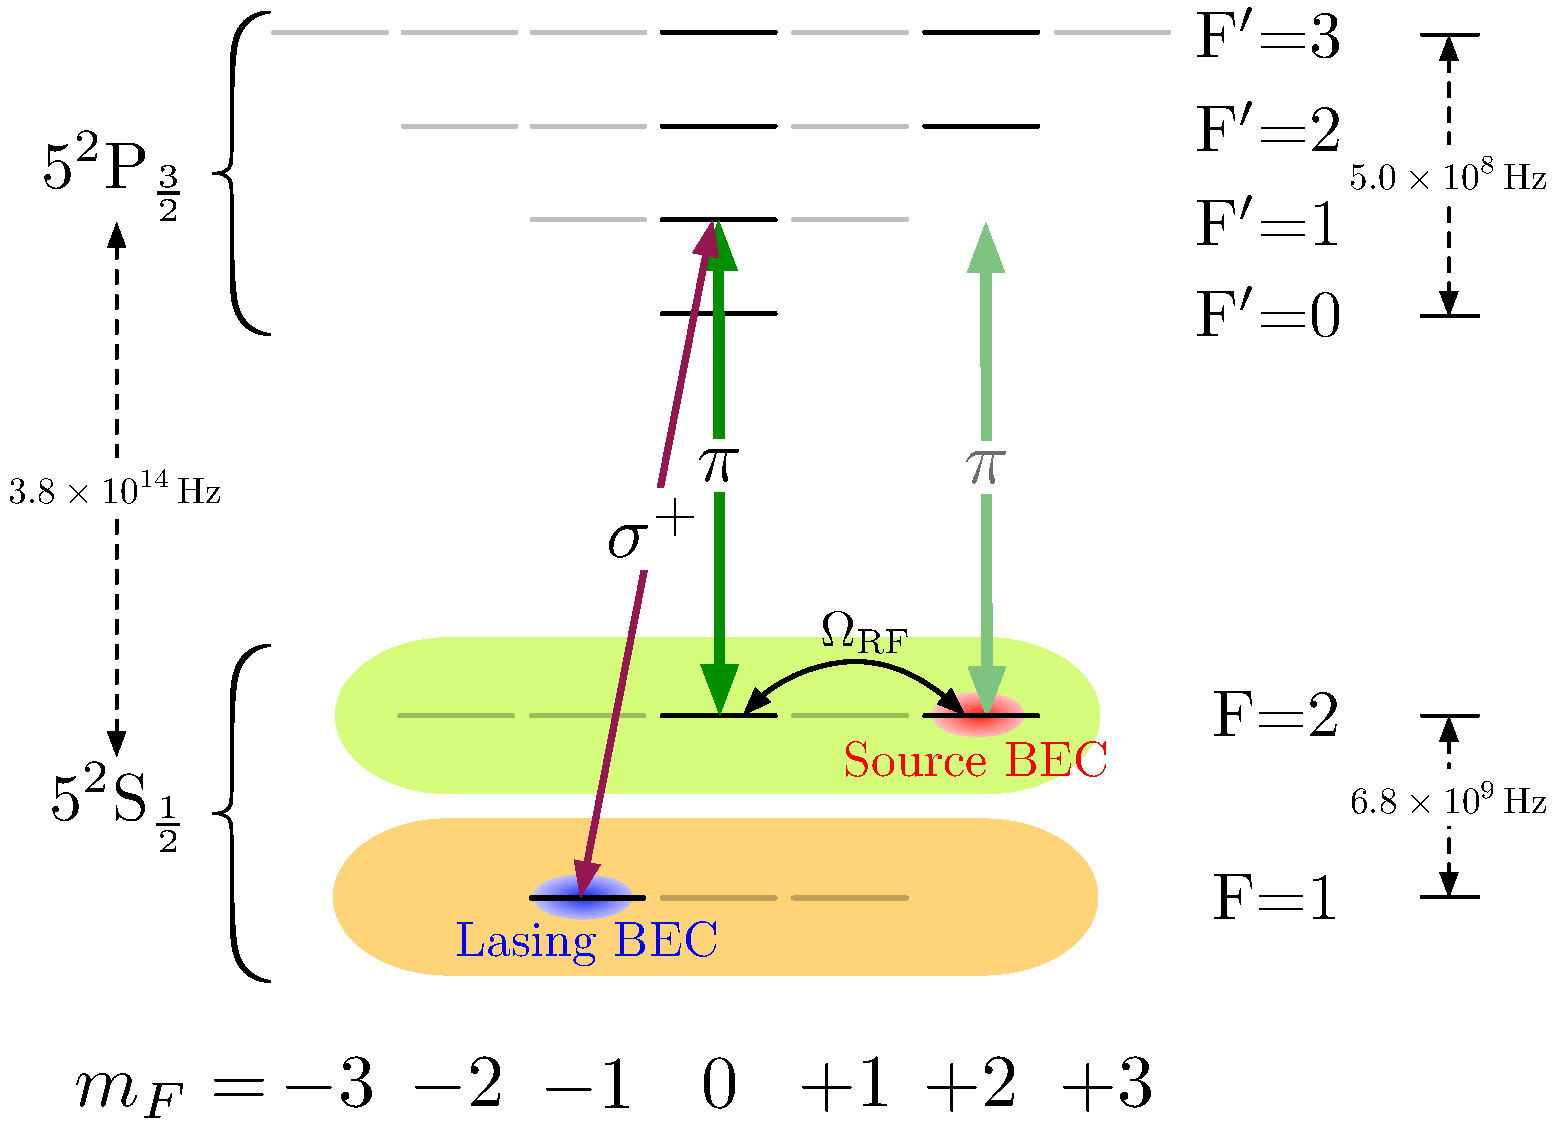
\includegraphics[width=13cm]{3LevelModelLevelDiagram}
    \caption{FIXME: This is not a caption.  Only the levels which have not been greyed out are included in this model.  Of course all the excited levels that haven't been greyed out have still been adiabatically eliminated.  Gravity acts to the left accelerating the initially stationary atom laser from the source condensate towards the lasing condensate.}
    \label{OpticalPumping:3LevelModelLevelDiagram}
\end{figure}

The model of the previous section suggested that the most likely process occurring in the continuous pumping experiment was the $0 \hbar k$ momentum-transfer process.  In this section this prediction will be investigated further by considering a system very similar to that of the continuous pumping experiment.  As it is well known that 5-level atom lasers lead to complicated dynamics \citep{Dugue:2007fk} and our primary focus is on the pumping process itself, we consider a simplification in which the $F=2$ manifold is effectively reduced to a 3-level system by directly coupling the untrapped $\ket{2, 0}$ mode to the source condensate in the $\ket{2, 2}$ state.  In the weak-outcoupling limit considered here the $\ket{2, -2}$ state will be negligibly occupied and it too may be neglected.  A level diagram and schematic of the system under consideration is given in \figureref{OpticalPumping:3LevelModelLevelDiagram}.  

In the present model $\pi$-polarised pumping light is applied from below resonant with the $\ket{F=2, m_F=0} \leftrightarrow \ket{F'=1, m_F=0}$ transition.  Pumping occurs when an atom in the $\ket{F=2, m_F=0}$ state absorbs a $\pi$-polarised photon and is stimulated by the lasing condensate to emit a `$\sigma^+$-polarised' photon.  Due to momentum conservation this `$\sigma^+$-polarised' photon must propagate vertically upwards or downwards (corresponding to the $0\hbar k$ and $2 \hbar k$ momentum-transfer processes, respectively), however pure $\sigma^\pm$-polarised light may only propagate along the direction of the bias field, which is in the horizontal plane in this experiment.  This is because it is the direction of the bias field that defines the atomic polarisations.  The polarisation vector for $\pi$-polarised light is $\unitvec{u}_\pi = \unitvec{z}$ where $\unitvec{z}$ is the unit vector in the direction of the bias field (also the weak trapping axis).  Pure $\pi$-polarised light may therefore propagate vertically (i.e.\ in the $\pm \unitvec{y}$ direction).  The polarisation vectors for $\sigma^\pm$-polarised light are $\unitvec{u}_{\sigma^\pm} = \frac{1}{\sqrt{2}} (\unitvec{x} \pm i \unitvec{y})$.  As neither of these polarisation vectors are orthogonal to $\unitvec{y}$, they cannot propagate in this direction.  The polarisation that propagates vertically that the $\ket{F=1, m_F=-1} \leftrightarrow \ket{F'=1, m_F=0}$ transition is coupled to is the polarisation orthogonal to that of the $\pi$-polarised photons travelling in this direction, i.e.\ they will be polarised along the $\unitvec{x}$ direction.  We label this polarisation $\pislash$ with $\unitvec{u}_\pislash = \unitvec{x}$.  When an atom makes a transition from $\ket{F'=1, m_F=0}$ to $\ket{F=1, m_F=-1}$ stimulated by the lasing condensate the emitted photon therefore is $\pislash$-polarised, a superposition of the $\sigma^+$ and $\sigma^-$ polarisations.

The equations of motion for this system are derived directly from the general multimode model of \eqref{OpticalPumping:GeneralMultimodeModel}.  The evolution of the atomic fields is given by
\begin{subequations}
    \begin{align}
        \begin{split}
            i \hbar \frac{\partial}{\partial t} \Psi_{2,2} &= \left[- \frac{\hbar^2}{2 M} \frac{\partial^2}{\partial y^2} + 2 V_\text{trap}(y) + M g y + U_\text{1D}\left(\abs{\Psi_{2, 2}}^2 + \abs{\Psi_{2, 0}}^2 + \abs{\Psi_{1, -1}}^2\right)\right] \Psi_{2, 2} \\
            &\relphantom{=} + \hbar \Omega_\text{RF}^* \Psi_{2, 0} -i \hbar\, Q(2,2 \xrightarrow{\pi,\pi} 2, 2) \abs{E_\pi}^2 \Psi_{2, 2},
        \end{split}\\
        \begin{split}
            i \hbar \frac{\partial}{\partial t} \Psi_{2, 0} &= \left[ - \frac{\hbar^2}{2M} \frac{\partial^2}{\partial y^2} + 2 \hbar \Delta_\text{RF} + M g y + U_\text{1D}\left(\abs{\Psi_{2, 2}}^2 + \abs{\Psi_{2, 0}}^2 + \abs{\Psi_{1, -1}}^2\right)\right] \Psi_{2, 0} \\
            &\relphantom{=} + \hbar \Omega_\text{RF} \Psi_{2, 2}  - i \hbar \,Q({2, 0 \xrightarrow{\pi,\pi} 2, 0}) \abs{E_\pi}^2 \Psi_{2, 0} - i \hbar \,Q(2, 0 \xrightarrow{\pi,\pislash} 1, -1) E_\pi^* E_{\pislash}^{\phantom{*}} \Psi_{1, -1},
        \end{split}\\
        \begin{split}
            i \hbar \frac{\partial}{\partial t} \Psi_{1, -1} &= \left[ - \frac{\hbar^2}{2 M} \frac{\partial^2}{\partial y^2} + V_{\text{trap}}(y) + M g y + U_\text{1D} \left( \abs{\Psi_{2, 2}}^2 + \abs{\Psi_{2, 0}}^2 + \abs{\Psi_{1, -1}}^2\right)  \right] \Psi_{1, -1}\\
            &\relphantom{=} - i \hbar \,Q(1, -1 \xrightarrow{\pislash,\pislash} 1, -1) \abs{E_{\pislash}}^2 \Psi_{1, -1} - i \hbar \,Q(1, -1 \xrightarrow{\pislash,\pi} 2, 0) E_{\pislash}^* E_\pi^{\phantom{*}}\Psi_{2, 0},
        \end{split}
    \end{align}
\end{subequations}
where $\Psi_{F,f}$ is the wavefunction for the atomic state $\ket{F, f}$; $E_\alpha$ is the electric field for polarisation $\alpha$; $V_\text{trap}(y) = \frac{1}{2} M \omega_y^2 y^2$; $\Delta_\text{RF}$ is the detuning of the rf outcoupling; $g$ is the acceleration due to gravity and the two-photon coupling constants between atomic state $\ket{F, f}$ and $\ket{G, g}$ are
\begin{align}
    Q(F, f \xrightarrow{\alpha, \beta} G, g) &= \sum_{F',f'}\frac{1}{\frac{1}{2}\Gamma + i \Delta_{F',f'}} \frac{(\vect{d}_{F, f; F', f'} \cdot \unitvec{u}_\alpha^*)}{\hbar} \frac{(\vect{d}_{G, g; F', f'}^* \cdot \unitvec{u}_\beta^{\phantom{*}})}{\hbar};
\end{align}
where the sum over $\{F', f'\}$ extends over all excited levels $\ket{F', f'}$ coupled to both $\ket{F, f}$ and $\ket{G, g}$; and $\Delta_{F', f'}$ is the detuning of the excited state $\ket{F', f'}$ relative to the optical modes.

To consider both the $0 \hbar k$ and $2 \hbar k$ momentum-transfer processes, we split the electric fields for each polarisation into both upward and downward propagating components,
\begin{align}
    E_{\alpha}(y) &= E_{\alpha, \text{up}}(y) + E_{\alpha, \text{down}}(y).
\end{align}
These electric field components evolve as
\begin{subequations}
    \begin{align}
        \begin{split}
            \frac{\partial}{\partial y}E_{\pi, \text{up}} &= i k E_{\pi, \text{up}} - \frac{\hbar k}{2 \varepsilon_0 A_\perp} Q({2, 0 \xrightarrow{\pi,\pislash} 1, -1}) \Psi_{2, 0}^* \Psi_{1, -1} E_{\pislash}\\
            &\relphantom{=} - \frac{\hbar k}{2 \varepsilon_0 A_\perp} \left[Q({2, 2 \xrightarrow{\pi,\pi} 2, 2}) \abs{\Psi_{2, 2}}^2  + Q({2, 0 \xrightarrow{\pi,\pi} 2, 0}) \abs{\Psi_{2, 0}}^2 \right] E_{\pi, \text{up}},
        \end{split}\\
        \begin{split}
            -\frac{\partial}{\partial y}E_{\pi, \text{down}} &= i k E_{\pi, \text{down}} - \frac{\hbar k}{2 \varepsilon_0 A_\perp} Q({2, 0 \xrightarrow{\pi,\pislash} 1, -1}) \Psi_{2, 0}^* \Psi_{1, -1} E_{\pislash}\\
            &\relphantom{=} - \frac{\hbar k}{2 \varepsilon_0 A_\perp} \left[Q({2, 2 \xrightarrow{\pi,\pi} 2, 2}) \abs{\Psi_{2, 2}}^2  + Q({2, 0 \xrightarrow{\pi,\pi} 2, 0}) \abs{\Psi_{2, 0}}^2 \right] E_{\pi, \text{down}},
        \end{split}\\
        \begin{split}
            \frac{\partial}{\partial y}E_{\pislash, \text{up}} &= i k E_{\pislash, \text{up}} - \frac{\hbar k}{2 \varepsilon_0 A_\perp} Q({2, 0 \xrightarrow{\pi,\pislash} 1, -1}) \Psi_{1, -1}^* \Psi_{2, 0} E_{\pi} \\
            &\relphantom{=} - \frac{\hbar k}{2 \varepsilon_0 A_\perp} Q({1, -1 \xrightarrow{\pislash,\pislash} 1, -1}) \abs{\Psi_{1, -1}}^2 E_{\pislash, \text{up}} ,
        \end{split}\\
        \begin{split}
            -\frac{\partial}{\partial y}E_{\pislash, \text{down}} &= i k E_{\pislash, \text{down}} - \frac{\hbar k}{2 \varepsilon_0 A_\perp} Q({2, 0 \xrightarrow{\pi,\pislash} 1, -1}) \Psi_{1, -1}^* \Psi_{2, 0} E_{\pi} \\
            &\relphantom{=} - \frac{\hbar k}{2 \varepsilon_0 A_\perp} Q({1, -1 \xrightarrow{\pislash,\pislash} 1, -1}) \abs{\Psi_{1, -1}}^2 E_{\pislash, \text{down}}.
        \end{split}
\end{align}
\end{subequations}

The dipole moments for the various transitions can be written as multiples of the reduced dipole matrix element for the $\text{D}_2$ transition by the Wigner-Eckart theorem \citep{Eckart:1930,Brink:1962}
\begin{align}
    \vect{d}_{F,f;F',f'} &= c_{F,f;F',f'} d_\text{reduced} \unitvec{u}_\alpha,
\end{align}
where $\alpha\in \{\pi,\sigma^\pm\}$ is the polarisation corresponding to the $\ket{F, f} \leftrightarrow \ket{F', f'}$ transition, $d_\text{reduced} = \left<J=\frac{1}{2} \middle\| e r \middle\| J'=\frac{3}{2}\right> = 3.6 \times \unit[10^{-29}]{C.m}$ is the reduced dipole matrix element for the $\text{D}_2$ transition in $^{87}\text{Rb}$, and $c_{F, f; F', f'}$ is a real constant given by \citep{Steck:2009}
\begin{align}
    \label{OpticalPumping:DipoleMomentCoefficient}
    c_{F,f;F',f'} &= (-1)^{J +I + f} \sqrt{(2 F + 1)(2F' + 1)(2J + 1)}
    \begin{Bmatrix} 
        J & J' & 1 \\
        F' & F & I 
    \end{Bmatrix}
    \begin{pmatrix}
        F' & 1 & F\\
        f' & f - f' & -f
    \end{pmatrix},
\end{align}
where the array in braces is a Wigner $6j$ symbol, and the array in parentheses is a Wigner $3j$ symbol.  For the $5^2\text{S}_{\frac{1}{2}} \rightarrow 5^2\text{P}_{\frac{3}{2}}$ transition of $^{87}\text{Rb}$, the remaining quantum numbers in \eqref{OpticalPumping:DipoleMomentCoefficient} are $I = \frac{3}{2}$, $J = \frac{1}{2}$, and $J' = \frac{3}{2}$.  Values for $c_{F, f; F', f'}$ may be found in standard tables \citep{Steck:2009}.  The two most important dipole moments are
\begin{align}
    \vect{d}_{1, -1; 1', 0'} &=  \sqrt{\frac{5}{24}} d_\text{reduced} \unitvec{u}_{\sigma^+},\\
    \vect{d}_{2, 0; 1', 0'} &= \sqrt{\frac{1}{30}} d_\text{reduced} \unitvec{u}_\pi.
\end{align}

The usual technique for reducing a 3D model to a 1D model cannot be applied to the present system without ambiguity.  The usual method aims to derive an effective 1D interaction strength $U_\text{1D}$ from the 3D interaction strength $U_\text{3D}$ by dividing it by a representative transverse area $A_\perp$, i.e.\ $U_\text{1D} = U_\text{3D}/A_\perp$.  This transverse area is typically chosen such that the chemical potentials of the two models are equal (and hence the corresponding Thomas-Fermi radii are equal).  In the present model there are two possible transverse areas to choose corresponding to each of the two condensates.  Although the transverse areas depend on the condensate number, the primary difference is due to the different trapping frequencies: those for the $\ket{2, 2}$ atoms are $\sqrt{2}$ times larger than those for the $\ket{1, -1}$ atoms.  In resolving this problem we would like to preserve the Thomas-Fermi radii of both condensates because, as discussed at the end of \sectionref{OpticalPumping:ContinuousExperiment}, the slight overlap of the two condensates may be crucially important for the operation of the pumping mechanism.

To make the dimension reduction, we choose the transverse area corresponding to the source condensate (the $\ket{2, 2}$ state) $A_\perp = 2.8 \times\unit[10^{-10}]{m\textsuperscript{2}}$, as this should be representative for both the source condensate and the atom laser in the $\ket{2, 0}$ state.  To make the Thomas-Fermi radius of the lasing condensate (the $\ket{1, -1}$ state) match that of a 3D model, we decrease the number of atoms in this state.  This reduces the effective number of atoms in the lasing condensate from $N_\text{lasing} = 5.0\times 10^5$ to $N_\text{lasing}^\text{(eff)} = 4.3\times 10^5$.  This reduction in the condensate number causes the density of the lasing condensate to be lower than it otherwise would be in the 1D model; in a 3D model the density would be lower because of the larger transverse area.

\parasep

With the model itself explained, we may now use it to investigate the hypothesis that it is the $0 \hbar k$ momentum-transfer process that occurs in the continuous pumping experiment.  To this end, a parameter scan of the model was performed to find the maximum transfer efficiency as a function of outcoupling detuning for a fixed atom laser flux $\Phi = \unit[1\times 10^7]{s\textsuperscript{-1}}$ for $\unit[3]{ms}$ of outcoupling.  For each outcoupling detuning $\Delta_\text{RF}$, a parameter scan was performed as a function of the intensity of the applied optical pumping light (as determined by $E_{\pi, \text{up}}(-\infty)$) to determine the optimum pumping efficiency.  If the pumping light intensity is too low the transfer process will proceed slowly, while if the pumping light is too intense spontaneous losses from the atom laser and the source condensate will exceed the atom number transferred to the lasing condensate.  The optimum pumping efficiency (ratio of the number of atoms transferred to the lasing condensate divided by the number of atoms lost from the source condensate) is plotted as a function of the outcoupling detuning in \figureref{OpticalPumping:3LevelModelEfficiency}.

\begin{figure}
    \centering
    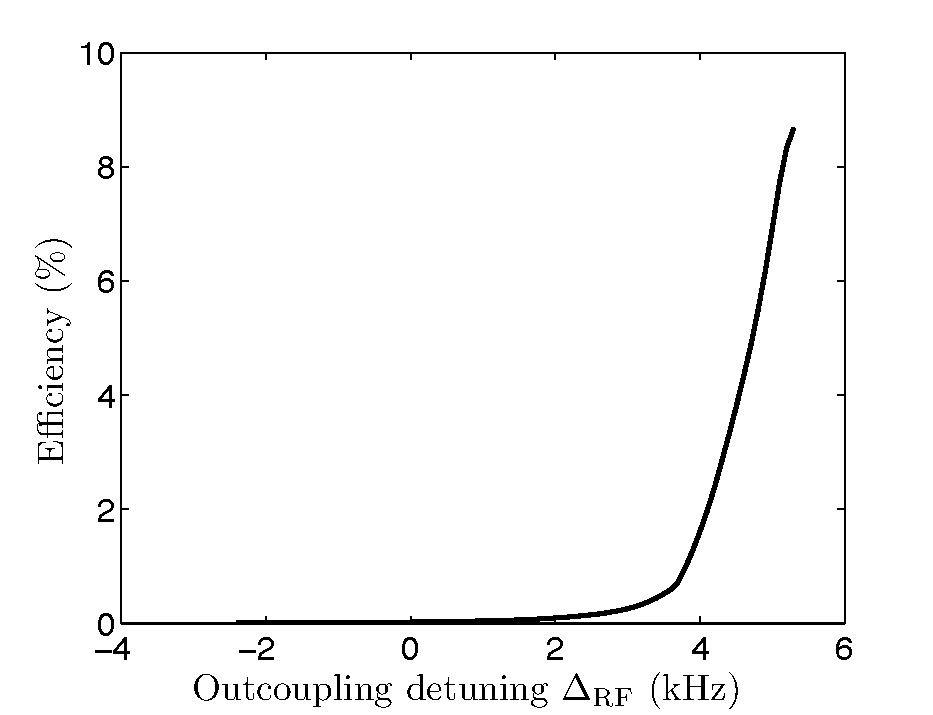
\includegraphics[width=8cm]{3LevelModelEfficiency}
    \caption{FIXME: This is not a caption. $\unit[3]{ms}$ of outcoupling, a flux of $\Phi = 1\times \unit[10^7]{s\textsuperscript{-1}}$.  $\Delta_\text{RF} =0$ corresponds to the energy resonance of the outcoupling process being in the centre of the condensate.}
    \label{OpticalPumping:3LevelModelEfficiency}
\end{figure}

The plot of pumping efficiency \figureref{OpticalPumping:3LevelModelEfficiency} shows a clear increase in efficiency at large detunings where the $0 \hbar k$ momentum-transfer process is expected to occur.  It is interesting to note that there isn't a local maximum near $\Delta_\text{RF} = 0$ where the $2 \hbar k$ momentum-transfer process would be expected to occur.  Examining the dynamics of a simulation in this parameter regime illuminates the reason.  \figureref{OpticalPumping:3LevelParameterScanSnapshots}(a) illustrates a snapshot of a simulation of the system with $\Delta_\text{RF}= 0$.  What is occurring is that as the atom laser falls, it first comes into momentum-resonance with the lasing condensate (via the $2 \hbar k$ momentum-transfer process) towards the upper edge of the lasing condensate, however it goes out of momentum-resonance within the lower half of the lasing condensate as the atom laser continues to accelerate under gravity.  As this occurs the system attempts to follow the dark state by compensating for the reduction in the density of the atom laser that is momentum-resonant with the lasing condensate by transferring atoms from the lasing condensate back to the atom laser.  As this process requires photons in the $E_{\pislash, \text{down}}$ mode to occur, the number of atoms transferred back to the atom laser is limited by the number of atoms transferred from the atom laser to the lasing condensate at the upper edge of the lasing condensate.  As a result there is a negligible net transfer of atoms to the lasing condensate.  Counter-intuitively, the only way to $2 \hbar k$ momentum-transfer process can operate is not by having the atom laser momentum-resonant at the \emph{centre} of the lasing condensate where the condensate density is a maximum, but instead to have the atom laser momentum-resonant towards the lower edge of the lasing condensate.  This way the lasing condensate density will reduce before the atom laser is no longer momentum-resonant with the lasing condensate.  As the system follows the dark state it will attempt to compensate for the loss of density of the lasing condensate by transferring atoms from the atom laser into the lasing condensate.  This therefore requires outcoupling from the lower part of the source condensate, the same parameter regime in which the $0 \hbar k$ momentum-transfer process is expected to operate.  However for the reasons discussed in \sectionref{OpticalPumping:SimpleModels:AtomLaserModel}, the $0 \hbar k$ momentum-transfer process will be expected to dominate as it will suffer significantly less spontaneous loss.

\begin{figure}
    \centering
    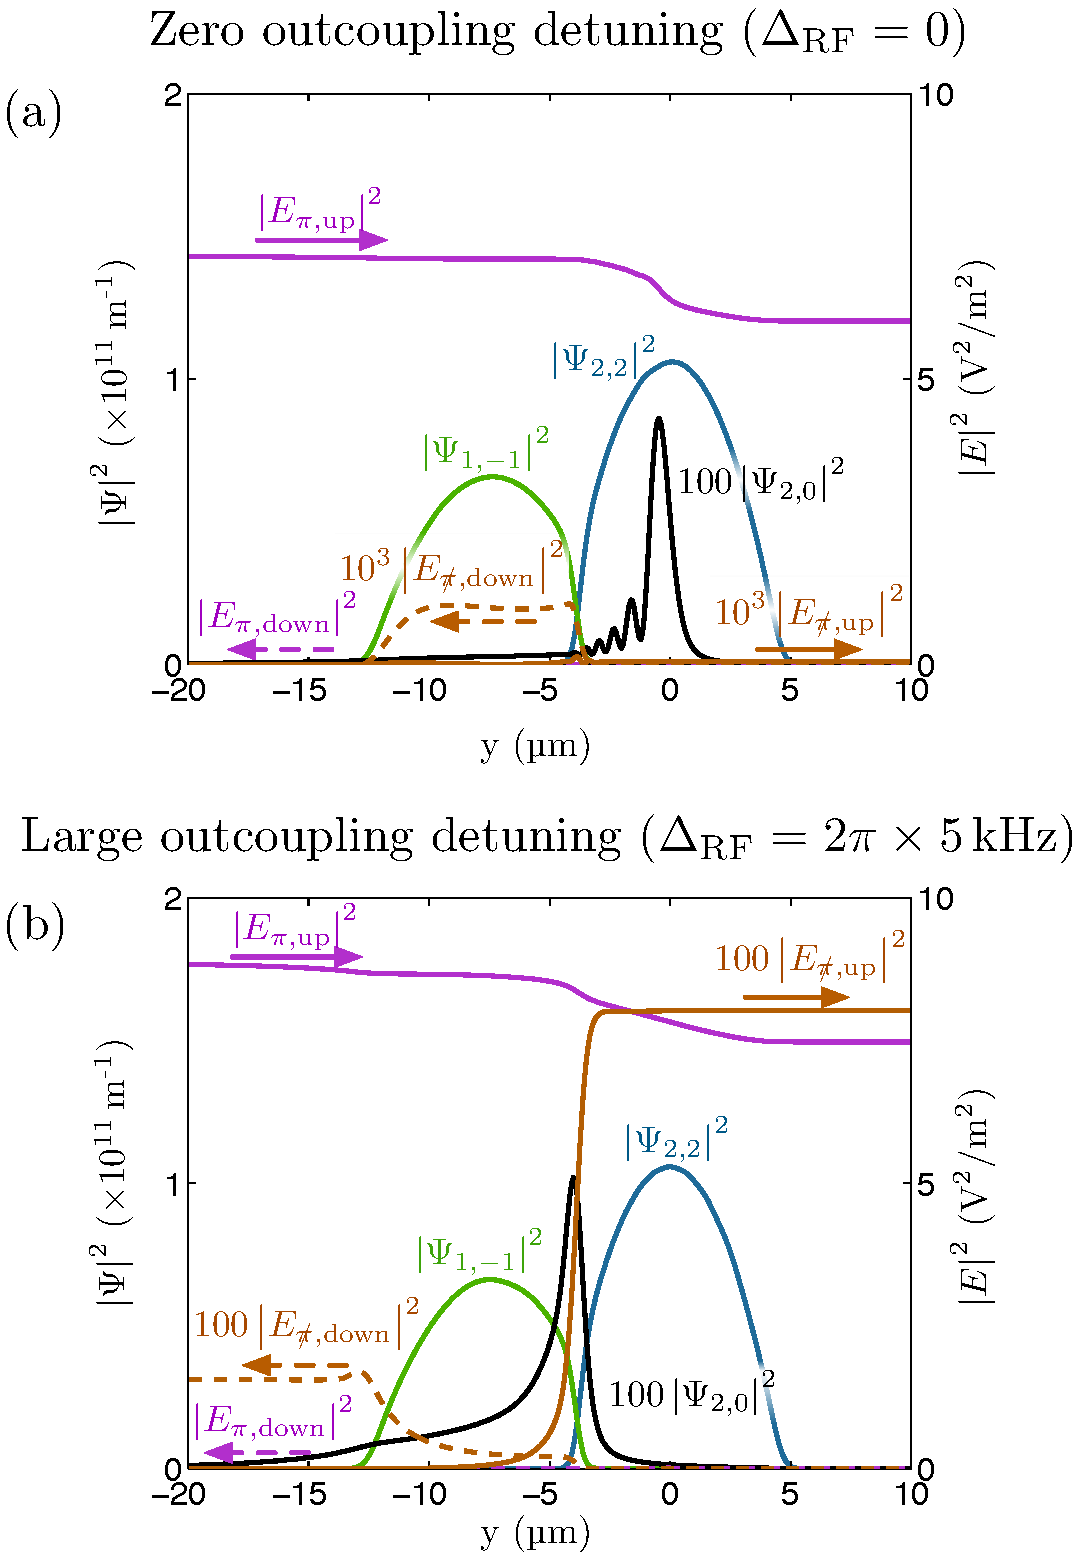
\includegraphics[width=10cm]{3LevelParameterScanSnapshots}
    \caption{FIXME: This is not a caption. (a) $E_{\pi,\text{up}}(-\infty) = \unit[2.6741509905]{V/m}$, $\Omega_\text{RF} = \unit[263.66]{s\textsuperscript{-1}}$, $\Delta_\text{RF} = 0.0$. (b) $E_{\pi, \text{up}}(-\infty) = \unit[2.97398865843]{V/m}$, $\Omega_\text{RF} = \unit[702.53]{s\textsuperscript{-1}}$, $\Delta_\text{RF} = 2 \pi \times \unit[5]{kHz}$.  It is readily observed that the outcoupling position of the atom laser $\Psi_{2, 0}$ is shifted significantly approximately $\unit[5]{\micro m}$ down into the region of overlap between the two condensates. All snapshots are taken at $t = \unit[3]{ms}$.}
    \label{OpticalPumping:3LevelParameterScanSnapshots}
\end{figure}

\figureref{OpticalPumping:3LevelParameterScanSnapshots}(b) illustrates a snapshot of a simulation of the system for $\Delta_\text{RF} = 2\pi \times \unit[5]{kHz}$, a parameter regime in which the $0 \hbar k$ momentum-transfer process is expected to be significant.  The operation of the $0 \hbar k$ momentum-transfer process is signalled by the population of the $E_{\pislash, \text{up}}$ mode after propagation through the system.  Additionally, the occupation of the $E_{\pislash, \text{down}}$ mode indicates that the $2 \hbar k$ momentum-transfer process is also occurring, although to a lesser extent.  


Over the simulated time of $t = \unit[3]{ms}$ the pumping efficiency for the simulation illustrated in \figureref{OpticalPumping:3LevelParameterScanSnapshots}(b) is 5.9\%.  While $\unit[3]{ms}$ of outcoupling and pumping cannot fully represent the behaviour of the system for the entire $\unit[100]{ms}$ to $\unit[200]{ms}$ over which the pumping occurred in the experiment, it does give a general indication of the behaviour of the system.  Do to the prohibitive computing time that would be required to do a full parameter scan for a pumping time of 100's of milliseconds, a numerical optimisation procedure was instead used to determine the optimum efficiency achievable from the experiment over $\unit[150]{ms}$.  \footnote{FIXME: Something is missing here.  Is it necessary to discuss the things that were necessary to consider in the numerical optimisation procedure?  Things like maximising transfer into the condensate mode?}Over these longer timescales it was observed that the $2 \hbar k$ momentum-transfer process contributed relatively little to the total population transfer.  This is because the lower edge of the lasing condensate moved downwards as it increased in size while the position at which the atom laser was momentum-resonant via the $2 \hbar k$ momentum-transfer process remained stationary.  FIXME: Integrate results: efficiency 6.8\%, detuning: $\Delta_\text{RF} = 2\pi \times \unit[4.6]{kHz}$, $E_{\pi, \text{up}}(-\infty) = \unit[4.8975]{V/m}$, $\Omega_\text{RF} = 1.9413\times \unit[10^3]{s\textsuperscript{-1}}$.


\subsubsection{Comparison with experiment}

The preceding modelling strongly indicates that the pumping process occurring in the continuous pumping experiment was the $0 \hbar k$ momentum-transfer process.  If true, this significantly impacts the potential applicability of the pumping mechanism of that experiment to a future continuously pumped atom laser.  It was intended that the continuous pumping experiment could be extended to the production of a continuously pumped atom laser by replacing the source condensate once it becomes depleted with an independently produced condensate, which becomes the new source condensate.  As the pumping mechanism is independent of the relative phase of the source and lasing condensates, this would enable the operation of a continuously pumped atom laser, the atomic analogue to the continuous optical laser.  However if the lasing condensate must spatially overlap with the source condensate for the pumping mechanism to operate (as is the case for the $0 \hbar k$ momentum-transfer process), the source condensate cannot be replaced without necessarily disturbing the lasing condensate.  This unavoidable excitation would disrupt the narrow linewidth properties that are desired of a continuously pumped atom laser.

The conclusions drawn from the preceding model are however only valid to the extent that the model is representative of the system under study.  There remain some details of the experiment that have not been fully considered.

The first is that the outcoupling process from the source condensate has been simplified to remove the $\ket{F=2, m_F = 1}$ atoms [see \figureref{OpticalPumping:3LevelModelLevelDiagram}(a)].  In the continuous pumping experiment, the applied RF radiation coupled the entire $F=2$ manifold, with each level coupled to the next.  While the anti-trapped levels $\ket{F=2, m_F=-1}$ and $\ket{F=2, m_F=-2}$ are unlikely to have played a significant role as the RF outcoupling was weak, the $\ket{F=2, m_F=1}$ level could potentially have an impact as it is via this level that atoms are outcoupled into the untrapped $\ket{F=2, m_F=0}$ state, the only state that can undergo stimulated transitions into the lasing condensate (via the $\ket{F'=1, m_F=0}$ state).  The inclusion of the $\ket{F=2, m_F=1}$ level is unlikely to affect the conclusion that it is the $0 \hbar k$ momentum-transfer process that is occurring in the experiment as the $\ket{F=2, m_F=1}$ level is resonant with the $\pi$-polarised pumping light (see \figureref{OpticalPumping:LevelDiagram}), leading to the same overall losses for the $2 \hbar k$ momentum-transfer process independent of what proportion of their falling time the atoms spend in the $\ket{F=2, m_F=1}$ or $\ket{F=2, m_F=0}$ states.  It is infeasible at present to further investigate this issue numerically as the system would need to be simulated in at least two dimensions when including the $\ket{F=2, m_F=1}$ level for reasons discussed in \sectionref{OpticalPumping:5LevelModel}.

The second detail of the experiment that is not fully understood is the difference between the optimum efficiency determined theoretically 6.8\% and that observed in the experiment $(35\pm 10)\%$.  It is unusual for theory to predict a lower efficiency than is observed in the experiment.  Usually theory predicts a larger effect or efficiency than is observed experimentally (an obvious exception being initial attempts at doppler cooling) due to experiment differing from the idealised scenario considered theoretically.  It seems unlikely that the difference in this instance could be due to the absence of the $\ket{F=2, m_F=1}$ level from the present model as the spatial dynamics of the present model should be simpler than that of a full model, leading to a higher efficiency.  Instead the difference in efficiency suggests that there are lower losses in the experiment due to an effect that has not been considered theoretically.  The most likely approximation that could be the cause of the discrepancy is the assumption that if an atom undergoes spontaneous emission it will not interact further with the system and will therefore not undergo a stimulated transition into the lasing condensate.  This discrepancy is investigated further in \sectionref{OpticalPumping:PulsedPumpingExperiment} in the context of a second pumping experiment that was performed in the pulsed regime to investigate the temporal dynamics of the pumping mechanism.

\subsection{An aside on 5-level atom lasers}
\label{OpticalPumping:5LevelModel}

It is known that 5-level atom lasers lead to complicated spatial dynamics \citep{Dugue:2007fk}, however while their short-time dynamics can be reasonably approximated by a one-dimensional model that only includes spatial structure in the direction of gravity, complex spatial structures develop in transverse dimensions over longer time scales.  The characteristic length scales of these structures in the tight trapping dimension perpendicular to gravity are significantly smaller than the condensate size in that dimension.  As such spatial structures cannot be accurately represented by a one-dimensional model the results of the model for longer times cannot be considered an accurate representation of the full system except to say that the dynamics are `complicated'.  Higher-dimensional models are necessary to resolve these structures.

An illustration of the significant higher-dimensional spatial structures is given in \figureref{OpticalPumping:5LevelAtomLaserSnapshots}.  This figure presents the results of a two-dimensional model of the outcoupling of a 5-level atom laser in the weak outcoupling limit.  The horizontal direction is the second tight trapping direction, the weak trapping dimensions has been eliminated in this model using standard dimension-reduction techniques.  For short times, before the trapped state $\ket{F=2, m_F=1}$ has undergone half an oscillation in its trap ($t < \unit[3.8]{ms}$ for a tight trapping frequency of $\omega_\rho = 2\pi \times \unit[130]{Hz}$) the system is reasonably uniform in the horizontal direction (see the top row of \figureref{OpticalPumping:5LevelAtomLaserSnapshots}), and would be well-approximated by a one-dimensional model.  After the $\ket{F=2, m_F=1}$ state has undergone half an oscillation in its trap, a density spike forms at the classical turning point [see \figureref{OpticalPumping:5LevelAtomLaserSnapshots}(c)].  A similar density spike would appear in a one-dimensional model, however the two-dimensional density that this spike represents would be significantly lower than that observed in the two-dimensional model as the one-dimensional model assumes that the density is approximately constant over $\sim\unit[6]{\micro m}$ in the $y$ direction, which is clearly false.  It would be reasonable to presume that a two-dimensional model would lose accuracy once atoms in the $\ket{F=2, m_F=1}$ state have undergone half an oscillation in the weak trapping dimension leading to complex spatial structures in the weak trapping dimension.  For a weak trapping frequency of $\omega_z = 2\pi \times \unit[13]{Hz}$ the $\ket{F=2, m_F=1}$ atoms will take $t = \unit[38]{ms}$ to undergo half an oscillation.

\begin{figure}
    \centering
    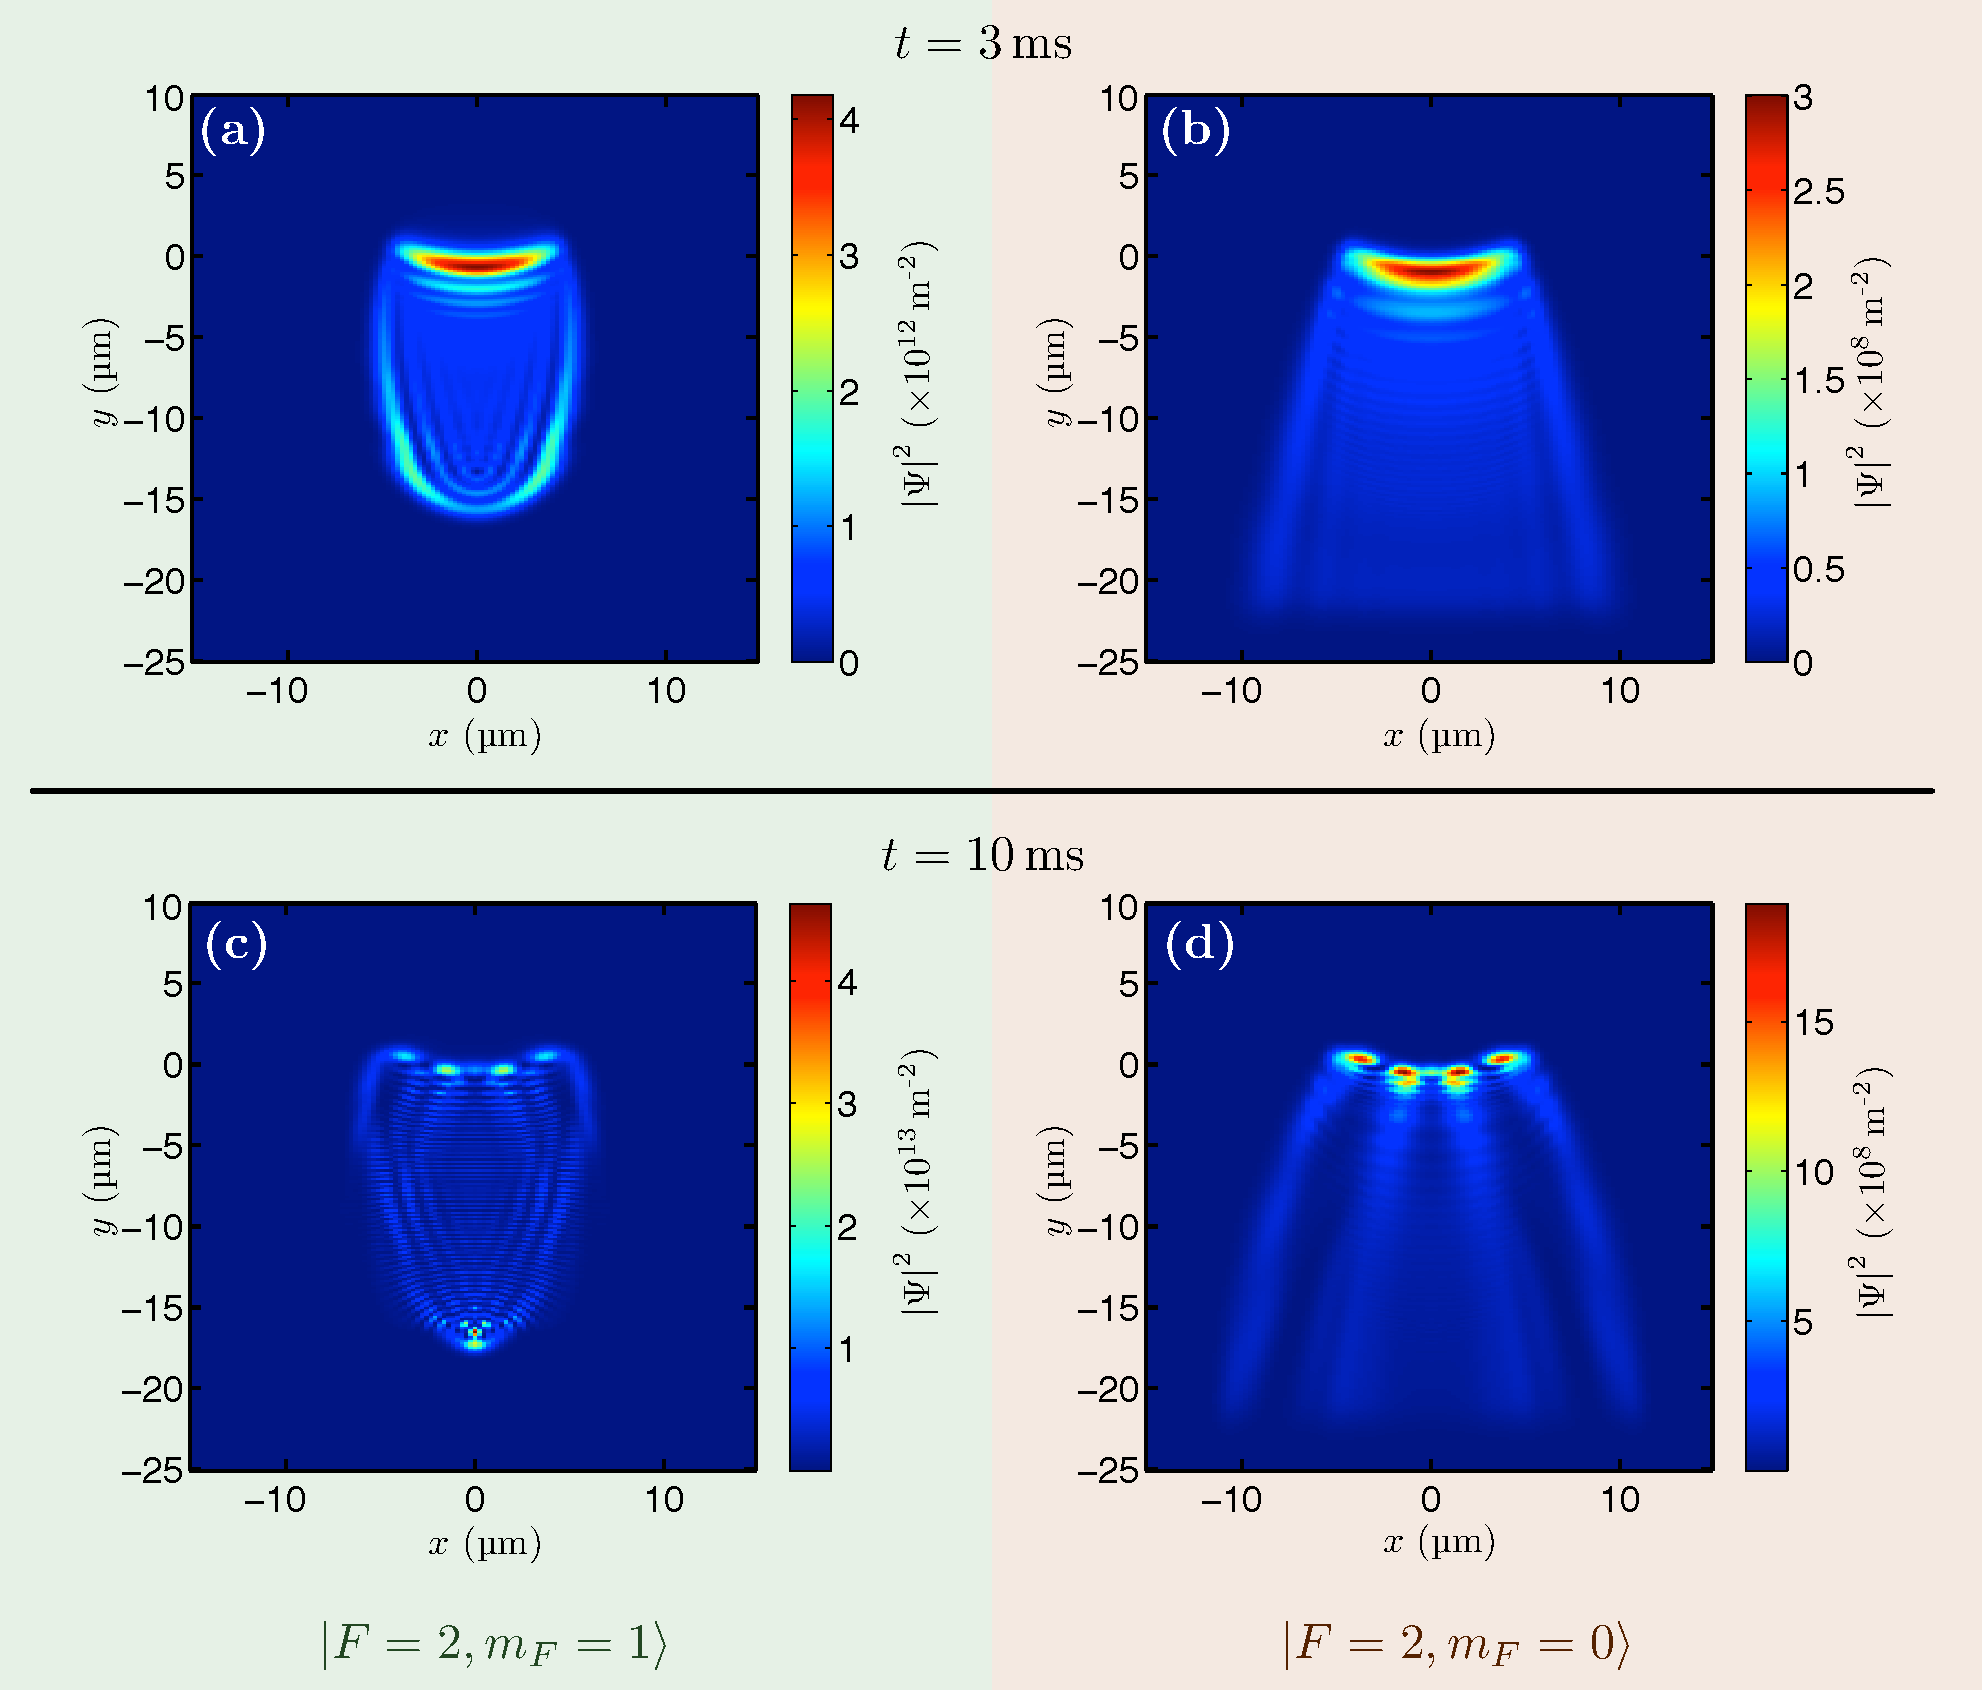
\includegraphics[width=14cm]{5LevelAtomLaserSnapshots}
    \caption{FIXME: This is not a caption. Top row: $t = \unit[3]{ms}$, bottom row: $t = \unit[10]{ms}$.  Left column is $\ket{F=2, m_F=1}$, right column is $\ket{F=2, m_F=0}$.  Note the use of absorbing boundary layers in the right column}
    \label{OpticalPumping:5LevelAtomLaserSnapshots}
\end{figure}

The difference between the spatial structures described by one- and two-dimensional models of 5-level atom laser outcoupling would have a significant affect on a pumping model.  The density spike in the $\ket{F=2, m_F=1}$ state near the classical turning point would result in a significant reduction in the pumping light intensity and a corresponding loss of atoms from the $\ket{F=2, m_F=1}$ state negatively impacting achievable pumping efficiencies.  In a one-dimensional model it will have been assumed that all of the incident pumping light over the characteristic length scale in that dimension of $x = \unit[5.9]{\micro m}$ will interact with the density spike, leading to higher losses than in a two-dimensional model in which the density spike will have its correct size of $\sim\unit[1]{\micro m}$.  It is for these reasons that a model of the continuous pumping experiment including all 5 levels of the $F=2$ manifold must be solved in at least two dimensions given that the experiment operates on the timescale of many oscillation periods in the tight trapping dimensions.  It may be necessary to solve the full three-dimensional system as the duration of the pumping experiment ($\unit[100]{ms}$--$\unit[200]{ms}$) is longer than a single oscillation period in the weak trapping dimension, $\unit[76]{ms}$.

It would be computationally intensive, although achievable, to solve a two- or three-dimensional model of the continuous pumping experiment including the full $F=2$ manifold over the pumping time of $\unit[100]{ms}$--$\unit[200]{ms}$ once or twice, it is infeasible to consider performing a parameter scan similar to that in \sectionref{OpticalPumping:3LevelModel} in which hundreds or thousands of runs of the simulation would be necessary.  Although such a system cannot yet be investigated numerically, the problems posed by the 5-level nature of the atom laser outcoupling is not fundamental to the pumping process itself.  These are technical issues that relate to the transport of atoms to the lasing condensate, not fundamental issues affecting the pumping process itself.


\subsection{The pulsed pumping experiment}
\label{OpticalPumping:PulsedPumpingExperiment}

This section describes the pulsed pumping experiment \citep{Doring:2009}, its motivations and results.  We also discuss the theoretical results and comparison to experiment.  Basically just steal figures from the paper.  The experiment focussed on the $2 \hbar k$ momentum-transfer process, and a discussion is needed as to why this process doesn't directly correspond to the $2 \hbar k$ momentum-transfer process in the continuous experiment.  The conclusions of this section are that although there is reasonable agreement in the operation of the pumping process, there is anomalously low heating observed in the experiment.  This suggests that there is beyond mean-field physics occurring here suppressing spontaneous emission.  The likely candidate is BAR.

\parasep

The pulsed pumping experiment had the same basic set up as the continuous experiment, but instead a pulse of atoms (the \emph{transfer pulse}) was outcoupled from the upper condensate.  As this pulse was outcoupled over $\unit[100]{\micro s}$ (or whatever time it was) the issue of detuning essentially doesn't arise.  The Fourier width of the outcoupling pulse is large enough to essentially outcouple a copy of the condensate into the different Zeeman levels.  This transfer pulse was allowed to fall a variable delay time before pulsing on the same pumping light used in the continuous experiment.  The transfer pulse was finally allowed to fall further before imaging to determine the number of atoms remaining in the transfer pulse.  Due to the vastly different densities of the condensate and the transfer pulse, it is impossible to simultaneously measure the size of each.  Moreover, as the transfer pulse is significantly smaller than the target condensate, it was impossible to determine the number of transferred atoms to the target condensate.

\subsubsection{Theory / Experiment comparison}

We have good agreement with the loss of atoms out of the transfer pulse, which suggests that the $2 \hbar k$ resonance is workable, although it must be realised that operating a pulsed experiment is fundamentally different to the operation of the continuous experiment.  One model for the operation of the continuous experiment suggests that a process like STIRAP is occurring in the spatial domain instead of the usual temporal domain.  By operating the experiment in the pulsed regime, we are able to cause this process to occur in the temporal domain again, allowing access to the $2 \hbar k$ resonance.  Regardless, there are some questions that remain unanswered.  While we have good agreement on the transfer of atoms \emph{out} of the pulse, the experiment has no information about the transfer of atoms \emph{into} the condensate.  For this question, we can only rely on the theory.  In this case, the theory suggests that there should be a significant number of photons emitted spontaneously within the lower condensate.  A single one of these photons should cause significant (observable) heating of the lower condensate.  The issue is that no such heating is observed.  We are left scratching our heads on this issue (see next section).

\section{Discussion / Outlook}
\label{OpticalPumping:Discussion}

This is where we say that we have reasonable evidence to say that we know what is going on in the transfer of atoms to the lower condensate, but a pretty poor explanation for what happens afterwards.  It is precisely this latter process that was thought to prevent optical pumping of condensates, and so the fact that the expected heating has not been observed is of great interest.  We can speculate wildly as to the origin of this absent heating, including BAR and quantum-mechanical collective effects due to the coherence of the atom laser.

It is hard to make any strong statements that it is the $0 \hbar k$ momentum-transfer process and not the $2 \hbar k$ momentum-transfer process given that it appears the mean-field model presented does not represent the spontaneous losses accurately.  However, the dark-state following argument doesn't really rely on spontaneous losses.  So, we have strong indications that it is the $0 \hbar k$ momentum-transfer process, but we can't be sure until the anomalously low heating observed in the pulsed pumping experiment can be resolved adequately.  To resolve this, we need to theoretically model and solve the full 3D atom--light coupled system treating spontaneous emission and rescattering fully for at least a short time after the pumping light is applied (the fall of the atomic pulses can be considered normally).

\section{Conclusion}

The conclusion I have been thinking of at the moment is along the following lines.  There have been three parts to the optical pumping process: (i) the delivery of atoms in an appropriate state to the condensate being pumped; (ii) the transfer of those atoms to the condensate being pumped; and (iii) the behaviour of the emitted photons within the pumped condensate.  This present chapter has aimed to understand part (ii) of this process.  Ideally we would also like to understand (iii) as it appears that there is some very interesting physics occurring in this part of the process, however we have fallen short of this goal.  By contrast process (i) is a technical detail of getting atoms to the lower condensate with an appropriate mode.  There are several methods that could be used for this process, and there are a number of arguments why the models used in this chapter are unsuitable for fully describing process (i).  Technical details are of course important, but not of fundamental importance.  And it has been the fundamentally important processes that we have aimed to investigate in the present chapter.
